% Generated by Sphinx.
\def\sphinxdocclass{report}
\documentclass[letterpaper,10pt,english]{sphinxmanual}
\usepackage[utf8]{inputenc}
\DeclareUnicodeCharacter{00A0}{\nobreakspace}
\usepackage{cmap}
\usepackage[T1]{fontenc}
\usepackage{babel}
\usepackage{times}
\usepackage[Bjarne]{fncychap}
\usepackage{longtable}
\usepackage{sphinx}
\usepackage{multirow}
\usepackage{amsfonts}

\title{Econ 133 Lecture Notes}
\date{March 11, 2014}
\release{Security Markets and Financial Institutions}
\author{Eric M. Aldrich}
\newcommand{\sphinxlogo}{}
\renewcommand{\releasename}{}
\makeindex

\makeatletter
\def\PYG@reset{\let\PYG@it=\relax \let\PYG@bf=\relax%
    \let\PYG@ul=\relax \let\PYG@tc=\relax%
    \let\PYG@bc=\relax \let\PYG@ff=\relax}
\def\PYG@tok#1{\csname PYG@tok@#1\endcsname}
\def\PYG@toks#1+{\ifx\relax#1\empty\else%
    \PYG@tok{#1}\expandafter\PYG@toks\fi}
\def\PYG@do#1{\PYG@bc{\PYG@tc{\PYG@ul{%
    \PYG@it{\PYG@bf{\PYG@ff{#1}}}}}}}
\def\PYG#1#2{\PYG@reset\PYG@toks#1+\relax+\PYG@do{#2}}

\expandafter\def\csname PYG@tok@gd\endcsname{\def\PYG@tc##1{\textcolor[rgb]{0.63,0.00,0.00}{##1}}}
\expandafter\def\csname PYG@tok@gu\endcsname{\let\PYG@bf=\textbf\def\PYG@tc##1{\textcolor[rgb]{0.50,0.00,0.50}{##1}}}
\expandafter\def\csname PYG@tok@gt\endcsname{\def\PYG@tc##1{\textcolor[rgb]{0.00,0.27,0.87}{##1}}}
\expandafter\def\csname PYG@tok@gs\endcsname{\let\PYG@bf=\textbf}
\expandafter\def\csname PYG@tok@gr\endcsname{\def\PYG@tc##1{\textcolor[rgb]{1.00,0.00,0.00}{##1}}}
\expandafter\def\csname PYG@tok@cm\endcsname{\let\PYG@it=\textit\def\PYG@tc##1{\textcolor[rgb]{0.25,0.50,0.56}{##1}}}
\expandafter\def\csname PYG@tok@vg\endcsname{\def\PYG@tc##1{\textcolor[rgb]{0.73,0.38,0.84}{##1}}}
\expandafter\def\csname PYG@tok@m\endcsname{\def\PYG@tc##1{\textcolor[rgb]{0.13,0.50,0.31}{##1}}}
\expandafter\def\csname PYG@tok@mh\endcsname{\def\PYG@tc##1{\textcolor[rgb]{0.13,0.50,0.31}{##1}}}
\expandafter\def\csname PYG@tok@cs\endcsname{\def\PYG@tc##1{\textcolor[rgb]{0.25,0.50,0.56}{##1}}\def\PYG@bc##1{\setlength{\fboxsep}{0pt}\colorbox[rgb]{1.00,0.94,0.94}{\strut ##1}}}
\expandafter\def\csname PYG@tok@ge\endcsname{\let\PYG@it=\textit}
\expandafter\def\csname PYG@tok@vc\endcsname{\def\PYG@tc##1{\textcolor[rgb]{0.73,0.38,0.84}{##1}}}
\expandafter\def\csname PYG@tok@il\endcsname{\def\PYG@tc##1{\textcolor[rgb]{0.13,0.50,0.31}{##1}}}
\expandafter\def\csname PYG@tok@go\endcsname{\def\PYG@tc##1{\textcolor[rgb]{0.20,0.20,0.20}{##1}}}
\expandafter\def\csname PYG@tok@cp\endcsname{\def\PYG@tc##1{\textcolor[rgb]{0.00,0.44,0.13}{##1}}}
\expandafter\def\csname PYG@tok@gi\endcsname{\def\PYG@tc##1{\textcolor[rgb]{0.00,0.63,0.00}{##1}}}
\expandafter\def\csname PYG@tok@gh\endcsname{\let\PYG@bf=\textbf\def\PYG@tc##1{\textcolor[rgb]{0.00,0.00,0.50}{##1}}}
\expandafter\def\csname PYG@tok@ni\endcsname{\let\PYG@bf=\textbf\def\PYG@tc##1{\textcolor[rgb]{0.84,0.33,0.22}{##1}}}
\expandafter\def\csname PYG@tok@nl\endcsname{\let\PYG@bf=\textbf\def\PYG@tc##1{\textcolor[rgb]{0.00,0.13,0.44}{##1}}}
\expandafter\def\csname PYG@tok@nn\endcsname{\let\PYG@bf=\textbf\def\PYG@tc##1{\textcolor[rgb]{0.05,0.52,0.71}{##1}}}
\expandafter\def\csname PYG@tok@no\endcsname{\def\PYG@tc##1{\textcolor[rgb]{0.38,0.68,0.84}{##1}}}
\expandafter\def\csname PYG@tok@na\endcsname{\def\PYG@tc##1{\textcolor[rgb]{0.25,0.44,0.63}{##1}}}
\expandafter\def\csname PYG@tok@nb\endcsname{\def\PYG@tc##1{\textcolor[rgb]{0.00,0.44,0.13}{##1}}}
\expandafter\def\csname PYG@tok@nc\endcsname{\let\PYG@bf=\textbf\def\PYG@tc##1{\textcolor[rgb]{0.05,0.52,0.71}{##1}}}
\expandafter\def\csname PYG@tok@nd\endcsname{\let\PYG@bf=\textbf\def\PYG@tc##1{\textcolor[rgb]{0.33,0.33,0.33}{##1}}}
\expandafter\def\csname PYG@tok@ne\endcsname{\def\PYG@tc##1{\textcolor[rgb]{0.00,0.44,0.13}{##1}}}
\expandafter\def\csname PYG@tok@nf\endcsname{\def\PYG@tc##1{\textcolor[rgb]{0.02,0.16,0.49}{##1}}}
\expandafter\def\csname PYG@tok@si\endcsname{\let\PYG@it=\textit\def\PYG@tc##1{\textcolor[rgb]{0.44,0.63,0.82}{##1}}}
\expandafter\def\csname PYG@tok@s2\endcsname{\def\PYG@tc##1{\textcolor[rgb]{0.25,0.44,0.63}{##1}}}
\expandafter\def\csname PYG@tok@vi\endcsname{\def\PYG@tc##1{\textcolor[rgb]{0.73,0.38,0.84}{##1}}}
\expandafter\def\csname PYG@tok@nt\endcsname{\let\PYG@bf=\textbf\def\PYG@tc##1{\textcolor[rgb]{0.02,0.16,0.45}{##1}}}
\expandafter\def\csname PYG@tok@nv\endcsname{\def\PYG@tc##1{\textcolor[rgb]{0.73,0.38,0.84}{##1}}}
\expandafter\def\csname PYG@tok@s1\endcsname{\def\PYG@tc##1{\textcolor[rgb]{0.25,0.44,0.63}{##1}}}
\expandafter\def\csname PYG@tok@gp\endcsname{\let\PYG@bf=\textbf\def\PYG@tc##1{\textcolor[rgb]{0.78,0.36,0.04}{##1}}}
\expandafter\def\csname PYG@tok@sh\endcsname{\def\PYG@tc##1{\textcolor[rgb]{0.25,0.44,0.63}{##1}}}
\expandafter\def\csname PYG@tok@ow\endcsname{\let\PYG@bf=\textbf\def\PYG@tc##1{\textcolor[rgb]{0.00,0.44,0.13}{##1}}}
\expandafter\def\csname PYG@tok@sx\endcsname{\def\PYG@tc##1{\textcolor[rgb]{0.78,0.36,0.04}{##1}}}
\expandafter\def\csname PYG@tok@bp\endcsname{\def\PYG@tc##1{\textcolor[rgb]{0.00,0.44,0.13}{##1}}}
\expandafter\def\csname PYG@tok@c1\endcsname{\let\PYG@it=\textit\def\PYG@tc##1{\textcolor[rgb]{0.25,0.50,0.56}{##1}}}
\expandafter\def\csname PYG@tok@kc\endcsname{\let\PYG@bf=\textbf\def\PYG@tc##1{\textcolor[rgb]{0.00,0.44,0.13}{##1}}}
\expandafter\def\csname PYG@tok@c\endcsname{\let\PYG@it=\textit\def\PYG@tc##1{\textcolor[rgb]{0.25,0.50,0.56}{##1}}}
\expandafter\def\csname PYG@tok@mf\endcsname{\def\PYG@tc##1{\textcolor[rgb]{0.13,0.50,0.31}{##1}}}
\expandafter\def\csname PYG@tok@err\endcsname{\def\PYG@bc##1{\setlength{\fboxsep}{0pt}\fcolorbox[rgb]{1.00,0.00,0.00}{1,1,1}{\strut ##1}}}
\expandafter\def\csname PYG@tok@kd\endcsname{\let\PYG@bf=\textbf\def\PYG@tc##1{\textcolor[rgb]{0.00,0.44,0.13}{##1}}}
\expandafter\def\csname PYG@tok@ss\endcsname{\def\PYG@tc##1{\textcolor[rgb]{0.32,0.47,0.09}{##1}}}
\expandafter\def\csname PYG@tok@sr\endcsname{\def\PYG@tc##1{\textcolor[rgb]{0.14,0.33,0.53}{##1}}}
\expandafter\def\csname PYG@tok@mo\endcsname{\def\PYG@tc##1{\textcolor[rgb]{0.13,0.50,0.31}{##1}}}
\expandafter\def\csname PYG@tok@mi\endcsname{\def\PYG@tc##1{\textcolor[rgb]{0.13,0.50,0.31}{##1}}}
\expandafter\def\csname PYG@tok@kn\endcsname{\let\PYG@bf=\textbf\def\PYG@tc##1{\textcolor[rgb]{0.00,0.44,0.13}{##1}}}
\expandafter\def\csname PYG@tok@o\endcsname{\def\PYG@tc##1{\textcolor[rgb]{0.40,0.40,0.40}{##1}}}
\expandafter\def\csname PYG@tok@kr\endcsname{\let\PYG@bf=\textbf\def\PYG@tc##1{\textcolor[rgb]{0.00,0.44,0.13}{##1}}}
\expandafter\def\csname PYG@tok@s\endcsname{\def\PYG@tc##1{\textcolor[rgb]{0.25,0.44,0.63}{##1}}}
\expandafter\def\csname PYG@tok@kp\endcsname{\def\PYG@tc##1{\textcolor[rgb]{0.00,0.44,0.13}{##1}}}
\expandafter\def\csname PYG@tok@w\endcsname{\def\PYG@tc##1{\textcolor[rgb]{0.73,0.73,0.73}{##1}}}
\expandafter\def\csname PYG@tok@kt\endcsname{\def\PYG@tc##1{\textcolor[rgb]{0.56,0.13,0.00}{##1}}}
\expandafter\def\csname PYG@tok@sc\endcsname{\def\PYG@tc##1{\textcolor[rgb]{0.25,0.44,0.63}{##1}}}
\expandafter\def\csname PYG@tok@sb\endcsname{\def\PYG@tc##1{\textcolor[rgb]{0.25,0.44,0.63}{##1}}}
\expandafter\def\csname PYG@tok@k\endcsname{\let\PYG@bf=\textbf\def\PYG@tc##1{\textcolor[rgb]{0.00,0.44,0.13}{##1}}}
\expandafter\def\csname PYG@tok@se\endcsname{\let\PYG@bf=\textbf\def\PYG@tc##1{\textcolor[rgb]{0.25,0.44,0.63}{##1}}}
\expandafter\def\csname PYG@tok@sd\endcsname{\let\PYG@it=\textit\def\PYG@tc##1{\textcolor[rgb]{0.25,0.44,0.63}{##1}}}

\def\PYGZbs{\char`\\}
\def\PYGZus{\char`\_}
\def\PYGZob{\char`\{}
\def\PYGZcb{\char`\}}
\def\PYGZca{\char`\^}
\def\PYGZam{\char`\&}
\def\PYGZlt{\char`\<}
\def\PYGZgt{\char`\>}
\def\PYGZsh{\char`\#}
\def\PYGZpc{\char`\%}
\def\PYGZdl{\char`\$}
\def\PYGZhy{\char`\-}
\def\PYGZsq{\char`\'}
\def\PYGZdq{\char`\"}
\def\PYGZti{\char`\~}
% for compatibility with earlier versions
\def\PYGZat{@}
\def\PYGZlb{[}
\def\PYGZrb{]}
\makeatother

\begin{document}

\maketitle
\tableofcontents
\phantomsection\label{index::doc}


Contents:


\chapter{Probability}
\label{probability:econ-133}\label{probability::doc}\label{probability:probability}

\section{Random Variables}
\label{probability:random-variables}
Suppose $X$ is a random variable which can take values $x
\in \mathcal{X}$.
\begin{quote}
\begin{itemize}
\item {} 
$X$ is a discrete r.v. if $\mathcal{X}$ is countable.
\begin{itemize}
\item {} 
$p(x)$ is the probability of a value $x$ and is
called the probability mass function.

\end{itemize}

\end{itemize}
\begin{itemize}
\item {} 
$X$ is a continuous r.v. if $\mathcal{X}$ is
uncountable.
\begin{itemize}
\item {} 
$f(x)$ is called the probability density function and can
be thought of as the probability of a value $x$.

\end{itemize}

\end{itemize}
\end{quote}


\section{Probability Mass Function}
\label{probability:probability-mass-function}
For a discrete random variable the \emph{probability mass function} (PMF)
is
\begin{gather}
\begin{split}p(a) = P(X = a),\end{split}\notag
\end{gather}
where $a \in \mathbb{R}$.


\section{Probability Density Function}
\label{probability:probability-density-function}
If $B = (a,b)$
\begin{gather}
\begin{split}P(X \in B) = P(a \leq X \leq b) = \int_a^b f(x) dx.\end{split}\notag
\end{gather}
Strictly speaking
\begin{gather}
\begin{split}P(X = a) = \int_a^a f(x) dx = 0,\end{split}\notag
\end{gather}
but we may (intuitively) think of $f(a) = P(X=a)$.


\section{Properties of Distributions}
\label{probability:properties-of-distributions}
For discrete random variables
\begin{quote}
\begin{itemize}
\item {} 
$p(x) \geq 0$, $\forall x \in \mathcal{X}$.

\end{itemize}
\begin{itemize}
\item {} 
$\sum_{x\in \mathcal{X}} p(x) = 1$.

\end{itemize}
\end{quote}

For continuous random variables
\begin{quote}
\begin{itemize}
\item {} 
$f(x) \geq 0$, $\forall x \in \mathcal{X}$.

\end{itemize}
\begin{itemize}
\item {} 
$\int_{x\in \mathcal{X}} f(x)dx = 1$.

\end{itemize}
\end{quote}


\section{Cumulative Distribution Function}
\label{probability:cumulative-distribution-function}
For discrete random variables the cumulative distribution function
(CDF) is
\begin{itemize}
\item {} 
$F(a) = P(X \leq a) = \sum_{x \leq a} p(x).$

\end{itemize}

For continuous random variables the CDF is
\begin{itemize}
\item {} 
$F(a) = P(X \leq a) = \int_{-\infty}^a f(x) dx.$

\end{itemize}


\section{Expected Value}
\label{probability:expected-value}
For a discrete r.v. $X$, the expected value is
\begin{gather}
\begin{split}E[X] = \sum_{x\in \mathcal{X}} x p(x).\end{split}\notag
\end{gather}
For a continuous r.v. $X$, the expected value is
\begin{gather}
\begin{split}E[X] = \int_{x\in \mathcal{X}} x \, f(x) dx.\end{split}\notag
\end{gather}

\section{Expected Value}
\label{probability:id1}
If $Y = g(X)$, then
\begin{itemize}
\item {} 
For discrete r.v. $X$

\end{itemize}
\begin{gather}
\begin{split}E[Y] = E[g(X)] = \sum_{x \in \mathcal{X}} g(x)p(x).\end{split}\notag
\end{gather}\begin{itemize}
\item {} 
For continuous r.v. $X$

\end{itemize}
\begin{gather}
\begin{split}E[Y] = E[g(X)] = \int_{x \in \mathcal{X}} g(x)f(x)dx.\end{split}\notag
\end{gather}

\section{Properties of Expectation}
\label{probability:properties-of-expectation}
For random variables $X$ and $Y$ and constants $a,b
\in \mathbb{R}$, the expected value has the following properties (for
both discrete and continuous r.v.'s):
\begin{quote}
\begin{itemize}
\item {} 
$E[aX + b] = aE[X] + b.$

\end{itemize}
\begin{itemize}
\item {} 
$E[X + Y] = E[X] + E[Y].$

\end{itemize}
\end{quote}

Realizations of $X$, denoted by $x$, may be larger or
smaller than $E[X]$.
\begin{itemize}
\item {} 
If you observed many realizations of $X$, $E[X]$ is
roughly an average of the values you would observe.

\end{itemize}


\section{Properties of Expectation - Proof}
\label{probability:properties-of-expectation-proof}\begin{gather}
\begin{split}E[aX + b] & = \int_{-\infty}^{\infty} (ax+b)f(x) dx \\
& = \int_{-\infty}^{\infty} a x f(x) dx +
\int_{-\infty}^{\infty} b f(x) dx \\
& = a \int_{-\infty}^{\infty} x f(x) dx + b
\int_{-\infty}^{\infty} f(x) dx \\
& = a\,E[X] + b.\end{split}\notag
\end{gather}

\section{Variance}
\label{probability:variance}
Generally speaking, variance is defined as
\begin{gather}
\begin{split}Var(X) = E\left[(X - E[X])^2\right].\end{split}\notag
\end{gather}
If $X$ is discrete:
\begin{gather}
\begin{split}Var(X) = \sum_{x\in \mathcal{X}} (x - E[X])^2 p(x).\end{split}\notag
\end{gather}
If $X$ is continuous:
\begin{gather}
\begin{split}Var(X) & = \int_{x\in \mathcal{X}} (x - E[X])^2 f(x) dx\end{split}\notag\\\begin{split}\end{split}\notag
\end{gather}

\section{Variance}
\label{probability:id2}
Using the properties of expectations, we can show $Var(X) =
E[X^2] - E[X]^2$:
\begin{gather}
\begin{split}Var(X) & = E\left[(X - E[X])^2\right] \\
& = E\left[X^2 - 2XE[X] + E[X]^2\right] \\
& = E[X^2] - 2E[X]E[X] + E[X]^2 \\
& = E[X^2] - E[X]^2.\end{split}\notag
\end{gather}

\section{Standard Deviation}
\label{probability:standard-deviation}
The standard deviation is simply
\begin{gather}
\begin{split}Std(X) = \sqrt{Var(X)}.\end{split}\notag
\end{gather}\begin{itemize}
\item {} 
$Std(X)$ is in the same units as $X$.

\end{itemize}
\begin{itemize}
\item {} 
$Var(X)$ is in units squared.

\end{itemize}


\section{Covariance}
\label{probability:covariance}
For two random variables $X$ and $Y$, the covariance is
generally defined as
\begin{gather}
\begin{split}Cov(X,Y)  = E\left[(X-E[X])(Y-E[Y])\right]\end{split}\notag
\end{gather}
Note that $Cov(X,X) = Var(X)$.


\section{Covariance}
\label{probability:id3}
Using the properties of expectations, we can show
\begin{gather}
\begin{split}Cov(X,Y) = E[XY] - E[X]E[Y].\end{split}\notag
\end{gather}
This can be proven in the exact way that we proved
\begin{gather}
\begin{split}Var(X) = E[X^2] - E[X]^2.\end{split}\notag
\end{gather}
In fact, note that
\begin{gather}
\begin{split}Cov(X,X) & = E[XY] - E[X]E[Y] \\
& = E[X^2] - E[X]^2 = Var(X).\end{split}\notag
\end{gather}

\section{Properties of Variance}
\label{probability:properties-of-variance}
Given random variables $X$ and $Y$ and constants
$a,b \in \mathbb{R}$,
\begin{gather}
\begin{split}Var(aX + b) = a^2Var(X).\end{split}\notag\\\begin{split}\end{split}\notag
\end{gather}\begin{gather}
\begin{split}Var(aX+bY) & = a^2Var(X) + b^2Var(Y) \\
& \hspace{3in} + 2abCov(X,Y).\end{split}\notag
\end{gather}
The latter property can be generalized to
\begin{gather}
\begin{split}Var\left(\sum_{i=1}^n a_i X_i \right) & =
\sum_{i=1}^n a_i^2Var(X_i) \\
& \hspace{1in} + 2 \sum_{i=1}^{n-1} \sum_{j=i+1}^n
a_i a_j Cov(X_i, X_j).\end{split}\notag
\end{gather}

\section{Properties of Variance - Proof}
\label{probability:properties-of-variance-proof}\begin{gather}
\begin{split}Var&(aX+bY) = E\left[(aX+bY)^2\right] - E\left[aX+bY\right]^2 \\
& = E[a^2X^2 + b^2Y^2 + 2abXY] -
\left(aE[X]+bE[Y]\right)^2 \\
& = a^2 E[X^2] + b^2 E[Y^2] + 2abE[XY] \\
& \hspace{1in} - a^2E[X]^2 - b^2E[Y]^2 -2abE[X]E[Y] \\
& = a^2 \left(E[X^2] - E[X]^2\right) + b^2
\left(E[Y^2] - E[Y]^2\right) \\
& \hspace{1.5in} + 2ab \left(E[XY] - E[X]E[Y]\right) \\
& = a^2Var(X) + b^2Var(Y) + 2abCov(X,Y).\end{split}\notag
\end{gather}

\section{Properties of Covariance}
\label{probability:properties-of-covariance}
Given random variables $W$, $X$, $Y$ and $Z$
and constants $a,b \in \mathbb{R}$,
\begin{gather}
\begin{split}Cov(X,a) = 0.\end{split}\notag\\\begin{split}\end{split}\notag
\end{gather}\begin{gather}
\begin{split}Cov(aX,bY) = abCov(X,Y).\end{split}\notag\\\begin{split}\end{split}\notag
\end{gather}\begin{gather}
\begin{split}Cov(W+X,Y+Z) & = Cov(W,Y) + Cov(W,Z) \\
& \hspace{1.3in}+ Cov(X,Y) + Cov(X,Z).\end{split}\notag
\end{gather}
The latter two can be generalized to
\begin{gather}
\begin{split}Cov\left(\sum_{i=1}^n a_i X_i, \sum_{j=1}^m b_j Y_j\right) & =
\sum_{i=1}^n \sum_{j=1}^m a_i b_j Cov(X_i, Y_j).\end{split}\notag
\end{gather}

\section{Correlation}
\label{probability:correlation}
Correlation is defined as
\begin{gather}
\begin{split}Corr(X,Y) = \frac{Cov(X,Y)}{Std(X) Std(Y)}.\end{split}\notag
\end{gather}\begin{itemize}
\item {} 
It is fairly easy to show that $-1 \leq Corr(X,Y) \leq 1$.

\end{itemize}
\begin{itemize}
\item {} 
The properties of correlations of sums of random variables follow
from those of covariance and standard deviations above.

\end{itemize}


\section{Normal Distribution}
\label{probability:normal-distribution}
The normal distribution is often used to approximate the probability
distribution of returns.
\begin{quote}
\begin{itemize}
\item {} 
It is a continuous distribution.

\end{itemize}
\begin{itemize}
\item {} 
It is symmetric.

\end{itemize}
\begin{itemize}
\item {} 
It is fully characterized by $\mu$ (mean) and $\sigma$
(standard deviation) -- i.e. if you only tell me $\mu$ and
$\sigma$, I can draw every point in the distribution.

\end{itemize}
\end{quote}


\section{Normal Density}
\label{probability:normal-density}
If $X$ is normally distributed with mean $\mu$ and
standard deviation $\sigma$, we write
\begin{gather}
\begin{split}X \sim \mathcal{N}(\mu, \sigma).\end{split}\notag
\end{gather}
The probability density function is
\begin{gather}
\begin{split}f(x) = \frac{1}{\sqrt{2\pi} \sigma}
\exp\left\{\frac{1}{2\sigma^2}(x - \mu)^2\right\}.\end{split}\notag
\end{gather}

\section{Normal Distribution}
\label{probability:id4}
From \href{http://en.wikipedia.org/wiki/Normal\_distribution}{Wikipedia}:

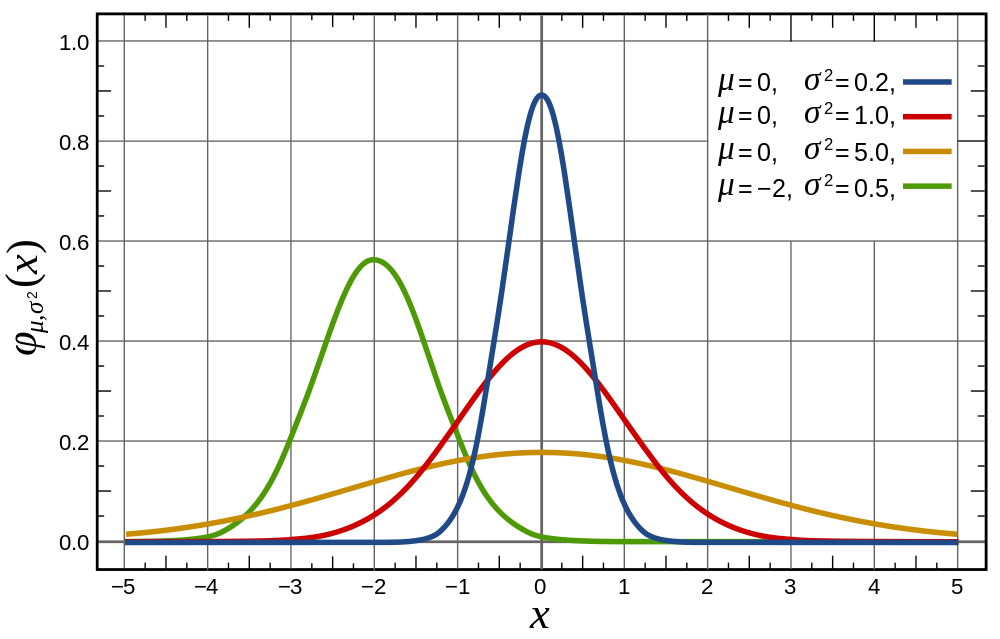
\includegraphics[width=6in]{Normal_Distribution_PDF.png}


\section{Standard Normal Distribution}
\label{probability:standard-normal-distribution}
Suppose $X \sim \mathcal{N}(\mu, \sigma)$.

Then
\begin{gather}
\begin{split}Z = \frac{X - \mu}{\sigma}\end{split}\notag\\\begin{split}\end{split}\notag
\end{gather}
is a standard normal random variable: $Z \sim
\mathcal{N}(0,1)$.
\begin{itemize}
\item {} 
That is, $Z$ has zero mean and unit standard deviation.

\end{itemize}

We can reverse the process by defining
\begin{gather}
\begin{split}X = \mu + \sigma Z.\end{split}\notag
\end{gather}

\section{Standard Normal Distribution - Proof}
\label{probability:standard-normal-distribution-proof}\begin{gather}
\begin{split}E[Z] & = E\left[\frac{X - \mu}{\sigma}\right] \\
& = \frac{1}{\sigma} E[X - \mu] \\
& = \frac{1}{\sigma} (E[X] - \mu) \\
& = \frac{1}{\sigma} (\mu - \mu) \\
& = 0.\end{split}\notag
\end{gather}

\section{Standard Normal Distribution - Proof}
\label{probability:id5}\begin{gather}
\begin{split}Var(Z) & = Var\left(\frac{X - \mu}{\sigma}\right) \\
& = Var\left(\frac{X}{\sigma} - \frac{\mu}{\sigma}\right) \\
& = \frac{1}{\sigma^2} Var(X) \\
& = \frac{\sigma^2}{\sigma^2} \\
& = 1.\end{split}\notag
\end{gather}

\section{Sum of Normals}
\label{probability:sum-of-normals}
Suppose $X_i \sim \mathcal{N}(\mu_i, \sigma_i)$ for $i =
1,\ldots,n$.

Then if we denote $W = \sum_{i=1}^n X_i$
\begin{gather}
\begin{split}W \sim \mathcal{N}\left(\sum_{i=1}^n \mu_i, \sqrt{\sum_{i=1}^n
  \sigma_i^2 + 2\sum_{i=1}^j \sum_{j=1}^n Cov(X_i, X_j)}\right).\end{split}\notag
\end{gather}
How does this simplify if $Cov(X_i, X_j) = 0$ for $i \neq
j$?


\section{Sample Mean}
\label{probability:sample-mean}
Suppose we don't know the true probabilities of a distribution, but
would like to estimate the mean.
\begin{itemize}
\item {} 
Given a sample of observations, $\{x_i\}_{i=1}^n$, of random
variable $X$, we can estimate the mean by

\end{itemize}
\begin{gather}
\begin{split}\hat{\mu} = \frac{1}{n} \sum_{i=1}^n x_i.\end{split}\notag
\end{gather}\begin{itemize}
\item {} 
This is just a simple arithmetic average, or a probability
weighted average with equal probabilities: $\frac{1}{n}$.

\end{itemize}
\begin{itemize}
\item {} 
But the true mean is a weighted average using actual (most likely,
unequal) probabilities. How do we reconcile this?

\end{itemize}


\section{Sample Mean (Cont.)}
\label{probability:sample-mean-cont}
Given that the sample $\{x_i\}_{i=1}^n$ was drawn from the
distribution of $X$, the observed values are inherently weighted by
the true probabilities (for large samples).
\begin{quote}
\begin{itemize}
\item {} 
More values in the sample will be drawn from the higher probability
regions of the distribution.

\end{itemize}
\begin{itemize}
\item {} 
So weighting all of the values equally will naturally give more
weight to the higher probability outcomes.

\end{itemize}
\end{quote}


\section{Sample Variance}
\label{probability:sample-variance}
Similarly, the sample variance can be defined as
\begin{gather}
\begin{split}\hat{\sigma}^2 & = \frac{1}{n-1} \sum_{i=1}^n (x_i - \hat{\mu})^2.\end{split}\notag
\end{gather}
Notice that we use $\frac{1}{n-1}$ instead of
$\frac{1}{n}$ for the sample average.
\begin{itemize}
\item {} 
This is because a simple average using $\frac{1}{n}$
underestimates the variability of the data because it doesn't
account for extra error involved in estimating $\hat{\mu}$.

\end{itemize}


\section{Other Sample Moments}
\label{probability:other-sample-moments}
Sample standard deviations, covariances and correlations are
computed in a similar fashion.
\begin{itemize}
\item {} 
Use the definitions above, replacing expectations with simple
averages.

\end{itemize}


\chapter{Markets}
\label{markets:markets}\label{markets::doc}
Contents:


\section{Asset Classes}
\label{assetClasses:asset-classes}\label{assetClasses::doc}

\subsection{Introduction}
\label{assetClasses:introduction}
What is an investment?
\begin{itemize}
\item {} 
A commitment of resources with the expectation of a future payoff.

\end{itemize}
\begin{itemize}
\item {} 
Financial investments: stocks, bonds, options, futures.

\end{itemize}
\begin{itemize}
\item {} 
Other investments: education, physical fitness, relationships.

\end{itemize}

Decisions faces by investors:
\begin{itemize}
\item {} 
Risk-return trade-off.

\end{itemize}
\begin{itemize}
\item {} 
Efficient pricing of financial assets.

\end{itemize}


\subsection{Real vs. Financial Assets}
\label{assetClasses:real-vs-financial-assets}
Real assets are goods (generally tangible) that are used to produce
other goods or services: buildings, machines, land, knowledge.
\begin{itemize}
\item {} 
Productivity of economy determined by real assets.

\end{itemize}

Financial assets are claims to income generated by real assets.
\begin{itemize}
\item {} 
Firms use the money raised through financial assets to invest in
plants, equipment, labor, etc.

\end{itemize}
\begin{itemize}
\item {} 
Holder of financial asset receives a portion of the resulting
returns from real assets.

\end{itemize}

While real assets determine wealth, financial assets determine
distribution of wealth.


\subsection{Equity Assets}
\label{assetClasses:equity-assets}
Equity (stock) is an ownership claim in a particular firm.
\begin{itemize}
\item {} 
Equity holder owns a prorated share of the real assets of a firm and
is entitled to a portion of the profits that is not reinvested
(dividends).

\end{itemize}
\begin{itemize}
\item {} 
The return to an equity asset is not guaranteed: it is tied to the
financial well-being of the firm.

\end{itemize}


\subsection{Equity Example}
\label{assetClasses:equity-example}
Consider \href{http://bit.ly/1ckSWAC}{The Coca-Cola Company}.
\begin{itemize}
\item {} 
On 14 Jan 2014, there were 4.42 billion shares of KO
outstanding.

\end{itemize}
\begin{itemize}
\item {} 
On 28 Nov 2013, KO decided to pay \$1.24 billion in dividends to
shareholders.

\end{itemize}
\begin{itemize}
\item {} 
This amounted to \$0.28 paid to each share.

\end{itemize}
\begin{itemize}
\item {} 
If the company were liquidated, each share would entitle the holder
to 1/4,420,000,000 of all KO assets.

\end{itemize}


\subsection{Equity Prices}
\label{assetClasses:equity-prices}
There are several ways to think about the price of an equity share.
\begin{itemize}
\item {} 
Add the values of all firm assets and divide by the number of shares
outstanding.

\end{itemize}
\begin{itemize}
\item {} 
Alternatively, it is the \href{http://en.wikipedia.org/wiki/Present\_value}{present value} of all future
payments (dividends).

\end{itemize}
\begin{gather}
\begin{split}P = \sum_{t=1}^{\infty} \frac{D_t}{(1+r)^t}\end{split}\notag
\end{gather}\begin{itemize}
\item {} 
$D_t$ represents the dividend payment at future date
$t$, and $r$ is the competitive interest rate that you could otherwise earn on your money.

\end{itemize}


\subsection{Present Value}
\label{assetClasses:id1}
Recall that present value is a way to value future payments in current
terms.
\begin{itemize}
\item {} 
Money paid to you in the future should be less than money paid now.

\end{itemize}
\begin{itemize}
\item {} 
Why?

\end{itemize}


\subsection{Present Value}
\label{assetClasses:id2}
Suppose you can earn 10\% interest on every dollar you save tonight.
\begin{itemize}
\item {} 
Then if you save \$0.9091 tonight, it will be worth
\$0.9091 $\times$ 1.1 = \$1 tomorrow.

\end{itemize}
\begin{itemize}
\item {} 
If I offer you either \$0.92 today or \$1 tomorrow, which would you
pick?

\end{itemize}
\begin{itemize}
\item {} 
If I offer you either \$0.90 today or \$1 tomorrow, which would you
pick?

\end{itemize}


\subsection{Fixed Income Assets}
\label{assetClasses:fixed-income-assets}
Fixed income securities are assets with payments determined by a
formula (e.g. bonds).
\begin{itemize}
\item {} 
U.S. Treasury bills/bonds, commercial paper, CDs.

\end{itemize}
\begin{itemize}
\item {} 
Although fixed income payments are determined
mathematically there is still risk (interest rate risk, default
risk).

\end{itemize}
\begin{itemize}
\item {} 
Longer maturity fixed income assets tend to be more risky.

\end{itemize}
\begin{itemize}
\item {} 
Fixed income is typically less risky than equity because the
payments are guaranteed.

\end{itemize}


\subsection{Fixed Income Assets}
\label{assetClasses:id3}\begin{itemize}
\item {} 
Fixed income assets are typically a way for firms or governments to
borrow money.

\end{itemize}
\begin{itemize}
\item {} 
It is possible to hold both equity and debt (fixed income) assets
for the same firm.

\end{itemize}


\subsection{Fixed Income Prices}
\label{assetClasses:fixed-income-prices}
Fixed income assets typically promise a stream of payments at future
dates.
\begin{itemize}
\item {} 
Coupon payments at regular intervals.

\end{itemize}
\begin{itemize}
\item {} 
A final principal payment (face value) at the end.

\end{itemize}
\begin{itemize}
\item {} 
The price of a fixed income asset is the present value of these
payments.

\end{itemize}
\begin{gather}
\begin{split}P = \sum_{t=1}^T \frac{C_t}{(1+r)^t} + \frac{F}{(1+r)^T}.\end{split}\notag
\end{gather}

\subsection{Derivatives}
\label{assetClasses:derivatives}
Derivatives are assets whose payoffs are determined by another
(underlying) asset.
\begin{itemize}
\item {} 
Options are assets which allow the holder the option to buy or sell
an asset at a pre-specified price at a future date.

\end{itemize}
\begin{itemize}
\item {} 
Futures are contracts to buy and sell assets (real or financial) for
a pre-specified price at a future date.

\end{itemize}
\begin{itemize}
\item {} 
These assets are called derivatives because their value derives from
the value of the underlying asset.

\end{itemize}
\begin{itemize}
\item {} 
Derivatives are commonly used for hedging (insurance) but are
sometimes used for speculation, too.

\end{itemize}


\section{Indexes and Funds}
\label{indexes:indexes-and-funds}\label{indexes::doc}

\subsection{Indexes}
\label{indexes:indexes}
Indexes are weighted averages of asset characteristics.
\begin{itemize}
\item {} 
For example, it might be a weighted average of stock prices, stock
returns, or bond yields.

\end{itemize}
\begin{itemize}
\item {} 
The two most widely cited indexes are:
\begin{itemize}
\item {} 
\href{http://en.wikipedia.org/wiki/Djia}{The Dow Jones Industrial Average (DJIA)}.

\end{itemize}
\begin{itemize}
\item {} 
\href{http://en.wikipedia.org/wiki/S\%26P\_500}{The Standard and Poor's Composite 500 (S\&P 500)}.

\end{itemize}

\end{itemize}
\begin{itemize}
\item {} 
These are reported every day in \href{http://wsj.com}{common news outlets}.

\end{itemize}


\subsection{Dow Jones}
\label{indexes:dow-jones}
The Dow Jones Industrial Average (DJIA) is the oldest U.S. index,
dating to 1896.
\begin{itemize}
\item {} 
Since 1926 it has included 30 large stocks.

\end{itemize}
\begin{itemize}
\item {} 
Originally a simple average of the prices.

\end{itemize}
\begin{itemize}
\item {} 
Percentage change in the Dow was originally the return on a
portfolio consisting of one share invested in each of the stocks
in the index.

\end{itemize}


\subsection{Dow Jones}
\label{indexes:id1}\begin{itemize}
\item {} 
The DJIA is a price-weighted average: the amount of money invested
in each asset of the portfolio is proportional to the share price.

\end{itemize}
\begin{itemize}
\item {} 
Due to splits and changes in the composition of the index, the DJIA
is no longer a simple weighted average of prices.

\end{itemize}


\subsection{Price-Weighted Indexes}
\label{indexes:price-weighted-indexes}
Consider a price-weighted index of two stocks, $X$ and $Y$
.
\begin{itemize}
\item {} 
The price of $X$ is originally \$25 and increases to \$30.

\end{itemize}
\begin{itemize}
\item {} 
The price of $Y$ is originally \$100 and decreases to \$90.

\end{itemize}

Then
\begin{itemize}
\item {} 
Initial index value = $\frac{\$25+\$100}{2} = \$62.5$.

\end{itemize}
\begin{itemize}
\item {} 
Final index value = $\frac{\$30+\$90}{2} = \$60$.

\end{itemize}
\begin{itemize}
\item {} 
Percentage change = $\frac{-\$2.5}{\$62.5} = -0.04 = -4\%$.

\end{itemize}


\subsection{Price-Weighted Indexes}
\label{indexes:id2}
Note that price-weighted indexes give higher priced stocks more
weight.
\begin{itemize}
\item {} 
The percentage change in stock $X$ is:

\end{itemize}
\begin{gather}
\begin{split}\frac{\$30 - \$25}{\$25} = 0.2 = 20\%\end{split}\notag
\end{gather}\begin{itemize}
\item {} 
The percentage change in stock $Y$ is:

\end{itemize}
\begin{gather}
\begin{split}\frac{\$90 - \$100}{\$100} = -0.1 = -10\%\end{split}\notag
\end{gather}

\subsection{Price-Weighted Indexes}
\label{indexes:id3}\begin{itemize}
\item {} 
The overall percentage change in the index is

\end{itemize}
\begin{gather}
\begin{split}\% \text{change in index} = \frac{p^0_X}{p^0_X+p^0_Y} \Delta_X +
 \frac{p^0_Y}{p^0_X+p^0_Y} \Delta_Y\end{split}\notag
\end{gather}\begin{gather}
\begin{split}= 0.2 * 0.2 + 0.8 * (-0.1) = -0.04.\end{split}\notag
\end{gather}\begin{itemize}
\item {} 
$p^0_i$ is the initial price of stock $i$.

\end{itemize}
\begin{itemize}
\item {} 
$\Delta_i$ is the percentage change in the price of stock $i$.

\end{itemize}


\subsection{Splits and Price-Weighted Averages}
\label{indexes:splits-and-price-weighted-averages}
Suppose that stock $Y$ split, causing its price to fall to \$50.
\begin{itemize}
\item {} 
This would cause a large fall in the value of the index, unless an
adjustment is made to the divisor.

\end{itemize}
\begin{itemize}
\item {} 
That is, the index value before the split is

\end{itemize}
\begin{gather}
\begin{split}\frac{\$25 + \$100}{2} = \$62.5.\end{split}\notag
\end{gather}\begin{itemize}
\item {} 
The post-split divisor, $d$, should be the value such that

\end{itemize}
\begin{gather}
\begin{split}\frac{\$25 + \$50}{d} = \$62.5.\end{split}\notag
\end{gather}

\subsection{Splits and Price-Weighted Averages}
\label{indexes:id4}\begin{itemize}
\item {} 
Hence, $d$ falls from 2 to 1.2.

\end{itemize}
\begin{itemize}
\item {} 
Notice that since the split causes the price of $Y$ to fall,
it's relative weight in the portfolio will fall.

\end{itemize}
\begin{itemize}
\item {} 
Movements in the price of $Y$ will have a smaller impact on
the index.

\end{itemize}


\subsection{Standard and Poor's Composite 500}
\label{indexes:standard-and-poor-s-composite-500}
The S\&P 500 stock index has two advantages over the Dow:
\begin{itemize}
\item {} 
It is comprised of 500 large stocks, and hence is more broadly based
and a better indicator of the market as a whole.

\end{itemize}
\begin{itemize}
\item {} 
It is a value-weighted, rather than price-weighted, index.

\end{itemize}
\begin{itemize}
\item {} 
The market value or market capitalization of a firm is simply its
total value on the market: price per share times the number of
shares outstanding.

\end{itemize}
\begin{itemize}
\item {} 
A value-weighted index weights each stock in the index according to
its market cap.

\end{itemize}


\subsection{Value-Weighted Indexes}
\label{indexes:value-weighted-indexes}
If stock $X$ currently has 20 shares trading in the market and
stock $Y$ only has 1 share, the market caps for $X$ and
$Y$ are
\begin{gather}
\begin{split}MC^0_X & = 20 * \$25 = \$500\end{split}\notag
\end{gather}\begin{gather}
\begin{split}MC^0_Y & = 1*\$100=\$100.\end{split}\notag
\end{gather}\begin{itemize}
\item {} 
A value-weighted index of the two stocks would give $X$ five times
the weight as $Y$.

\end{itemize}
\begin{itemize}
\item {} 
Compare to the price-weighted index which gives $Y$ four times
the weight.

\end{itemize}
\begin{itemize}
\item {} 
Initially, the total stock on the market is equal to \$500 + \$100 =
\$600.

\end{itemize}


\subsection{Value-Weighted Indexes}
\label{indexes:id5}
After the price changes, market caps become
\begin{gather}
\begin{split}MC^1_X & = 20 * \$30 = \$600\end{split}\notag
\end{gather}\begin{gather}
\begin{split}MC^1_Y & = 1*\$90=\$90.\end{split}\notag
\end{gather}\begin{itemize}
\item {} 
The total value of stock is now \$690.

\end{itemize}
\begin{itemize}
\item {} 
If the initial value of the value weighted index was \$100, after
the price changes it would be $\$100*\frac{\$690}{\$600} =
\$115$.

\end{itemize}


\subsection{Value-Weighted Indexes}
\label{indexes:id6}\begin{itemize}
\item {} 
In this case the value of the index rises since it gives a
relatively higher weight to $X$.

\end{itemize}
\begin{gather}
\begin{split}\% \text{change in index} & = \frac{MC^0_X}{MC^0_X + MC^0_Y}
\Delta_X + \frac{MC^0_Y}{MC^0_X + MC^0_Y} \Delta_Y\end{split}\notag
\end{gather}\begin{gather}
\begin{split}= \frac{5}{6} * 0.2 + \frac{1}{6} * (-0.1) = 0.15.\end{split}\notag
\end{gather}

\subsection{Equally-Weighted Indexes}
\label{indexes:equally-weighted-indexes}
One of the advantages of price-weighted and value-weighted indexes
is that they correspond to buy-and-hold portfolio strategies:
\begin{itemize}
\item {} 
A price-weighted index is equivalent to buying and holding one share
(or an equal number of shares) of each stock in the index.

\end{itemize}
\begin{itemize}
\item {} 
A value-weighted index is equivalent to buying and holding each
share of the index in proportion to its market cap.

\end{itemize}


\subsection{Equally-Weighted Indexes (Cont.)}
\label{indexes:equally-weighted-indexes-cont}
In contrast, one could form an equally-weighted index, where all
stocks receive the exact same weight.
\begin{itemize}
\item {} 
This does not correspond to a buy-and-hold strategy.

\end{itemize}
\begin{itemize}
\item {} 
Consider starting with with equal amounts of money invested in
stocks $X$ and $Y$.

\end{itemize}
\begin{itemize}
\item {} 
If the price of $X$ increases by 20\% and the price of
$Y$ falls by 10\%, the dollar amount invested in each stock is no longer equal.

\end{itemize}
\begin{itemize}
\item {} 
To keep the investment equally weighted, you would have to sell some
shares of $X$ and buy shares of $Y$.

\end{itemize}


\subsection{Other Indexes}
\label{indexes:other-indexes}
There are a wide number of published indexes:
\begin{itemize}
\item {} 
\href{http://en.wikipedia.org/wiki/Nasdaq\_Composite}{Nasdaq Composite}.

\end{itemize}
\begin{itemize}
\item {} 
\href{http://en.wikipedia.org/wiki/NYSE\_Composite}{NYSE Composite}.

\end{itemize}
\begin{itemize}
\item {} 
\href{http://en.wikipedia.org/wiki/Wilshire\_5000}{Wilshire 5000}.

\end{itemize}
\begin{itemize}
\item {} 
Sub-indexes of the S\&P 500 and others above.

\end{itemize}

To hold these as part of a portfolio one could
\begin{itemize}
\item {} 
Buy shares of a \href{http://en.wikipedia.org/wiki/Mutual\_fund}{mutual fund} that tracks the index.

\end{itemize}
\begin{itemize}
\item {} 
Buy shares of an \href{http://en.wikipedia.org/wiki/Exchange-traded\_fund}{Exchange Traded Fund (ETF)} which is a
portfolio of the shares in the index.

\end{itemize}


\section{Trading}
\label{trading:trading}\label{trading::doc}

\subsection{Exchanges}
\label{trading:exchanges}
Most financial assets today are traded on exchanges.
\begin{itemize}
\item {} 
The first stock exchange, the \href{http://lat.ms/1jqdmAQ}{Antwerp Bourse}, was established in Antwerp, Belgium in
1460.

\end{itemize}
\begin{itemize}
\item {} 
Others were established throughout Europe in the 1500s.

\end{itemize}
\begin{itemize}
\item {} 
The oldest existing stock exchange is the \href{http://en.wikipedia.org/wiki/Amsterdam\_Stock\_Exchange}{Amsterdam Stock Exchange},
which was established in 1602.

\end{itemize}
\begin{itemize}
\item {} 
The Amsterdam Stock Exchange merged with the Paris and Brussels
exchanges in 2000 to form \href{http://en.wikipedia.org/wiki/Euronext}{Euronext}.

\end{itemize}
\begin{itemize}
\item {} 
Euronext merged with the \href{http://en.wikipedia.org/wiki/New\_York\_Stock\_Exchange}{New York Stock Exchange (NYSE)} in 2007.

\end{itemize}


\subsection{Early Trading}
\label{trading:early-trading}
For centuries, trading of financial assets consisted of exchanging
physical certificates.
\begin{itemize}
\item {} 
The New York Stock Exchange was Conceived in 1792 under a buttonwood
tree on Wall Street.

\end{itemize}
\begin{itemize}
\item {} 
24 brokers signed an agreement to exclusively deal with each other.

\end{itemize}
\begin{itemize}
\item {} 
They frequently met under the tree on Wall Street to conduct
business.

\end{itemize}


\subsection{Early Trading}
\label{trading:id1}
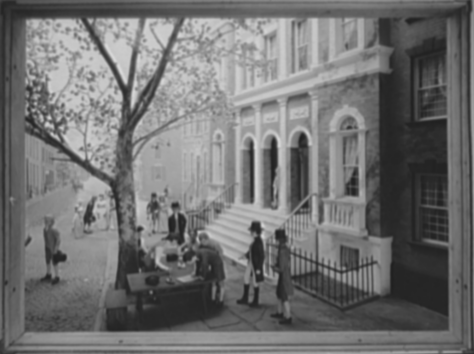
\includegraphics[width=6in]{buttonwood.png}


\subsection{Early Trading}
\label{trading:id2}\begin{quote}

{\hfill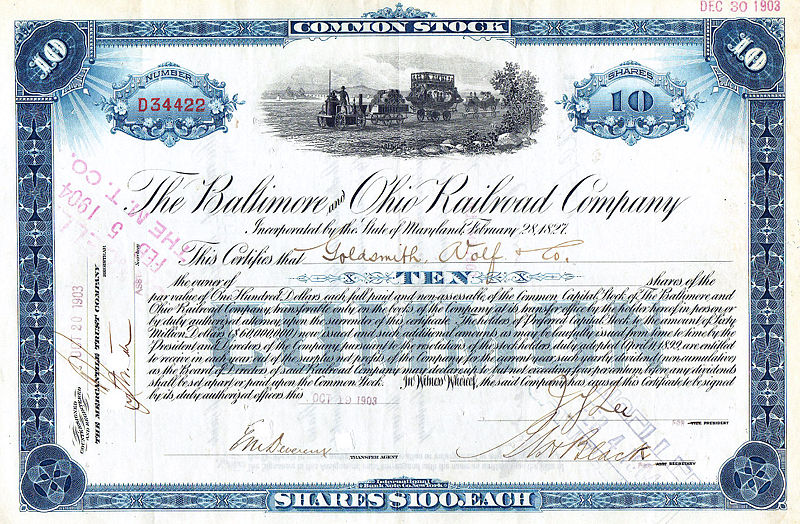
\includegraphics[width=7.5in]{stockCertificate.png}\hfill}
\end{quote}

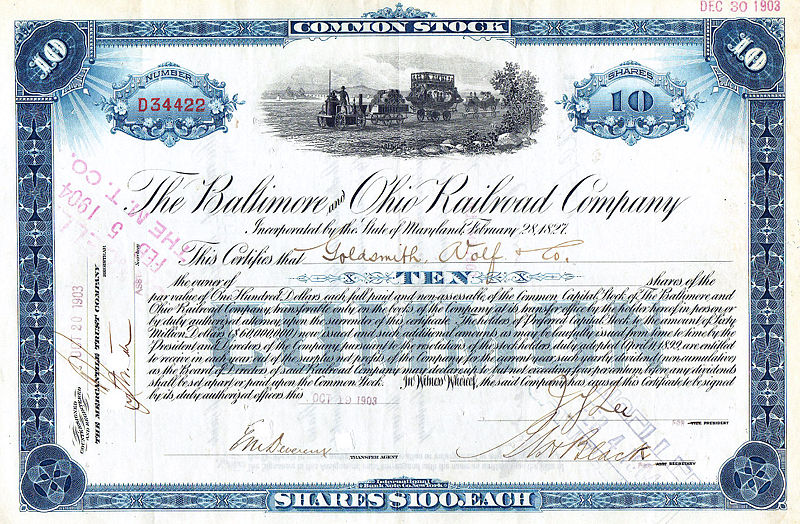
\includegraphics[width=6in]{stockCertificate.png}


\subsection{Electronic Trading}
\label{trading:electronic-trading}
In the 1990s, several electronic exchanges were developed.
\begin{itemize}
\item {} 
These are often referred to as \emph{Electronic Communication Networks}
or \href{http://www.investopedia.com/terms/e/ecn.asp}{ECNs}.

\end{itemize}
\begin{itemize}
\item {} 
\href{http://en.wikipedia.org/wiki/Island\_Exchange}{Island} was one of
the first ECNs, later purchased by \href{http://en.wikipedia.org/wiki/NASDAQ}{Nasdaq}.

\end{itemize}
\begin{itemize}
\item {} 
\href{http://en.wikipedia.org/wiki/Archipelago\_Exchange}{Archipelago}
was developed at roughly the same time and was later purchased by
NYSE (hence the name, NYSE Arca).

\end{itemize}


\subsection{High-Frequency Trading}
\label{trading:high-frequency-trading}
Originally electronic systems were simply used for quoting and
displaying prices.
\begin{itemize}
\item {} 
Trades were still executed by hand on the trading floor.

\end{itemize}
\begin{itemize}
\item {} 
Eventually, traders started placing orders electronically.

\end{itemize}
\begin{itemize}
\item {} 
This led to \emph{algorithmic trading}: traders not only submitted
orders electronically, but wrote software algorithms that
executed trades intelligently, depending on market conditions.

\end{itemize}
\begin{itemize}
\item {} 
Algorithmic trading has resulted in very fast execution, commonly
referred to as \emph{high-frequency trading}.

\end{itemize}


\subsection{Exchanges Today}
\label{trading:exchanges-today}
Exchanges today no longer consist of open floors populated by traders
yelling at each other.
\begin{itemize}
\item {} 
They consist of large warehouses, populated by computer servers
that electronically match orders.

\end{itemize}
\begin{itemize}
\item {} 
These are referred to as \emph{matching engines}.

\end{itemize}
\begin{itemize}
\item {} 
Since order execution speed is so important, many traders co-locate
their trading computers with the matching engines.

\end{itemize}


\subsection{Exchanges Today}
\label{trading:id3}\begin{itemize}
\item {} 
The NYSE Arca matching engine is located in Secaucus, NY.

\end{itemize}
\begin{itemize}
\item {} 
The \href{http://en.wikipedia.org/wiki/Chicago\_Board\_Options\_Exchange}{Chicago Board Option Exchange (CBOE)} has
co-located with NYSE Arca in Secaucus.

\end{itemize}
\begin{itemize}
\item {} 
The Nasdaq matching engine is located in Carteret, NJ.

\end{itemize}
\begin{itemize}
\item {} 
The \href{http://en.wikipedia.org/wiki/CME\_Group}{Chicago Mercantile Exchange (CME)} matching engine is
located in Aurora, IL.

\end{itemize}


\subsection{Exchanges Today}
\label{trading:id4}
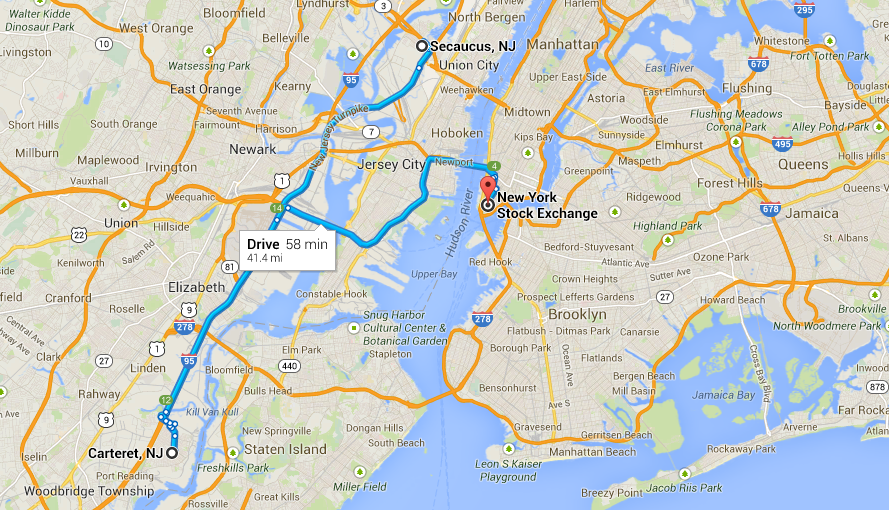
\includegraphics[width=6in]{exchangeMap.png}


\subsection{Exchanges Today}
\label{trading:id5}
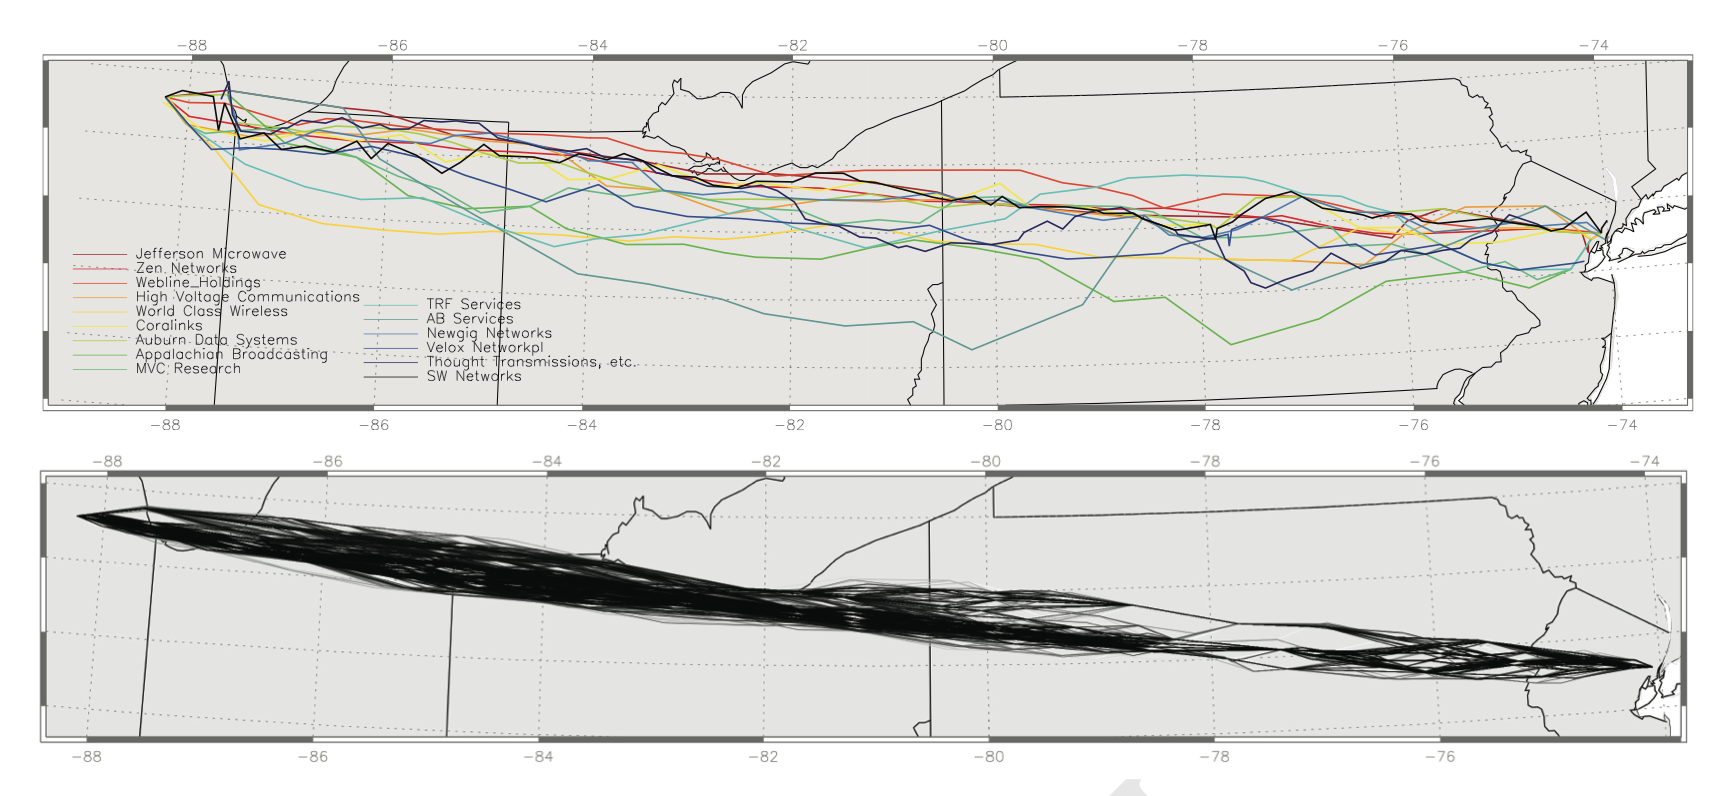
\includegraphics[width=6in]{microwave.png}


\subsection{Exchanges Today}
\label{trading:id6}
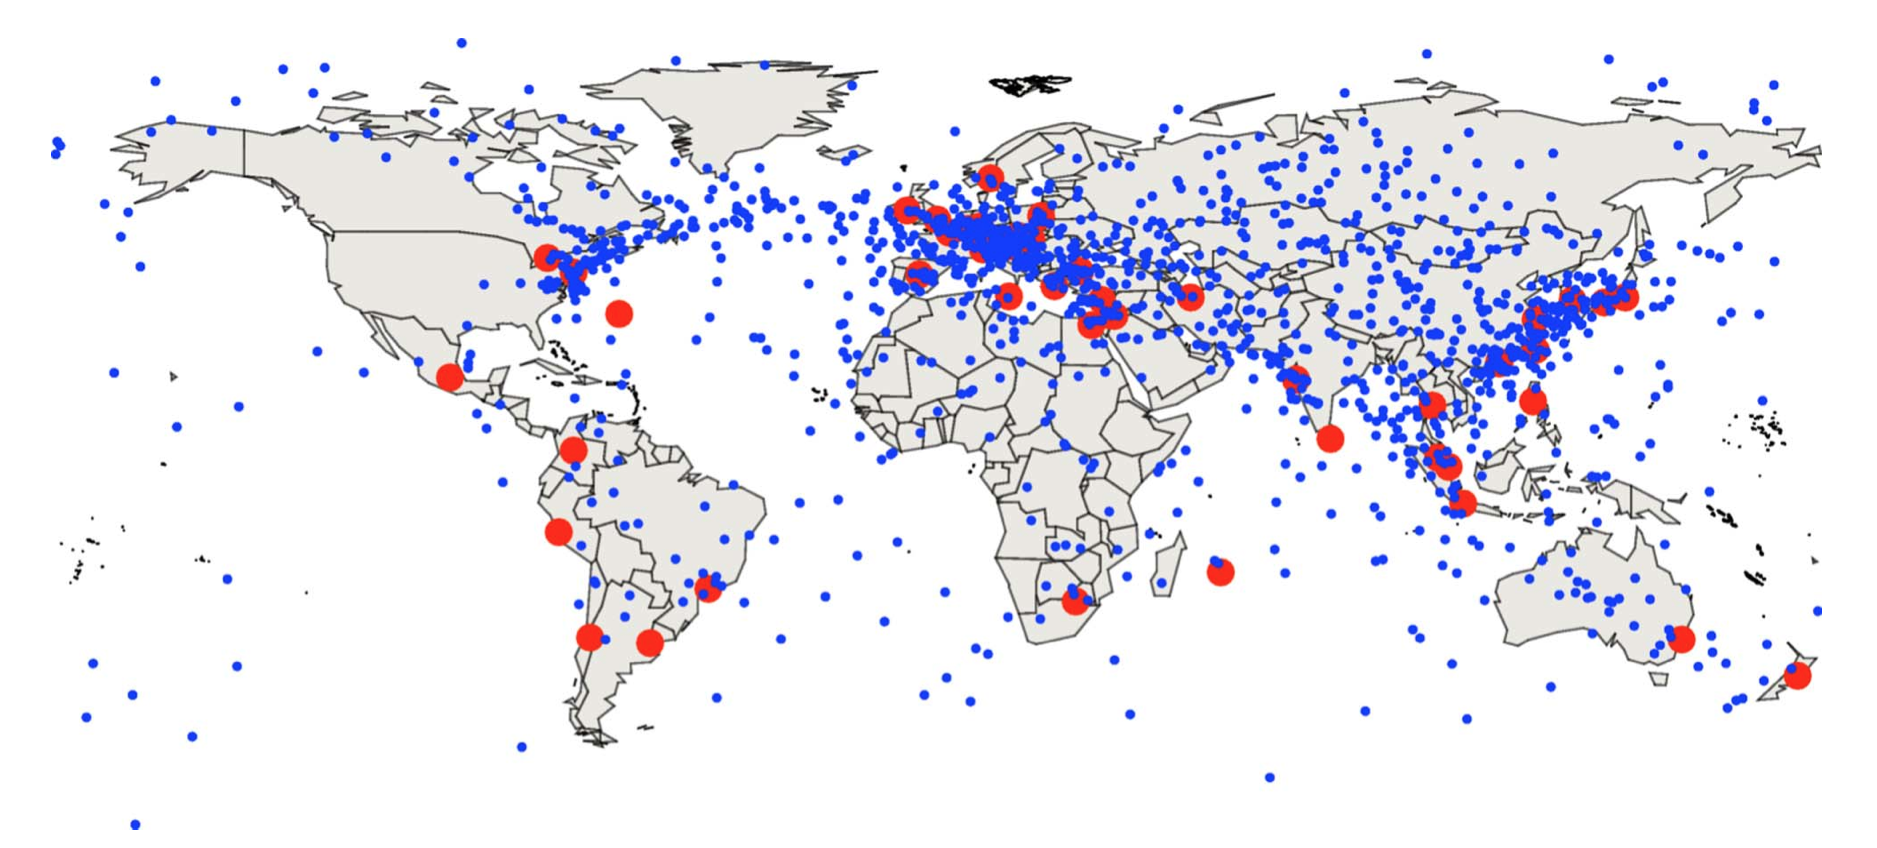
\includegraphics[width=6in]{worldExchanges.png}


\subsection{Market Makers}
\label{trading:market-makers}
Participants on exchanges include makers and takers.
\begin{itemize}
\item {} 
Makers are required to post both quotes to buy and sell assets on
the exchange.

\end{itemize}
\begin{itemize}
\item {} 
Quotes to buy are called `bids'.

\end{itemize}
\begin{itemize}
\item {} 
Quotes to sell are called `offers'.

\end{itemize}
\begin{itemize}
\item {} 
Typically there are many bids and offers posted on the exchange at
different prices.

\end{itemize}
\begin{itemize}
\item {} 
Market makers are compensated for providing quotes (also referred to
as \emph{providing liquidity}).

\end{itemize}


\subsection{Takers}
\label{trading:takers}
Takers actively \emph{take} orders that have been passively posted by
market makers.
\begin{itemize}
\item {} 
When a taker wants to buy the asset, the buy at the lowest posted
offer quote.

\end{itemize}
\begin{itemize}
\item {} 
When a take wants to sell an asset, they sell at the highest posted
bid quote.

\end{itemize}
\begin{itemize}
\item {} 
The difference between the highest bid quote and lowest offer quote
is known as the \emph{spread}.

\end{itemize}


\subsection{Order Book Example: time 1}
\label{trading:order-book-example-time-1}
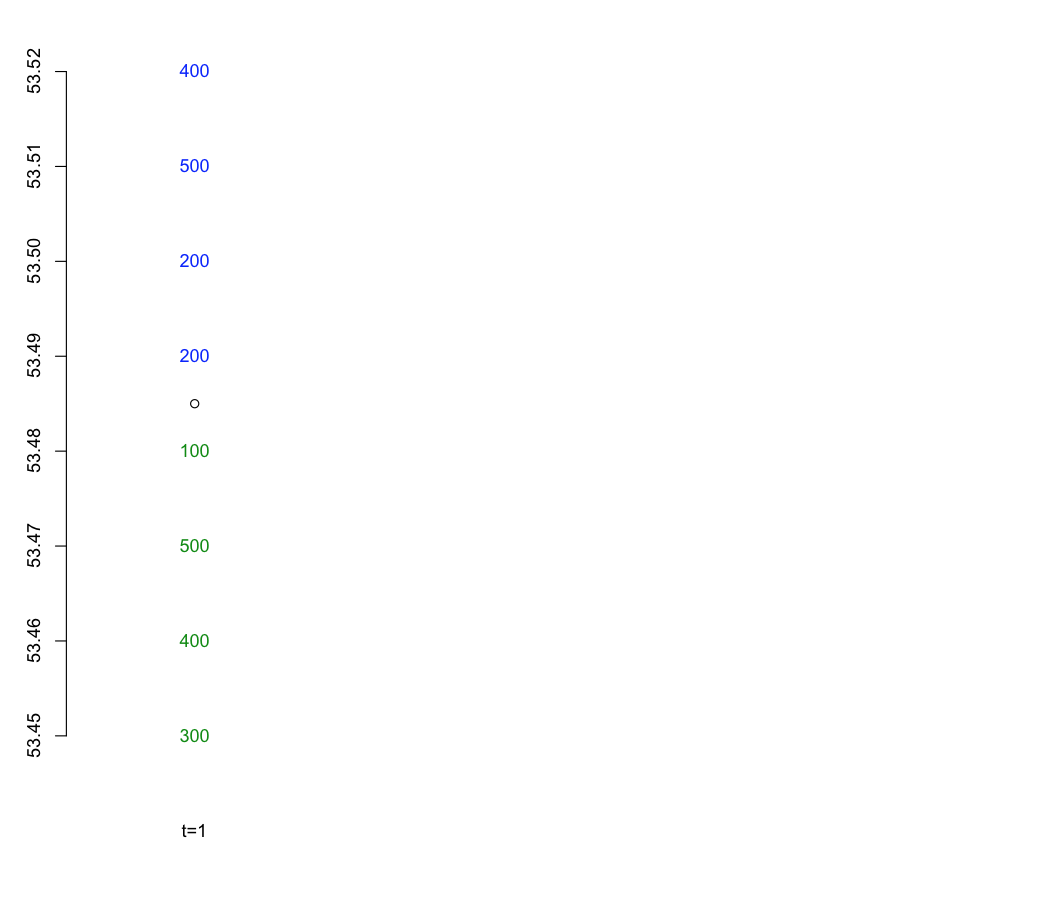
\includegraphics[width=6in]{orderBook1.png}


\subsection{Order Book Example: time 2}
\label{trading:order-book-example-time-2}
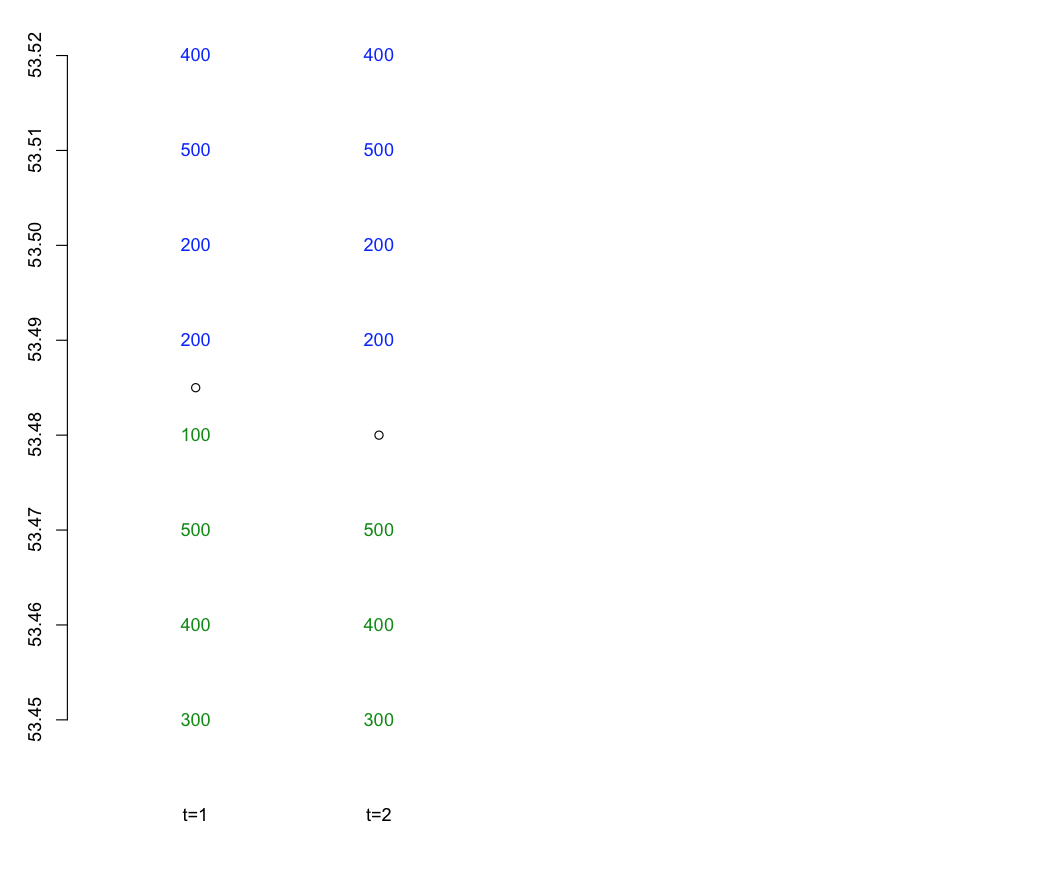
\includegraphics[width=6in]{orderBook2.png}


\subsection{Order Book Example: time 3}
\label{trading:order-book-example-time-3}
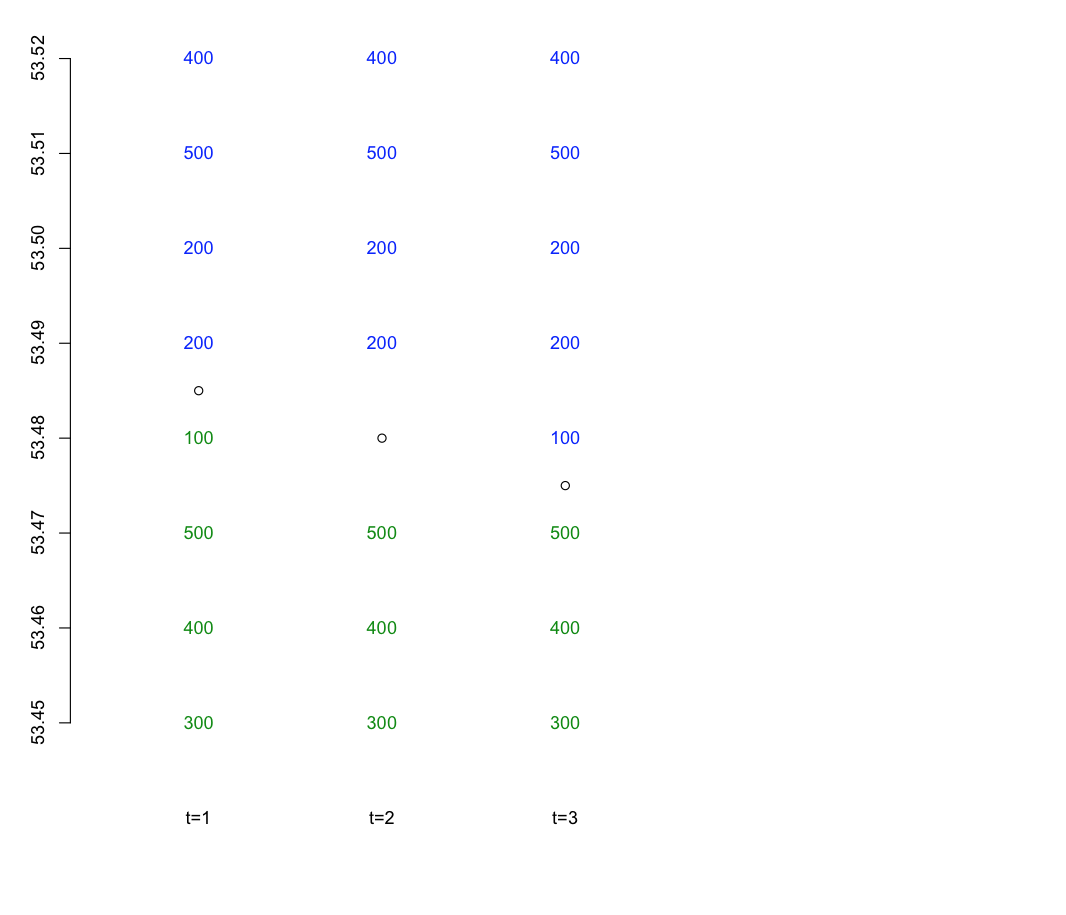
\includegraphics[width=6in]{orderBook3.png}


\subsection{Order Book Example: time 4}
\label{trading:order-book-example-time-4}
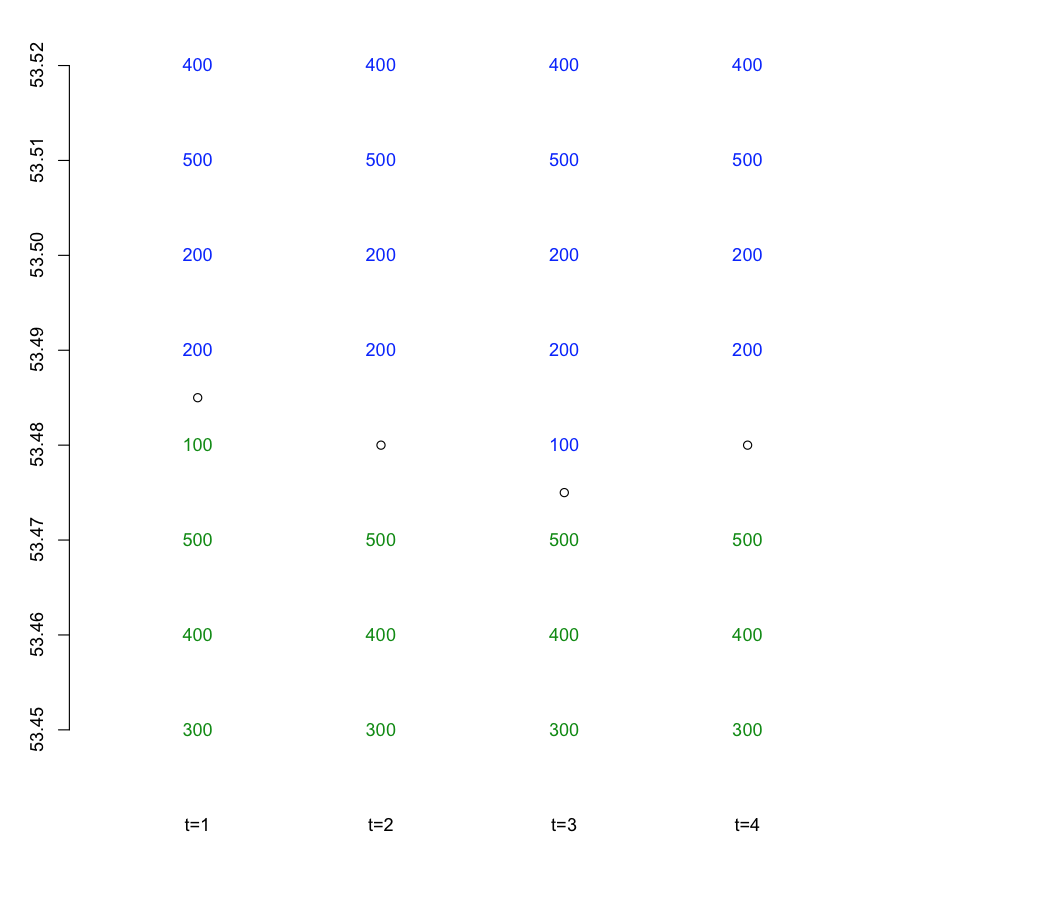
\includegraphics[width=6in]{orderBook4.png}


\subsection{Order Book Example: time 5}
\label{trading:order-book-example-time-5}
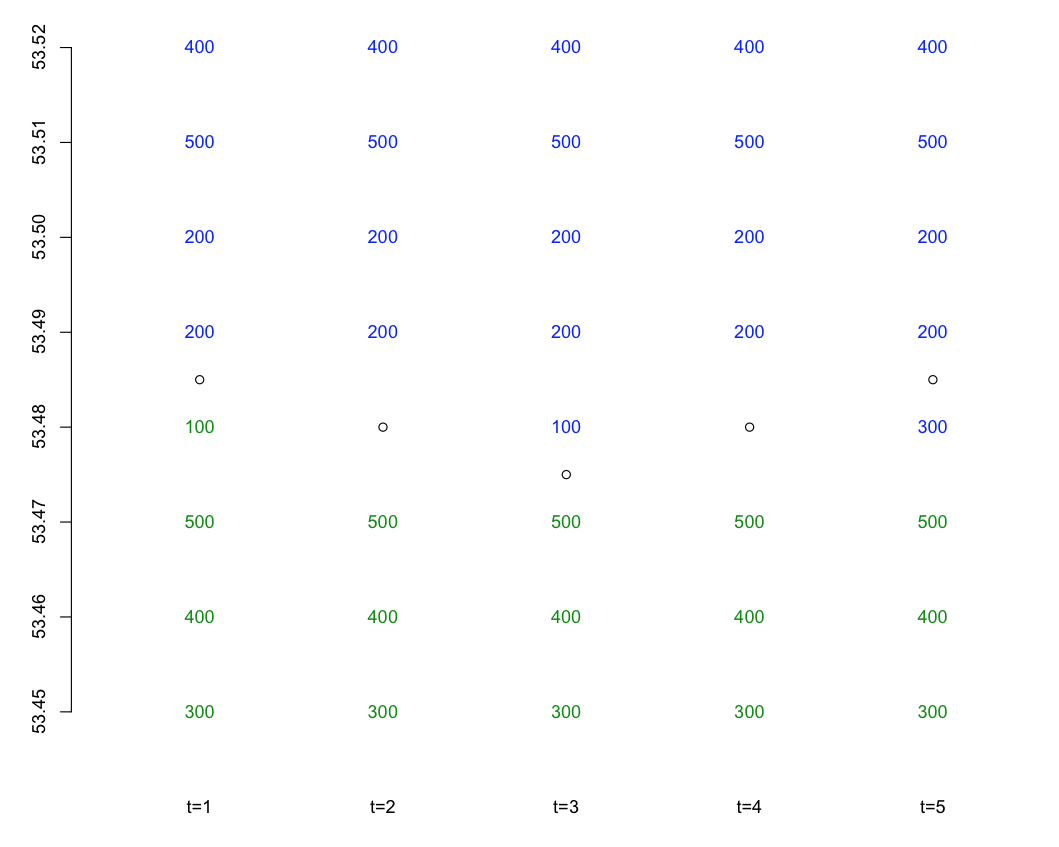
\includegraphics[width=6in]{orderBook5.png}


\subsection{Buying on Margin}
\label{trading:buying-on-margin}
When investors borrow money from a broker to purchase an asset, they
are \href{http://bit.ly/1aJfOKG}{buying on margin}.
\begin{itemize}
\item {} 
The margin is the proportion of the purchase price provided by the
investor.

\end{itemize}
\begin{itemize}
\item {} 
The purchased securities are maintained in an account by the broker
and are monitored.

\end{itemize}
\begin{itemize}
\item {} 
The Board of Governors has limited initial margins to be 50\% of the
initial purchase (i.e. investors must provide at least half of the
funds for asset purchase).

\end{itemize}


\subsection{Margin Example}
\label{trading:margin-example}
Suppose an investor has \$6000 and would like to buy 100 shares of
asset $W$, currently selling for \$100.
\begin{itemize}
\item {} 
Since \$10,000 is required for the purchase, the investor must
borrow \$4000 from a broker.

\end{itemize}
\begin{itemize}
\item {} 
The initial balance sheet would be

\end{itemize}

\begin{tabulary}{\linewidth}{|L|L|}
\hline
\textsf{\relax 
Assets
} & \textsf{\relax 
Liabilities and Owners' Equity
}\\
\hline
Value of Stock: \$10000
 & 
Loan from broker: \$4000
\\


 & 
Equity: \$6000
\\
\hline\end{tabulary}


Thus, the initial margin is $\frac{\$6000}{\$10000} = 0.6$.


\subsection{Margin Example (Cont.)}
\label{trading:margin-example-cont}
If the stock price falls to \$70 per share, the balance sheet
becomes

\begin{tabulary}{\linewidth}{|L|L|}
\hline
\textsf{\relax 
Assets
} & \textsf{\relax 
Liabilities and Owners' Equity
}\\
\hline
Value of Stock: \$7000
 & 
Loan from broker: \$4000
\\


 & 
Equity: \$3000
\\
\hline\end{tabulary}


The resulting  margin is $\frac{\$3000}{\$7000} = 0.43$.


\subsection{Maintenance Margin}
\label{trading:maintenance-margin}
Brokers can set minimal margin requirements, known as maintenance
margins.
\begin{itemize}
\item {} 
If the asset value in the account falls too low, relative to
the loan from the broker, the broker can issue a margin call.

\end{itemize}
\begin{itemize}
\item {} 
This requires the investor to add cash to the account or liquidate
some the stock.

\end{itemize}
\begin{itemize}
\item {} 
If the investor doesn't act accordingly, the broker then has
the right to sell some of the stock to pay off enough of the loan
to restore the margin to an acceptable level.

\end{itemize}


\subsection{Maintenance Margin}
\label{trading:id8}
For example, if a broker has a maintenance margin of 30\%, the
lowest the price could fall before a margin call is
\begin{gather}
\begin{split}\frac{100P - 4000}{100P} = 0.3,\end{split}\notag
\end{gather}
or P = \$57.14.


\subsection{Why Margins?}
\label{trading:why-margins}
Margins have the ability to magnify upside returns.
\begin{itemize}
\item {} 
Suppose asset $W$ is selling for \$100 and an investor
believes its price will increase to \$120 next period.

\end{itemize}
\begin{itemize}
\item {} 
If the investor buys \$10,000 worth of stock, she will realize a
return of 20\% on her money (after one period her net worth will be
\$12,000).

\end{itemize}


\subsection{Why Margins?}
\label{trading:id9}\begin{itemize}
\item {} 
However, if the investor borrows an additional \$10,000 at 5\%
interest, then she will earn a gross return of \$4000 on the
\$20,000 invested.

\end{itemize}
\begin{itemize}
\item {} 
After repaying \$10,500 (loan plus interest), her net return will be

\end{itemize}
\begin{gather}
\begin{split}\frac{(\$24, 000 - \$10, 500) - \$10, 000}{\$10,000} = 0.35.\end{split}\notag
\end{gather}\begin{itemize}
\item {} 
So the investor was able to increase her return from 20\% to 35\% by
earning a return on borrowed money.

\end{itemize}


\subsection{Why Margins?}
\label{trading:id10}
While margins provide the ability to magnify returns, they also
increase downside risk exposure.
\begin{itemize}
\item {} 
Suppose that after borrowing \$10,000 from the broker, the price of
asset $W$ fell from \$100 to \$80.

\end{itemize}
\begin{itemize}
\item {} 
The investor's gross return would be -\$4000 on the \$20,000
invested.

\end{itemize}


\subsection{Why Margins?}
\label{trading:id11}\begin{itemize}
\item {} 
After repayment of the loan, the investor's net return would be

\end{itemize}
\begin{gather}
\begin{split}\frac{(\$16,000 - \$10,500) - \$10,000}{\$10,000} = -0.45.\end{split}\notag
\end{gather}\begin{itemize}
\item {} 
If the investor hadn't borrowed money, she would have realized a net
return of -0.2. So, by borrowing on margin she has magnified her
loss from -20\% to -45\%.

\end{itemize}


\subsection{Short Sales}
\label{trading:short-sales}
\href{http://bit.ly/1bgEB8X}{Short sales} allow investors to profit from
declines in stock prices.
\begin{itemize}
\item {} 
To engage in a short sale, an investor borrows a share of a stock
from a broker and sells it on the market.

\end{itemize}
\begin{itemize}
\item {} 
The investor is then obligated to replace the share at a later date.

\end{itemize}
\begin{itemize}
\item {} 
If the stock price falls, the investor benefits from selling at a
high price and repurchasing at a low price.

\end{itemize}
\begin{itemize}
\item {} 
In between, the investor is responsible for paying the broker any
dividends that are realized (since the broker would have received
these if it hadn't lent the stock).

\end{itemize}


\subsection{Short Sales}
\label{trading:id13}\begin{itemize}
\item {} 
When an investor engages in a short sale, we say that they are
`short' the stock, or have taken the `short position'.

\end{itemize}
\begin{itemize}
\item {} 
Conversely, if an investor buys a stock (the usual transaction), we
say they are `long', or have taken the `long position'.

\end{itemize}


\subsection{Short Sale Example}
\label{trading:short-sale-example}
Suppose asset $W$ is selling for \$100 and you think its price
will fall.
\begin{itemize}
\item {} 
You decide to borrow 1000 shares, selling them for \$100 a piece,
yielding a total sale value of \$100,000.

\end{itemize}
\begin{itemize}
\item {} 
If the stock price falls to \$80 per share next period, you can
repurchase the 1000 shares for \$80,000 and return them to the
lender.

\end{itemize}
\begin{itemize}
\item {} 
You earn a total of \$20,000 in the process.

\end{itemize}


\chapter{Risk and Returns}
\label{riskReturns::doc}\label{riskReturns:risk-and-returns}
Contents:


\section{Rates of Return}
\label{returns:rates-of-return}\label{returns::doc}

\subsection{Holding Period Return}
\label{returns:holding-period-return}
Consider a stock with beginning price $P_0$, ending price
$P_1$ and a dividend payment of $d$.
\begin{itemize}
\item {} 
The \emph{holding period return} is

\end{itemize}
\begin{gather}
\begin{split}HPR & = \frac{P_1 - P_0 + d}{P_0} \\\end{split}\notag
\end{gather}\begin{gather}
\begin{split}& = \underbrace{\frac{P_1 - P_0}{P_0}}_\text{capital gains yield} +
\underbrace{\frac{d}{P_0}}_\text{dividend yield}.\end{split}\notag
\end{gather}
This definition can be used for assets other than stocks (e.g. a bond
with a coupon payment).


\subsection{Holding Period Return Example}
\label{returns:holding-period-return-example}\begin{itemize}
\item {} 
On Nov 9th 2012, Apple stock closed at $P_0 = \$547.06$.

\end{itemize}
\begin{itemize}
\item {} 
On Nov 12th, Apple payed a dividend of $d = \$2.65$ per share
and the price closed at $P_1 = \$542.83$.

\end{itemize}
\begin{itemize}
\item {} 
What was the HPR?

\end{itemize}
\begin{gather}
\begin{split}HPR & = \frac{\$542.83 - \$547.06}{\$547.06} + \frac{\$2.65}{\$547.06}\end{split}\notag
\end{gather}\begin{gather}
\begin{split}& = \frac{-\$4.23}{\$547.06} + \frac{\$2.65}{\$547.06}\end{split}\notag
\end{gather}\begin{gather}
\begin{split}& = \frac{-\$1.58}{\$547.06} = -0.00289.\end{split}\notag
\end{gather}

\subsection{Gross and Net Returns}
\label{returns:gross-and-net-returns}
Forget dividends or cash payouts for a moment.
\begin{itemize}
\item {} 
The \emph{capital gains yield} is

\end{itemize}
\begin{gather}
\begin{split}\underbrace{\frac{P_1 - P_0}{P_0}}_\text{net return}\,\,\, & =
\underbrace{\frac{P_1}{P_0}}_\text{gross return} - \,\,\,\,\, 1.\end{split}\notag
\end{gather}

\subsection{Gross and Net Returns}
\label{returns:id1}
What's the difference between net and gross returns?
\begin{itemize}
\item {} 
The net return is the fraction of your invested money that you gain
by holding the asset, excluding the original money.

\end{itemize}
\begin{itemize}
\item {} 
The gross return is the total gain, including your original
money. It is the factor by which you multiply your original invested
amount to determine the final invested amount.

\end{itemize}


\subsection{Multi-period Returns}
\label{returns:multi-period-returns}
Suppose an asset has net returns $\{r_t\}_{t=0}^{T}$. Consider two
forms of average returns:
\begin{gather}
\begin{split}\text{Arithmetic Average} & = \frac{1}{T} \sum_{t=0}^T r_t\end{split}\notag
\end{gather}
and
\begin{gather}
\begin{split}\text{Geometric Average} & = \left(\prod_{t=0}^T
(1+r_t)\right)^{\frac{1}{T}}.\end{split}\notag
\end{gather}
The geometric average is the \emph{constant} return that would
have to be earned each period to yield the same final value of the
asset.


\subsection{Annualized Returns - EAR}
\label{returns:annualized-returns-ear}
Suppose you enter into a contract to pay or receive a net rate of
return $r$ on an asset for each of $n$ periods in a year.
\begin{itemize}
\item {} 
$n=12$  is a monthly contract.

\end{itemize}
\begin{itemize}
\item {} 
$n=4$ is a quarterly contract.

\end{itemize}
\begin{itemize}
\item {} 
The Effective Annual Rate (EAR) is

\end{itemize}
\begin{gather}
\begin{split}1 + \text{EAR} & = (1 + r)^n.\end{split}\notag
\end{gather}

\subsection{Annualized Returns - APR}
\label{returns:annualized-returns-apr}
Suppose you enter into a contract to pay or receive a net rate of
return $r$ on an asset for each of $n$ periods in a year.
\begin{itemize}
\item {} 
The Annual Percentage Rate (APR) is

\end{itemize}
\begin{gather}
\begin{split}\text{APR} & = n \times r.\end{split}\notag
\end{gather}
The APR ignores compounding (as seen in the following example).


\subsection{Annualized Returns - Example}
\label{returns:annualized-returns-example}
You invest \$100 in an asset that pays 5\% return each quarter for
one year.
\begin{gather}
\begin{split}Q1: \$100 \times 1.05 = \$105\end{split}\notag
\end{gather}\begin{gather}
\begin{split}Q2: \$105 \times 1.05 = \$110.25\end{split}\notag
\end{gather}\begin{gather}
\begin{split}Q3: \$110.25 \times 1.05 = \$115.76\end{split}\notag
\end{gather}\begin{gather}
\begin{split}Q4: \$115.76 \times 1.05 = \$121.55\end{split}\notag
\end{gather}\begin{gather}
\begin{split}EAR: (1.05)^4 - 1 = 0.2155\end{split}\notag
\end{gather}\begin{gather}
\begin{split}APR: 0.05 \times 4 = 0.2\end{split}\notag
\end{gather}\begin{gather}
\begin{split}HPR: \frac{\$121.55 - \$100}{\$100} = 0.2155.\end{split}\notag
\end{gather}

\subsection{EAR and APR}
\label{returns:ear-and-apr}
What is the relationship between EAR and APR?
\begin{itemize}
\item {} 
Since

\end{itemize}
\begin{gather}
\begin{split}r = \frac{\text{APR}}{n}\end{split}\notag
\end{gather}
we have
\begin{gather}
\begin{split}1 +\text{EAR} & = \left(1 + \frac{APR}{n}\right)^n.\end{split}\notag
\end{gather}
We can rearrange the equation above to get
\begin{gather}
\begin{split}\text{APR} & = \left[(1+\text{EAR})^{\frac{1}{n}} - 1\right]
\times n.\end{split}\notag
\end{gather}

\subsection{Continuous Compounding}
\label{returns:continuous-compounding}
Continuous compounding is what occurs when we allow the number of
periods in the year, $n$, to become large.
\begin{itemize}
\item {} 
For daily returns, $n=365$.

\end{itemize}
\begin{itemize}
\item {} 
For hourly returns, $n=8760$.

\end{itemize}
\begin{itemize}
\item {} 
For returns each minute, $n=525,000$.

\end{itemize}
\begin{itemize}
\item {} 
For returns each second, $n=31,536,000$.

\end{itemize}


\subsection{Continuous Compounding}
\label{returns:id2}
Continuous compounding is the limit, when $n = \infty$. In this
case
\begin{gather}
\begin{split}\lim_{n \to \infty} \left(1 + \frac{\text{APR}}{n}\right)^n =
e^{\text{APR}}.\end{split}\notag
\end{gather}
So, under continuous compounding
\begin{gather}
\begin{split}1 + \text{EAR} & = e^{\text{APR}}\end{split}\notag
\end{gather}
or
\begin{gather}
\begin{split}\text{APR} & = \ln(1+\text{EAR}).\end{split}\notag
\end{gather}

\subsection{Inflation}
\label{returns:inflation}
Inflation is the increase of the general price level over
time.
\begin{itemize}
\item {} 
Inflation erodes the purchasing power of a given amount of
money over time.

\end{itemize}
\begin{itemize}
\item {} 
In the presence of inflation, an asset that yields a return of
$r$ doesn't actually generate $r$ units of additional real
purchasing power for each dollar invested.

\end{itemize}


\subsection{Nominal vs. Real Returns}
\label{returns:nominal-vs-real-returns}
In the previous slides we computed nominal returns.
\begin{itemize}
\item {} 
Let us momentarily change notation and refer to the nominal return
of an asset as $R$.

\end{itemize}
\begin{itemize}
\item {} 
Then the real return of the asset is the nominal return discounted
by inflation:

\end{itemize}
\begin{gather}
\begin{split}1+r & = \frac{1+R}{1+\pi}.\end{split}\notag
\end{gather}\begin{itemize}
\item {} 
$r$ is the net real return and $\pi$ is net inflation.

\end{itemize}


\subsection{Nominal vs. Real Returns}
\label{returns:id3}\begin{itemize}
\item {} 
This relationship is approximated by

\end{itemize}
\begin{gather}
\begin{split}r \approx R - \pi.\end{split}\notag
\end{gather}
See the proof on the next slide.


\subsection{Nominal vs. Real Returns - Proof}
\label{returns:nominal-vs-real-returns-proof}
The proof requires an approximation. For some small number $\epsilon >
0$,
\begin{gather}
\begin{split}\ln(1+\epsilon) & \approx \epsilon.\end{split}\notag
\end{gather}
Thus,
\begin{gather}
\begin{split}1+r & = \frac{1+R}{1+\pi}\end{split}\notag
\end{gather}\begin{gather}
\begin{split}\Rightarrow \ln(1+r) & = \ln\left(\frac{1+R}{1+\pi}\right)\end{split}\notag
\end{gather}\begin{gather}
\begin{split}\Rightarrow \ln(1+r) & = \ln(1+R) - \ln(1+\pi)\end{split}\notag
\end{gather}\begin{gather}
\begin{split}\Rightarrow r & \approx R - \pi.\end{split}\notag
\end{gather}

\subsection{Nominal vs. Real Returns - Example}
\label{returns:nominal-vs-real-returns-example}
Suppose you can invest in a CD that pays 8\% return over the next year
and that inflation is 5\% during the same period.
\begin{itemize}
\item {} 
$R = 0.08$.

\end{itemize}
\begin{itemize}
\item {} 
$\pi = 0.05$.

\end{itemize}
\begin{itemize}
\item {} 
$r \approx 0.08 - 0.05 = 0.03$.

\end{itemize}

The actual real rate of return is
\begin{gather}
\begin{split}r = \frac{1.08}{1.05} - 1 = 0.0286.\end{split}\notag
\end{gather}

\subsection{Expected Inflation}
\label{returns:expected-inflation}
In practice, future inflation is not known, even though the nominal
rate of return may be known with certainty.
\begin{itemize}
\item {} 
Think of a fixed-income asset.

\end{itemize}
\begin{itemize}
\item {} 
In this case

\end{itemize}
\begin{gather}
\begin{split}R = r + E[\pi].\end{split}\notag
\end{gather}\begin{itemize}
\item {} 
$E[\pi]$ is expected inflation.

\end{itemize}


\subsection{Expected Inflation}
\label{returns:id4}\begin{itemize}
\item {} 
The returns to typical government bonds are nominal.

\end{itemize}
\begin{itemize}
\item {} 
In 1997, the U.S. Treasury introduced ``Treasury Inflation-Protected
Securities'' (TIPS).

\end{itemize}
\begin{itemize}
\item {} 
These have coupon and principle payments that
are corrected for observed inflation over time.

\end{itemize}
\begin{itemize}
\item {} 
The difference between these rates of return on these two
instruments can be treated as a measure of expected inflation.

\end{itemize}


\section{Risk and Risk Premiums}
\label{risk:risk-and-risk-premiums}\label{risk::doc}

\subsection{Probabilistic Returns}
\label{risk:probabilistic-returns}
Since we don't know future returns, we will treat them as random
variables.
\begin{itemize}
\item {} 
We can model them as discrete random variables, taking one of a
finite set of possible values in the future: $r(s)$, $s
= 1, \ldots, S$.
\begin{itemize}
\item {} 
In this case the probability of each value is $p(s)$,
$s=1,\ldots,S$.

\end{itemize}

\end{itemize}
\begin{itemize}
\item {} 
We can model them as continuous random variables, taking one of an
infinite set of possible values in the future: $r(s)$,
$s \in \mathcal{S}$ (e.g. $\mathcal{S} = (-\infty, \infty)$).
\begin{itemize}
\item {} 
In this case the probability of each value (kind of) is
$f(s)$, $s \in \mathcal{S}$.

\end{itemize}

\end{itemize}


\subsection{Expected Returns}
\label{risk:expected-returns}
Our best guess for the future return is the expected value:
\begin{gather}
\begin{split}E[r] & \equiv \mu = \sum_{s=1}^S r(s) p(s),\end{split}\notag
\end{gather}
or
\begin{gather}
\begin{split}E[r] & \equiv \mu = \int_{s \in \mathcal{S}} r(s) f(s) dr(s).\end{split}\notag
\end{gather}

\subsection{Return Volatility}
\label{risk:return-volatility}
The amount of uncertainty in potential returns can be measured by the
variance or standard deviation.
\begin{itemize}
\item {} 
Volatility of returns specifically refers to standard deviation, NOT
VARIANCE.

\end{itemize}
\begin{gather}
\begin{split}Std(r) & \equiv \sigma = \sqrt{\sum_{s=1}^S (r(s) - \mu)^2 p(s)},\end{split}\notag
\end{gather}
or
\begin{gather}
\begin{split}Std(r) & \equiv \sigma = \sqrt{\int_{s \in \mathcal{S}} (r(s) -
\mu_r)^2 f(s) dr(s)}.\end{split}\notag
\end{gather}

\subsection{Expectation and Variance Example}
\label{risk:expectation-and-variance-example}
\begin{tabulary}{\linewidth}{|L|L|L|}
\hline
\textsf{\relax 
State
} & \textsf{\relax 
Probability
} & \textsf{\relax 
Return
}\\
\hline
Severe Recession
 & 
0.05
 & 
-0.37
\\

Mild Recession
 & 
0.25
 & 
-0.11
\\

Normal Growth
 & 
0.40
 & 
0.14
\\

Boom
 & 
0.30
 & 
0.30
\\
\hline\end{tabulary}


What are $\mu$ and $\sigma$?
\begin{gather}
\begin{split}\mu & = 0.05*(-0.37) + 0.25*(-0.11) \\
& \qquad \qquad + 0.40*0.14 + 0.30*0.30 = 0.10\end{split}\notag
\end{gather}\begin{gather}
\begin{split}E[r^2] & = 0.05*(-0.37)^2 + 0.25*(-0.11)^2 \\
& \qquad \qquad + 0.40*(0.14)^2 + 0.30*(0.30)^2 = 0.04471\end{split}\notag
\end{gather}\begin{gather}
\begin{split}\sigma & = \sqrt{E[r^2] - \mu^2} = 0.04471 - 0.10^2 = 0.03471\end{split}\notag
\end{gather}

\subsection{Assumption of Normality}
\label{risk:assumption-of-normality}
It will often be convenient to assume asset returns are normally
distributed.
\begin{itemize}
\item {} 
In this case, we will treat returns as continuous random variables.

\end{itemize}
\begin{itemize}
\item {} 
We can use the normal density function to compute probabilities of
possible events.

\end{itemize}
\begin{itemize}
\item {} 
We will not assume that returns of different assets come from the
same normal, but instead FROM DIFFERENT normal distributions.

\end{itemize}


\subsection{Differing Normal Distributions}
\label{risk:differing-normal-distributions}
As an example, suppose that
\begin{itemize}
\item {} 
Amazon stock (AMZN) has an expected monthly return of 3\% and a
volatility (standard deviation) of 8\%.

\end{itemize}
\begin{itemize}
\item {} 
Coca-Cola stock (KO) has an expected monthly return of 1\% and a
volatility (standard deviation) of 4\%.

\end{itemize}

What do their probability distributions look like?


\subsection{Amazon Distribution}
\label{risk:amazon-distribution}
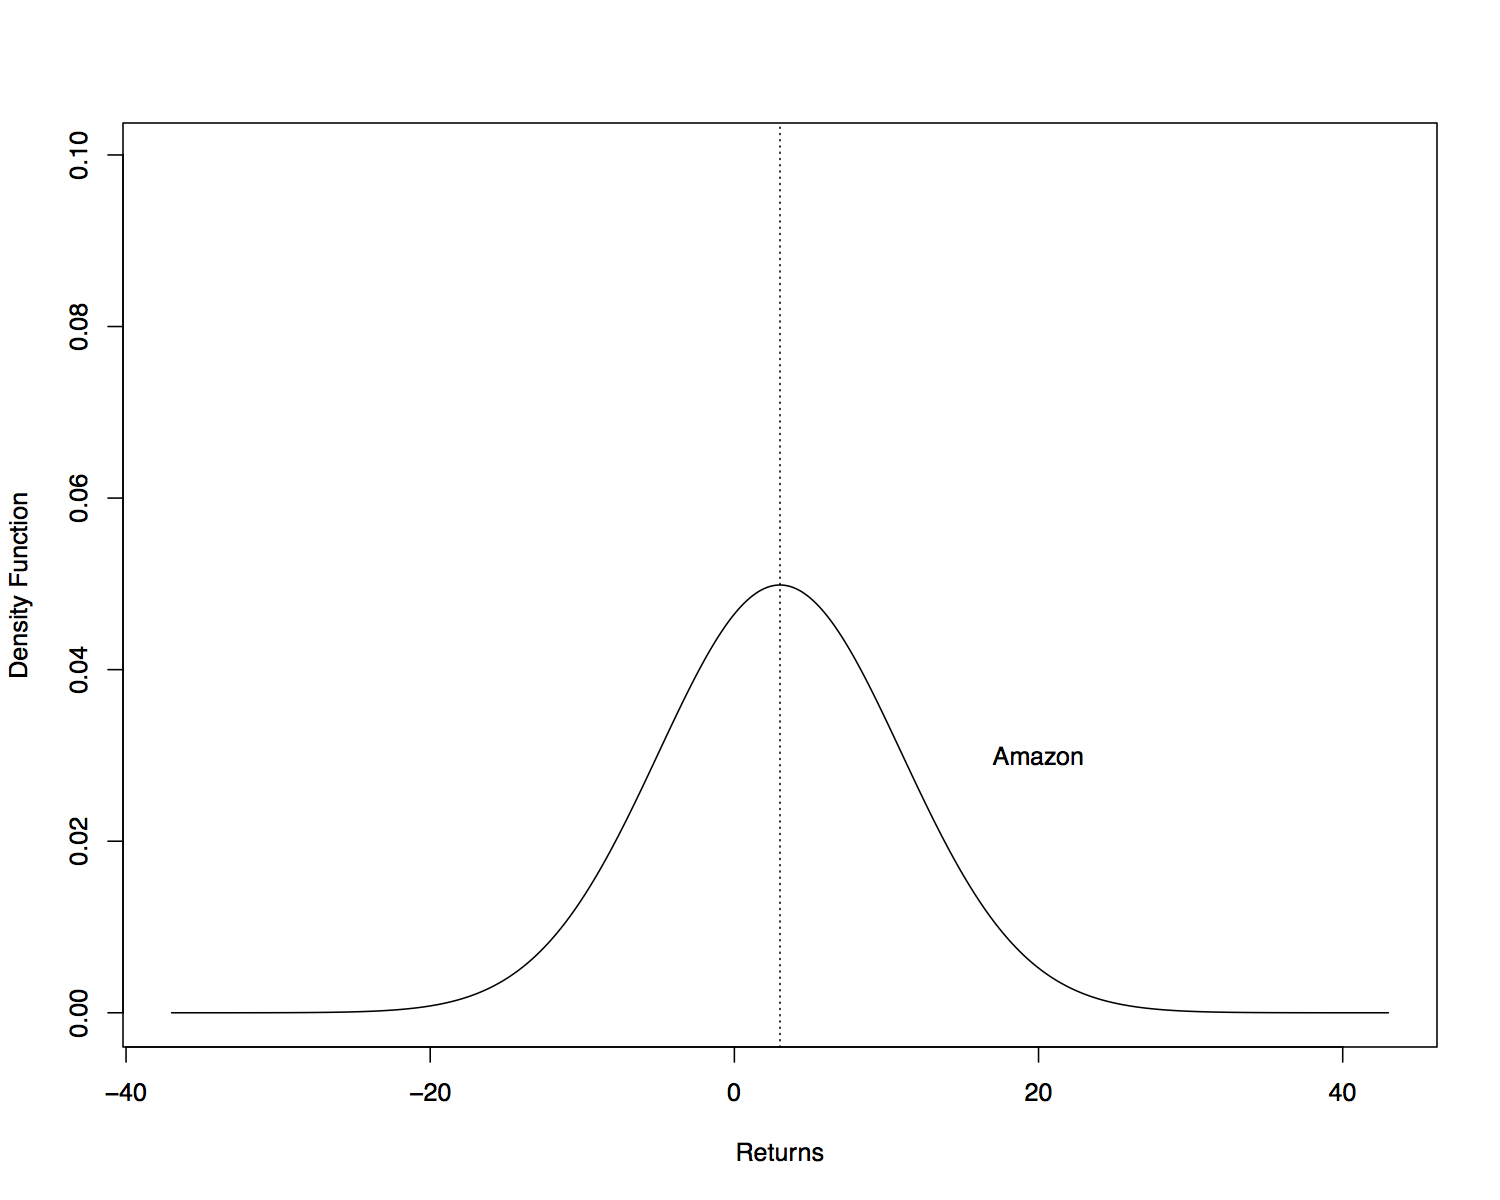
\includegraphics[width=6in]{amazon.png}


\subsection{Coca-Cola Distribution}
\label{risk:coca-cola-distribution}
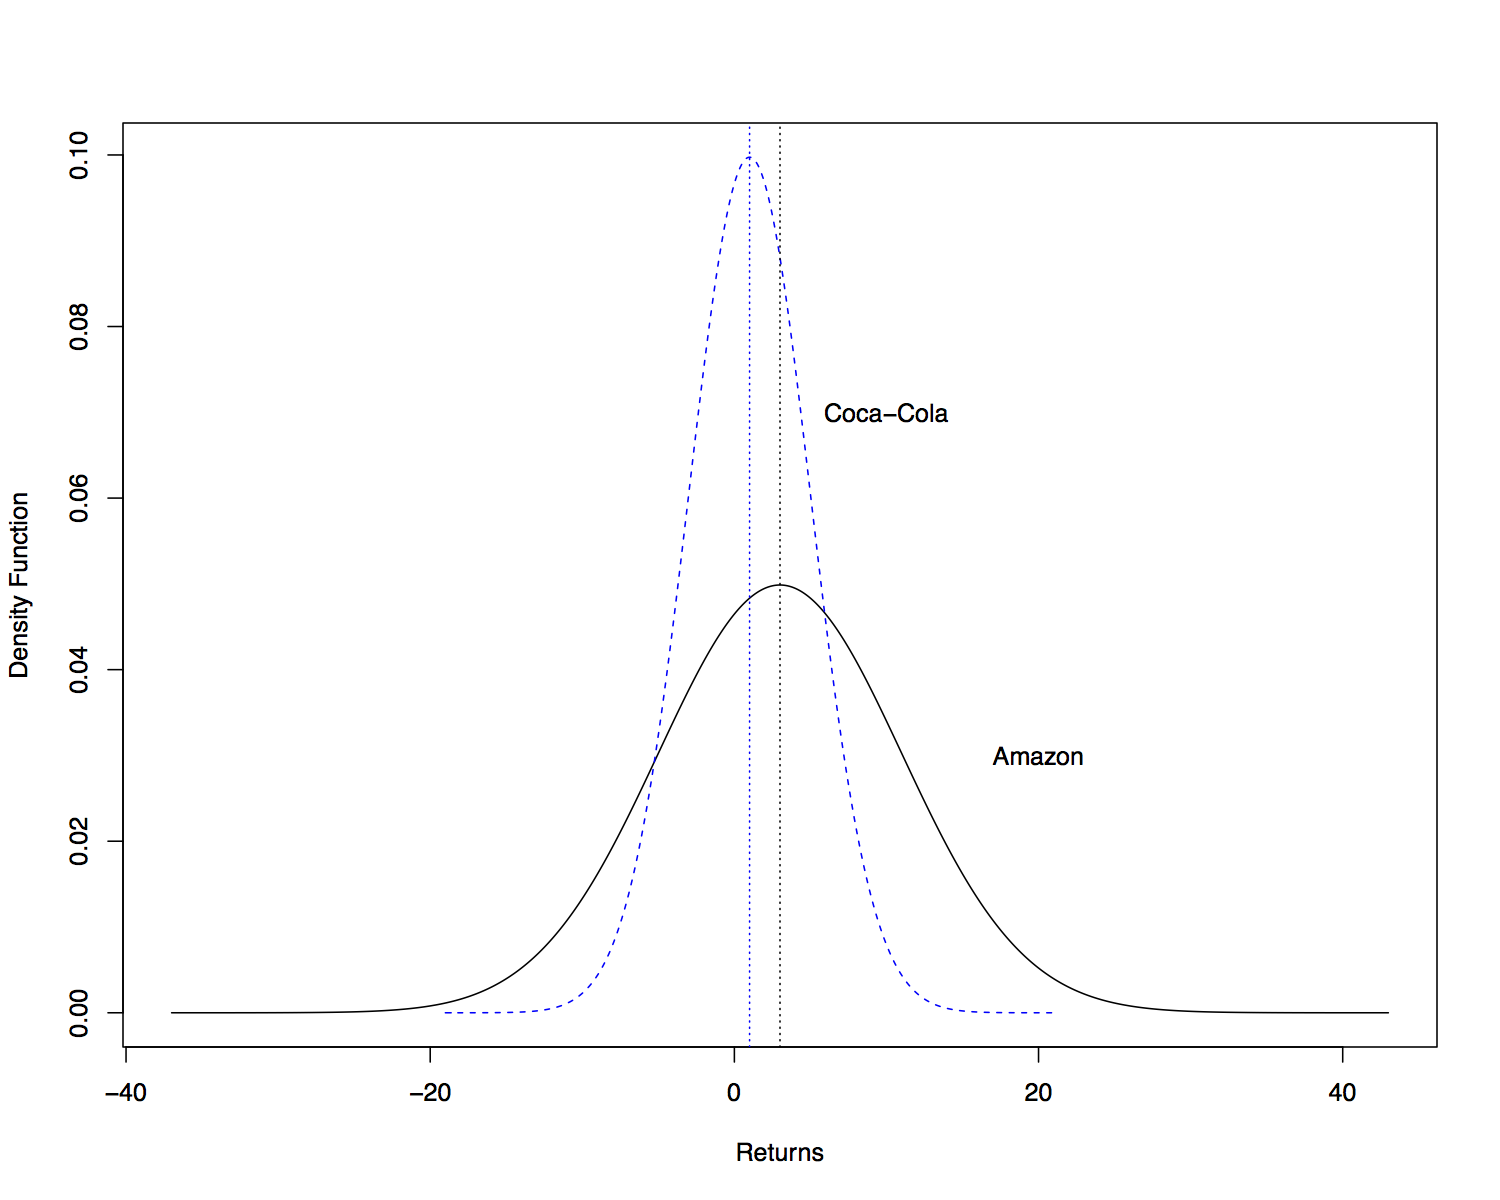
\includegraphics[width=6in]{amazon_coke.png}


\subsection{Implications of Normality}
\label{risk:implications-of-normality}
The assumption of normality is convenient because
\begin{itemize}
\item {} 
If we form a portfolio of assets that are normally distributed, then
the distribution of the portfolio return is also normally
distributed.
\begin{itemize}
\item {} 
Recall that if $X_i \sim \mathcal{N}(\mu_i, \sigma_i)$,
$i = 1,\ldots,N$, then $W = \sum_{i=1}^N w_i X_i$ is
also normally distributed (where $w_i$ are constant
weights).

\end{itemize}

\end{itemize}
\begin{itemize}
\item {} 
The mean and the variance (or standard deviation) fully characterize
the distribution of returns.

\end{itemize}
\begin{itemize}
\item {} 
The variance or standard deviation alone is an appropriate measure
of risk (no other measure is needed).

\end{itemize}


\subsection{Estimating Means and Volatilities}
\label{risk:estimating-means-and-volatilities}
Typically we don't know the true mean and standard deviation of Amazon
and Coca-Cola.  What do we do?
\begin{itemize}
\item {} 
Use historical data to estimate them.

\end{itemize}
\begin{itemize}
\item {} 
Collect $N+1$ past prices of each asset for a particular
interval of time (daily, monthly, quarterly, annually).

\end{itemize}
\begin{itemize}
\item {} 
Compute $N$ returns using the formula

\end{itemize}
\begin{gather}
\begin{split}r_t & = \frac{P_t - P_{t-1}}{P_{t-1}}.\end{split}\notag
\end{gather}
We don't include dividends in the return calculation above, because we
use ADJUSTED closing prices, which account for dividend payments
directly in the prices.


\subsection{Estimating Means and Volatilities}
\label{risk:id1}
Compute the sample mean of returns
\begin{gather}
\begin{split}\hat{\mu} & = \frac{1}{N} \sum_{t=1}^N r_t.\end{split}\notag
\end{gather}
Compute the sample standard deviation of returns
\begin{gather}
\begin{split}\hat{\sigma}^2 & = \frac{1}{N-1} \sum_{t=1}^N (r_t -
\hat{\mu})^2.\end{split}\notag
\end{gather}
The ``hats'' indicate that we have estimated $\mu$ and
$\sigma$: these are not the true, unknown values.


\subsection{Estimating Means and Volatilities - Example}
\label{risk:estimating-means-and-volatilities-example}
Let's collect the $N = 13$ closing prices for Amazon and
Coca-Cola between 3 Jan 2012 and 2 Jan 2013.
\begin{itemize}
\item {} 
We will only keep the first closing price on the first trading day
of each month.

\end{itemize}
\begin{itemize}
\item {} 
We can then compute 12 monthly returns by computing the difference
in month prices at the beginning of each month, dividing by the
price of the previous month.

\end{itemize}
\begin{itemize}
\item {} 
This will give us 12 returns that we can use to estimate the means
and standard deviations.

\end{itemize}


\subsection{Amazon Monthly Prices}
\label{risk:amazon-monthly-prices}
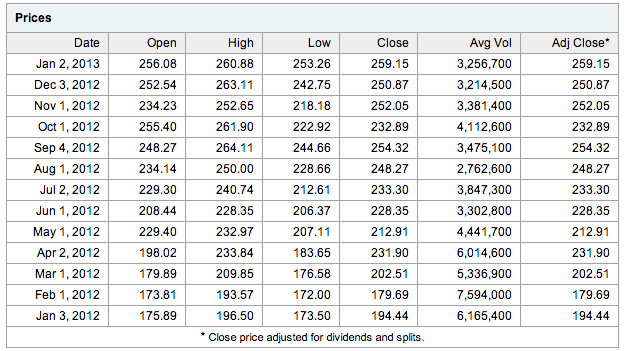
\includegraphics[width=6in]{amzn-monthly.png}


\subsection{Coca-Cola Monthly Prices}
\label{risk:coca-cola-monthly-prices}
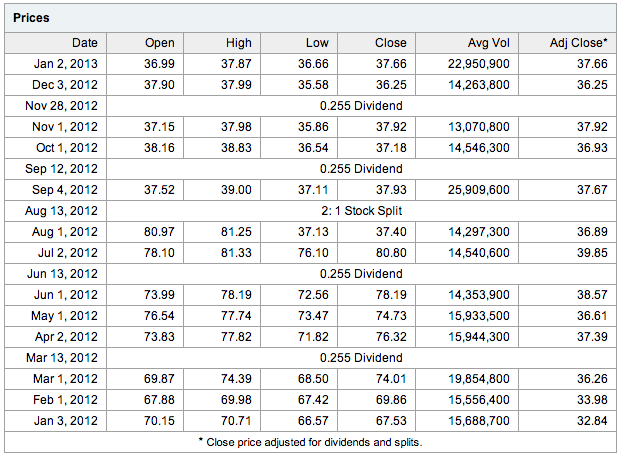
\includegraphics[width=6in]{ko-monthly.png}


\subsection{Computing Returns and Moments}
\label{risk:computing-returns-and-moments}
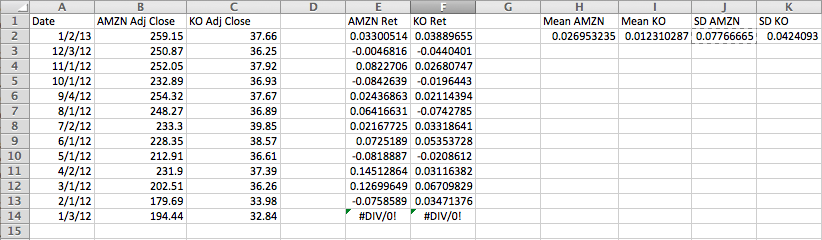
\includegraphics[width=6in]{amzn-coke-xls.png}


\subsection{Risk-Free Returns}
\label{risk:risk-free-returns}
We will typically assume that a risk-free asset is available for
purchase.
\begin{itemize}
\item {} 
We will denote the risk-free return as $r_f$.

\end{itemize}
\begin{itemize}
\item {} 
If an asset is risk free, its return is certain and has no
variability:

\end{itemize}
\begin{gather}
\begin{split}E[r_f] & = r_f \\
Var(r_f) & = 0.\end{split}\notag
\end{gather}

\subsection{T-Bills as Risk-Free Assets}
\label{risk:t-bills-as-risk-free-assets}
The return on a short-term government t-bill is usually considered
risk free:
\begin{itemize}
\item {} 
Although the price changes over time, the risk of default is
extremely low.

\end{itemize}
\begin{itemize}
\item {} 
Also, the holding period return can be determined at the beginning
of the holding period (unlike other risky assets).

\end{itemize}


\subsection{Compensation for Risk}
\label{risk:compensation-for-risk}
If you can invest in a risk-free asset, why would you purchase a
risky asset instead?
\begin{itemize}
\item {} 
Risky assets compensate for risk through higher expected
return.

\end{itemize}
\begin{itemize}
\item {} 
If risky assets didn't offer higher expected return, everyone would
sell them, leading to a price decline today and a higher expected
return:

\end{itemize}
\begin{gather}
\begin{split}\uparrow E[r_t] & = \frac{E[P_t] - \downarrow
P_{t-1}}{\downarrow P_{t-1}}\end{split}\notag
\end{gather}\begin{itemize}
\item {} 
There is no guarantee that the actual return will be higher -- only
its expected value.

\end{itemize}


\subsection{Risk Premium \& Excess Returns}
\label{risk:risk-premium-excess-returns}
The amount by which the expected return of some risky asset $A$
exceeds the risk-free return is known as the \emph{risk premium}:
\begin{gather}
\begin{split}\text{rp}_{A,t} & = E[r_{A,t}] - r_{f,t}.\end{split}\notag
\end{gather}
The \emph{excess return} measures the difference between a previously
observed holding period return of $A$ and the risk-free:
\begin{gather}
\begin{split}\text{er}_{A,t-1} & = r_{A,t-1} - r_{f,t-1}.\end{split}\notag
\end{gather}

\subsection{Risk Premium \& Excess Returns}
\label{risk:id2}\begin{itemize}
\item {} 
Note that excess returns can only be computed with past returns.

\end{itemize}
\begin{itemize}
\item {} 
We estimate risk premia with the sample mean of historical excess
returns.

\end{itemize}


\subsection{Sharpe Ratio}
\label{risk:sharpe-ratio}
The \emph{Sharpe Ratio} is a measure of how much risk premium investors
require, per unit of risk:
\begin{gather}
\begin{split}\text{SR}_{A,t} & = \frac{\mu_{A,t} - r_{f,t}}{\sigma_{A,t}}\end{split}\notag
\end{gather}\begin{itemize}
\item {} 
The Sharpe Ratio is a measure of risk aversion.

\end{itemize}
\begin{itemize}
\item {} 
It is often referred to as the price of risk.

\end{itemize}
\begin{itemize}
\item {} 
The Sharpe Ratio for a broad market index of assets (like the
S\&P 500) is referred to as the market price of risk.

\end{itemize}
\begin{itemize}
\item {} 
The true Sharpe Ratio is unknown, since we don't know
$\mu_{A,t}$ and $\sigma_{A,t}$, but we can estimate
these with historical returns.

\end{itemize}


\subsection{Risk Premium Example}
\label{risk:risk-premium-example}
Suppose the monthly risk-free rate is 0.2\%. What is the estimated
risk premium and Sharpe Ratio for Amazon stock?
\begin{gather}
\begin{split}rp_{AMZN} = 0.03 - 0.002 = 0.028\end{split}\notag
\end{gather}\begin{gather}
\begin{split}SR_{AMZN} = \frac{rp_{AMZN}}{0.08} = 0.35\end{split}\notag
\end{gather}

\chapter{Portfolio Optimization}
\label{portfolios:portfolio-optimization}\label{portfolios::doc}
Contents:


\section{Asset Allocation}
\label{allocation:asset-allocation}\label{allocation::doc}

\subsection{Utility}
\label{allocation:utility}
Investors usually care about maximizing utility.
\begin{itemize}
\item {} 
Suppose all investors have utility function

\end{itemize}
\begin{gather}
\begin{split}U(\mu, \sigma) & = \mu - \gamma \sigma^2.\end{split}\notag
\end{gather}\begin{itemize}
\item {} 
$\mu$ and $\sigma$ are the mean and standard deviation
of asset returns.

\end{itemize}
\begin{itemize}
\item {} 
What is the utility of holding a risk-free asset $U(\mu_f,
\sigma_f)$?

\end{itemize}
\begin{gather}
\begin{split}U(\mu_f ,\sigma_f) = r_f.\end{split}\notag
\end{gather}

\subsection{Certainty Equivalent}
\label{allocation:certainty-equivalent}
For a risky portfolio, $U(\mu_f, \sigma_f)$ can be thought of as
a certainty equivalent return.
\begin{itemize}
\item {} 
The return that a risk-free asset would have to offer to provide the
same utility level as a risky asset.

\end{itemize}


\subsection{Risk Aversion}
\label{allocation:risk-aversion}
The parameter $\gamma$ is a measure of risk
preference.
\begin{itemize}
\item {} 
If $\gamma > 0$ individuals are risk averse - volatility
detracts from utility.

\end{itemize}
\begin{itemize}
\item {} 
If $\gamma = 0$ individuals are risk neutral - volatility
doesn't enter into the utility function.
\begin{itemize}
\item {} 
In this case, investors rank portfolios by their expected return
and don't care about portfolio riskiness.

\end{itemize}

\end{itemize}


\subsection{Risk Aversion}
\label{allocation:id1}\begin{itemize}
\item {} 
If $\gamma < 0$ individuals are risk lovers - volatility is
rewarded in the utility function.
\begin{itemize}
\item {} 
In this case, investors enjoy and get utility by taking on risk.

\end{itemize}

\end{itemize}
\begin{itemize}
\item {} 
We will generally assume investors are risk averse, with the
magnitude of $\gamma$ dictating the amount of risk aversion.

\end{itemize}


\subsection{Mean-Variance Criterion}
\label{allocation:mean-variance-criterion}
Under this utility model, investors prefer higher expected returns
and lower volatility.
\begin{itemize}
\item {} 
Let portfolio $A$ have mean and volatility $\mu_A$ and
$\sigma_A$.

\end{itemize}
\begin{itemize}
\item {} 
Let portfolio $B$ have mean and volatility $\mu_B$ and
$\sigma_B$.

\end{itemize}
\begin{itemize}
\item {} 
If $\mu_A \geq \mu_B$ \emph{and} $\sigma_A \leq
\sigma_B$, then $A$ is preferred to $B$.

\end{itemize}


\subsection{Mean-Variance Criterion}
\label{allocation:id2}
$\qquad$

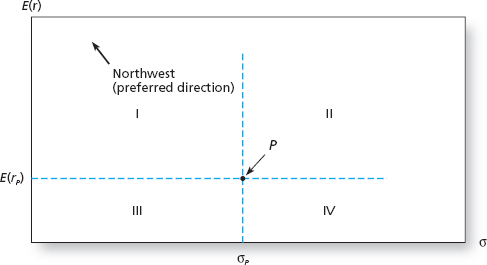
\includegraphics[width=6in]{pg164_1.jpg}


\subsection{Indifference Curves}
\label{allocation:indifference-curves}
Portfolios in quadrant I are preferred to $P$, which is preferred to
portfolios in quadrant IV.
\begin{itemize}
\item {} 
What about quadrants II and III?

\end{itemize}
\begin{itemize}
\item {} 
If a portfolio $Q$ has a mean and volatility that differ from
$P$ but yields the same utility level, then either

\end{itemize}
\begin{gather}
\begin{split}\mu_Q > \mu_p \text{  and  } \sigma_Q > \sigma_p\end{split}\notag
\end{gather}
or
\begin{gather}
\begin{split}\mu_Q < \mu_p \text{  and  } \sigma_Q < \sigma_p.\end{split}\notag
\end{gather}\begin{itemize}
\item {} 
That is, Q must be in quadrants II or III.

\end{itemize}


\subsection{Indifference Curves}
\label{allocation:id3}\begin{itemize}
\item {} 
The portfolios that yield the same utility as $P$ constitute
an indifference curve.

\end{itemize}
\begin{itemize}
\item {} 
We conclude that the indifference curve must cut through quadrants
II and III.

\end{itemize}


\subsection{Indifference Curve Plot}
\label{allocation:indifference-curve-plot}
$\qquad$

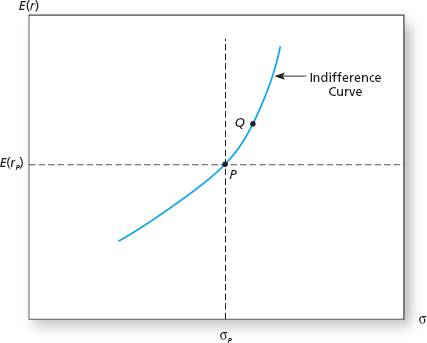
\includegraphics[width=6in]{pg165_2.jpg}


\subsection{Portfolios of Assets}
\label{allocation:portfolios-of-assets}
Suppose an individual can invest in two assets: a risky portfolio
$P$ and a risk-free asset $F$.
\begin{itemize}
\item {} 
$\omega$ will be the fraction wealth invested in
$P$.

\end{itemize}
\begin{itemize}
\item {} 
$1-\omega$ will be the fraction wealth invested in
$F$.

\end{itemize}
\begin{itemize}
\item {} 
We will typically assume that portfolio weights sum to
1.

\end{itemize}
\begin{itemize}
\item {} 
$r_p$ will denote the return on asset $P$, with
$\mu_p = E[r_p]$ and $\sigma_p^2 = Var(r_p)$.

\end{itemize}
\begin{itemize}
\item {} 
$r_f$ will denote the return on asset $F$, with
$\mu_f = r_f$ and $\sigma_f^2 = 0$.

\end{itemize}


\subsection{Portfolio Return}
\label{allocation:portfolio-return}
Let $C$ denote the portfolio that \emph{combines} the two assets.
\begin{itemize}
\item {} 
$C$ is a weighted average of $P$ and $F$:

\end{itemize}
\begin{gather}
\begin{split}C = \omega P + (1-\omega) F.\end{split}\notag
\end{gather}\begin{itemize}
\item {} 
The return to $C$, is

\end{itemize}
\begin{gather}
\begin{split}r_c = \omega r_p + (1-\omega) r_f.\end{split}\notag
\end{gather}

\subsection{Portfolio Return}
\label{allocation:id4}
By the linearity of expectations:
\begin{gather}
\begin{split}\mu_c = E[r_c] \qquad \qquad \qquad\end{split}\notag
\end{gather}\begin{gather}
\begin{split}\quad \enspace \, = \omega E[r_p] + (1 - \omega)E[r_f]\end{split}\notag
\end{gather}\begin{gather}
\begin{split}= \omega \mu_p + (1-\omega) r_f \enspace \,\end{split}\notag
\end{gather}\begin{gather}
\begin{split}= r_f + \omega(\mu_p - r_f). \enspace \,\end{split}\notag
\end{gather}\begin{itemize}
\item {} 
The term in the parentheses is the risk premium of $P$.

\end{itemize}


\subsection{Portfolio Volatility}
\label{allocation:portfolio-volatility}
According to the properties of variance,
\begin{gather}
\begin{split}\sigma^2_c = Var(r_c) \qquad \qquad \qquad \qquad \qquad \qquad
\qquad \qquad \enspace\end{split}\notag
\end{gather}\begin{gather}
\begin{split}\quad \enspace \; \, = \omega^2 Var(r_p) + (1 - \omega)^2 Var(r_f) + 2
\omega (1 - \omega) Cov(r_p, r_f)\end{split}\notag
\end{gather}\begin{gather}
\begin{split}= \omega^2 Var(r_p) \qquad \qquad \qquad \qquad \qquad \qquad
\quad \enspace \; \: \,\end{split}\notag
\end{gather}\begin{gather}
\begin{split}= \omega^2 \sigma^2_p. \qquad \qquad \qquad \qquad \qquad \qquad
\qquad \quad \enspace \; \,\end{split}\notag
\end{gather}\begin{itemize}
\item {} 
The third equality follows because $r_f$ is a constant.

\end{itemize}
\begin{itemize}
\item {} 
Thus,

\end{itemize}
\begin{gather}
\begin{split}\sigma_c = \omega \sigma_p.\end{split}\notag
\end{gather}

\subsection{Portfolios and Risk Aversion}
\label{allocation:portfolios-and-risk-aversion}
Portfolio $C$ earns a base return of $r_f$ plus the risk
premium associated with $P$, weighted by the amount of wealth
the investor allocates to $P$.
\begin{itemize}
\item {} 
More risk averse investors (small $\omega$) expect a rate of
return closer to $r_f$.

\end{itemize}
\begin{itemize}
\item {} 
Less risk averse investors (high $\omega$) expect a rate
closer to $\mu_p - r_f$.

\end{itemize}
\begin{itemize}
\item {} 
More risk averse investors have smaller portfolio volatilities.

\end{itemize}
\begin{itemize}
\item {} 
Less risk averse investors have higher portfolio volatilities.

\end{itemize}


\subsection{Portfolio Weight}
\label{allocation:portfolio-weight}
Since $\sigma_c = \omega \sigma_p$,
\begin{gather}
\begin{split}\omega =\frac{\sigma_c}{\sigma_p}.\end{split}\notag
\end{gather}

\subsection{Sharpe Ratio}
\label{allocation:sharpe-ratio}
Thus
\begin{gather}
\begin{split}\mu_c = r_f + \omega (\mu_p - r_f) \qquad\end{split}\notag
\end{gather}\begin{gather}
\begin{split}= r_f + \frac{\sigma_c}{\sigma_p} (\mu_p - r_f) \:\end{split}\notag
\end{gather}\begin{gather}
\begin{split}= r_f + \frac{\mu_p - r_f}{\sigma_p} \sigma_c \enspace \; \,\end{split}\notag
\end{gather}\begin{gather}
\begin{split}= r_f + \text{SR}_p \sigma_c. \qquad \enspace\end{split}\notag
\end{gather}\begin{itemize}
\item {} 
$\text{SR}_p$ is the Sharpe Ratio of portfolio $P$.

\end{itemize}


\subsection{Capital Allocation Line}
\label{allocation:capital-allocation-line}
The Capital Allocation Line (CAL) depicts the set of portfolios
available to an investor (a budget constraint).
\begin{itemize}
\item {} 
It plots pairs of $\sigma_c$ and $\mu_c$ that the
investor can choose by selecting $\omega$.

\end{itemize}
\begin{itemize}
\item {} 
This is simply a plot of the equation

\end{itemize}
\begin{gather}
\begin{split}\mu_c = r_f + \text{SR}_p \sigma_c.\end{split}\notag
\end{gather}\begin{itemize}
\item {} 
Clearly, the intercept will be $r_f$ and the slope will be
$\text{SR}_p$.

\end{itemize}


\subsection{Capital Allocation Line Example}
\label{allocation:capital-allocation-line-example}
Suppose
\begin{itemize}
\item {} 
$r_f = 0.07$.

\end{itemize}
\begin{itemize}
\item {} 
$\mu_p = 0.15$.

\end{itemize}
\begin{itemize}
\item {} 
$\sigma_p = 0.22$.

\end{itemize}

What is the CAL?


\subsection{Capital Allocation Line Plot}
\label{allocation:capital-allocation-line-plot}
$\qquad$

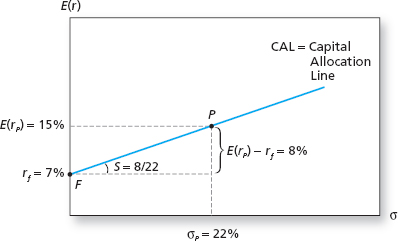
\includegraphics[width=6in]{pg172_1.jpg}


\subsection{Simple Portfolio Choice}
\label{allocation:simple-portfolio-choice}
Individuals seek to maximize utility subject to the available choice
set.
\begin{gather}
\begin{split}\max_{\mu_c, \sigma_c} U(\mu_c, \sigma_c) = \max_{\mu_c, \sigma_c}
\mu_c - \frac{1}{2} \gamma \sigma^2_c,\end{split}\notag
\end{gather}
subject to
\begin{gather}
\begin{split}\mu_c & = r_f + \omega (\mu_p - r_f) \\
\sigma_c & = \omega \sigma_p.\end{split}\notag
\end{gather}

\subsection{Simple Portfolio Choice (Cont.)}
\label{allocation:simple-portfolio-choice-cont}
Substituting the constraints, the maximization problem becomes
\begin{gather}
\begin{split}\max_{\omega} \left\{r_f + \omega (\mu_p - r_f) - \frac{1}{2}
\gamma \omega^2 \sigma^2_p \right\}.\end{split}\notag
\end{gather}
Taking the derivative of this equation w.r.t. $\omega$,
\begin{gather}
\begin{split}\mu_p - r_f  = \gamma \omega^* \sigma^2_p\end{split}\notag
\end{gather}\begin{gather}
\begin{split}\Rightarrow \omega^* = \frac{\mu_p - r_f}{\gamma \sigma^2_p} =
\frac{\text{SR}_p}{\gamma \sigma_p}.\end{split}\notag
\end{gather}

\subsection{Simple Portfolio Choice}
\label{allocation:id5}
Since the CAL is a choice set (budget constraint), we can find the
optimal portfolio by observing where an indifference curve is
tangent to the CAL.
\begin{itemize}
\item {} 
Fix the utility value at $\bar{U} = r_f$.

\end{itemize}
\begin{itemize}
\item {} 
Use the relation $\bar{U} = \mu_c - \frac{1}{2} \gamma
\sigma^2_c$ to solve for $\mu_c$:

\end{itemize}
\begin{gather}
\begin{split}\mu_c = \bar{U} + \frac{1}{2} \gamma \sigma^2_c.\end{split}\notag
\end{gather}

\subsection{Simple Portfolio Choice}
\label{allocation:id6}\begin{itemize}
\item {} 
Using this equation, we find the pairs of $\mu_c$ and
$\sigma_c$ that corresponds to utility $\bar{U}$, which we
plot.

\end{itemize}
\begin{itemize}
\item {} 
Repeat this process, increasing the values of $\bar{U}$ until a
tangent indifference curve is found. The tangency corresponds to
the optimal portfolio.

\end{itemize}


\subsection{Spreadsheet Optimization}
\label{allocation:spreadsheet-optimization}
Given $\gamma=2$, $\mu=0.15$, $\sigma=0.22$ and
$r_f=0.07$.

$\qquad$

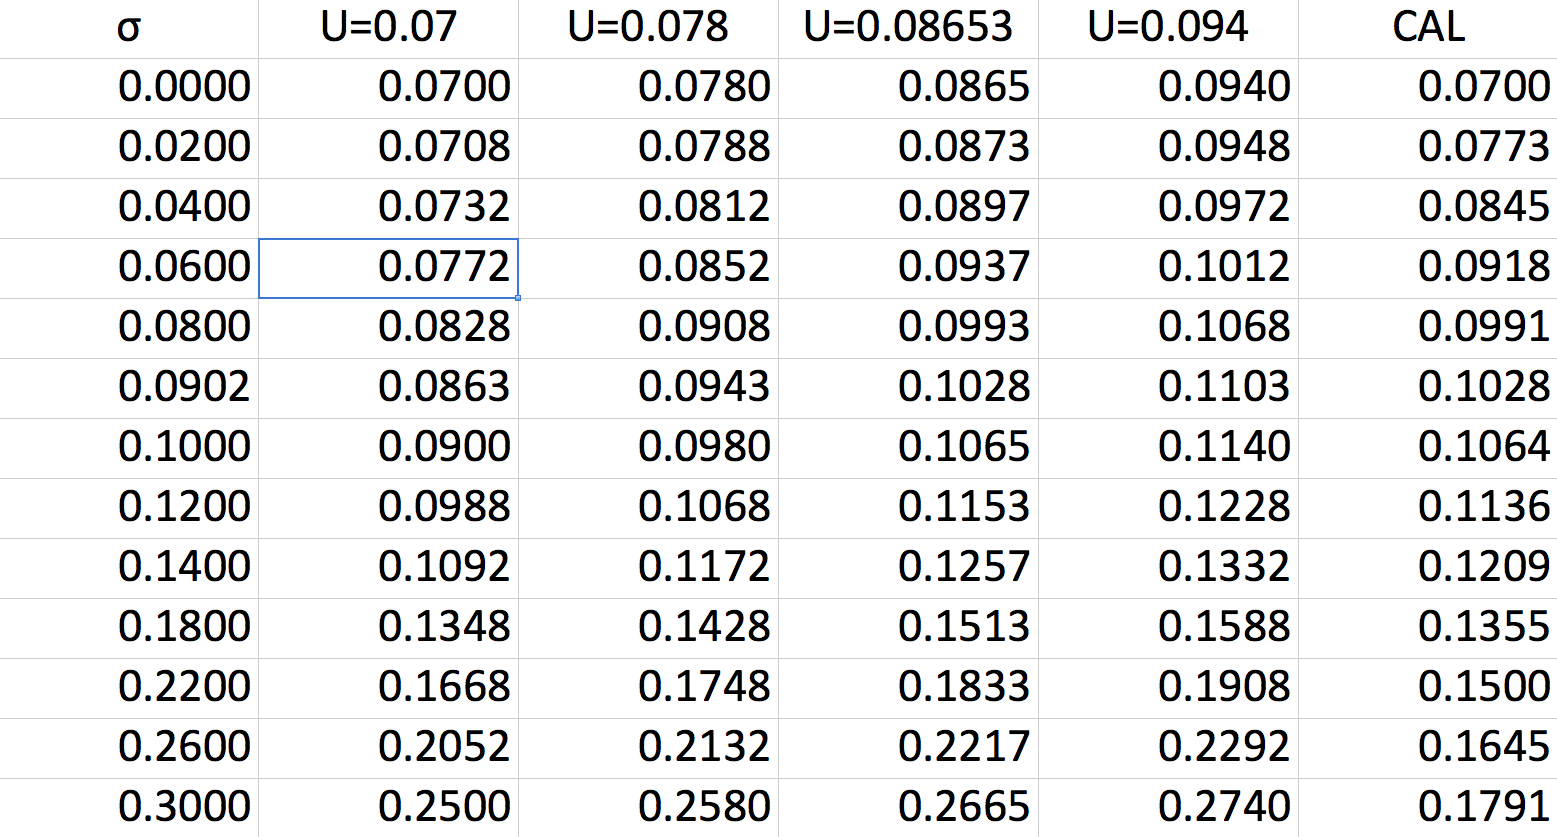
\includegraphics[width=6in]{calSS.png}


\subsection{Graphical Optimization}
\label{allocation:graphical-optimization}
$\qquad$

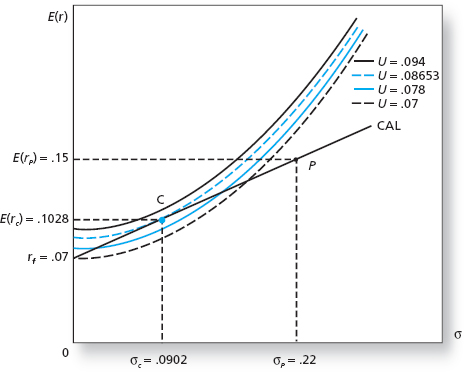
\includegraphics[width=6in]{pg177_2.jpg}


\subsection{Capital Market Line}
\label{allocation:capital-market-line}
Consider a value-weighted portfolio of all assets in the
market.
\begin{itemize}
\item {} 
We will call this the market portfolio and denote it by
$M$.

\end{itemize}
\begin{itemize}
\item {} 
The CAL which connects $r_f$ with $M$ is called the
\emph{Capital Market Line} (CML).

\end{itemize}
\begin{itemize}
\item {} 
Because the true market portfolio is unobserved, we use a
proxy - a well diversified portfolio that provides a good
representation of the entire market.

\end{itemize}
\begin{itemize}
\item {} 
Typically we use the S\&P 500.

\end{itemize}


\subsection{Passive vs. Active Strategies}
\label{allocation:passive-vs-active-strategies}
Holding the market portfolio or a market proxy is known as a \emph{passive
strategy}.
\begin{itemize}
\item {} 
It requires no security analysis.

\end{itemize}
\begin{itemize}
\item {} 
An \emph{active strategy} is one that requires individual security
analysis.

\end{itemize}


\section{Portfolio Optimization}
\label{portfolioOpt:portfolio-optimization}\label{portfolioOpt::doc}

\subsection{Types of Risk}
\label{portfolioOpt:types-of-risk}
We classify risk using two broad categories.
\begin{itemize}
\item {} 
Systematic risk (also called market or non-diversifiable risk) which
is common to all assets in the market.

\end{itemize}
\begin{itemize}
\item {} 
Idiosyncratic risk (also called firm-specific, non-systematic or
diversifiable risk) which is unique to a particular asset.

\end{itemize}


\subsection{Benefits of Diversification}
\label{portfolioOpt:benefits-of-diversification}
Idiosyncratic risk can be eliminated through portfolio
diversification.
\begin{itemize}
\item {} 
Imagine holding one stock in your portfolio. The risk of your
portfolio will be equal to the sum of the stock's systematic and
idiosyncratic risks.

\end{itemize}
\begin{itemize}
\item {} 
Now add another stock to the portfolio. If the two stocks are
perfectly correlated, then they will always move together and your
portfolio will have the same risk properties as before.

\end{itemize}


\subsection{Benefits of Diversification}
\label{portfolioOpt:id1}\begin{itemize}
\item {} 
What if the idiosyncratic components of the two stocks are
uncorrelated?
\begin{itemize}
\item {} 
Systematic shocks will cause them to move together.

\end{itemize}
\begin{itemize}
\item {} 
Idiosyncratic shocks will occur at different times and magnitudes,
so the stocks will not move together as much.

\end{itemize}
\begin{itemize}
\item {} 
Sometimes when one falls in price another will rise price,
counteracting each other and reducing risk.

\end{itemize}

\end{itemize}


\subsection{Benefits of Diversification}
\label{portfolioOpt:id2}\begin{itemize}
\item {} 
What if the idiosyncratic components of the two stocks are
negatively correlated?
\begin{itemize}
\item {} 
Systematic shocks will cause them to move together.

\end{itemize}
\begin{itemize}
\item {} 
Idiosyncratic shocks will cause them to move in opposite
directions, reducing risk.

\end{itemize}

\end{itemize}


\subsection{Limits to Diversification}
\label{portfolioOpt:limits-to-diversification}
Adding more and more assets to a portfolio compounds the
diversification effect.
\begin{itemize}
\item {} 
In theory, it should be possible to eliminate all idiosyncratic risk
by increasing the number of assets in a portfolio.

\end{itemize}
\begin{itemize}
\item {} 
Systematic risk, however, cannot be eliminated since it is common to
all assets.

\end{itemize}


\subsection{Limits to Diversification}
\label{portfolioOpt:id3}
$\qquad$

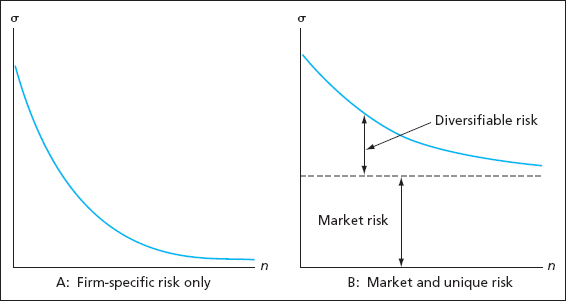
\includegraphics[width=6in]{bod34698_0601_lg.jpg}


\subsection{Portfolios of Two Risky Assets}
\label{portfolioOpt:portfolios-of-two-risky-assets}
Suppose you can invest in two risky assets.
\begin{itemize}
\item {} 
A debt asset (bonds) denoted by $D$.

\end{itemize}
\begin{itemize}
\item {} 
An equity asset (stocks) denoted by $E$.

\end{itemize}
\begin{itemize}
\item {} 
$\omega_d$ is the fraction of wealth invested in $D$.

\end{itemize}
\begin{itemize}
\item {} 
$\omega_e$ is the fraction of wealth invested in $E$.

\end{itemize}
\begin{itemize}
\item {} 
We require $\omega_d + \omega_e = 1$, so that $\omega_e
= 1 - \omega_d$.

\end{itemize}


\subsection{Returns to Portfolios of Risky Assets}
\label{portfolioOpt:returns-to-portfolios-of-risky-assets}
Suppose the returns to $D$ and $E$ are $r_d$ and
$r_e$, respectively.
\begin{itemize}
\item {} 
The portfolio return is the weighted average of returns

\end{itemize}
\begin{gather}
\begin{split}r_p  = \omega_d r_d + \omega_e r_e.\end{split}\notag
\end{gather}\begin{itemize}
\item {} 
By the properties of expectations, the portfolio expected return is

\end{itemize}
\begin{gather}
\begin{split}\mu_p = \omega_d \mu_d + \omega_e \mu_e.\end{split}\notag
\end{gather}\begin{itemize}
\item {} 
By the properties of variance, the portfolio variance is

\end{itemize}
\begin{gather}
\begin{split}\sigma^2_p = \omega^2_d \sigma^2_d + \omega^2_e \sigma^2_e + 2
\omega_d \omega_e Cov(r_d, r_e).\end{split}\notag
\end{gather}

\subsection{Covariance Matrix}
\label{portfolioOpt:covariance-matrix}
It is often useful to express the variance and covariance information
in matrix form
\begin{gather}
\begin{split}\Sigma = \left[\begin{array}{cc} \sigma^2_d & \sigma_{d,e}
      \\ \sigma_{e,d} & \sigma^2_e \end{array} \right],\end{split}\notag
\end{gather}
where $\sigma_{d,e} = \sigma_{e,d} = Cov(r_d, r_e)$.
\begin{itemize}
\item {} 
$\Sigma$ is referred to as a covariance matrix.

\end{itemize}
\begin{itemize}
\item {} 
It can be generalized to more than two assets.

\end{itemize}
\begin{itemize}
\item {} 
The diagonal terms always represent variances.

\end{itemize}
\begin{itemize}
\item {} 
The off-diagonal terms represent covariances.

\end{itemize}


\subsection{Correlation}
\label{portfolioOpt:correlation}
Define $\rho_{xy} = Corr(X,Y)$.  Then recall that
\begin{gather}
\begin{split}\rho_{xy} = \frac{Cov(X,Y)}{\sigma_x \sigma_y}.\end{split}\notag
\end{gather}\begin{itemize}
\item {} 
Hence, $Cov(X,Y) = \rho_{xy} \sigma_x \sigma_y$.

\end{itemize}
\begin{itemize}
\item {} 
Remember that $\rho_{xy} \in [-1,1]$.

\end{itemize}


\subsection{Portfolio Variance}
\label{portfolioOpt:portfolio-variance}
The previous relationship allows us to write portfolio variance as
\begin{gather}
\begin{split}\sigma^2_p & = \omega^2_d \sigma^2_d + \omega^2_e \sigma^2_e + 2
\omega_d \omega_e \rho_{de} \sigma_d \sigma_e.\end{split}\notag
\end{gather}\begin{itemize}
\item {} 
Since $\rho_{de} \in [-1,1]$, $\sigma^2_p$ is greatest
when $\rho_{de} = 1$.  Why?

\end{itemize}
\begin{itemize}
\item {} 
Note that when $\rho_{de} = 1$,

\end{itemize}
\begin{gather}
\begin{split}\sigma^2_p = (\omega_d \sigma_d + \omega_e \sigma_e)^2\end{split}\notag
\end{gather}\begin{gather}
\begin{split}\Rightarrow \sigma_p = \omega_d \sigma_d + \omega_e \sigma_e.\end{split}\notag
\end{gather}

\subsection{Portfolio Standard Deviation}
\label{portfolioOpt:portfolio-standard-deviation}\begin{itemize}
\item {} 
In this special case, the portfolio standard deviation is the
weighted average of asset standard deviations.

\end{itemize}
\begin{itemize}
\item {} 
So the maximal possible portfolio standard deviation is the
simple weighted average of component standard deviations.

\end{itemize}


\subsection{Portfolio Variance}
\label{portfolioOpt:id4}
Note that
\begin{itemize}
\item {} 
$\mu_p$ is the weighted average of asset means.

\end{itemize}
\begin{itemize}
\item {} 
$\sigma_p$ is less than the weighted average of asset
volatilities when $\rho_{de} \neq 1$.

\end{itemize}
\begin{itemize}
\item {} 
So the risk-return properties of the portfolio are better than those
of the component assets.

\end{itemize}


\subsection{Portfolio Variance Lower Bound}
\label{portfolioOpt:portfolio-variance-lower-bound}
Portfolio variance is made smaller with smaller values of
$\rho_{de}$.
\begin{itemize}
\item {} 
When $\rho_{de} = -1$,

\end{itemize}
\begin{gather}
\begin{split}\sigma^2_p = (\omega_d \sigma_d - \omega_e \sigma_e)^2\end{split}\notag
\end{gather}\begin{gather}
\begin{split}\Rightarrow \sigma_p = |\omega_d \sigma_d - \omega_e \sigma_e|.\end{split}\notag
\end{gather}\begin{itemize}
\item {} 
If we choose $\omega_d = \frac{\sigma_e}{\sigma_e + \sigma_d}$
(and $\omega_e = 1-\omega_d$) then $\sigma_p = 0$.

\end{itemize}
\begin{itemize}
\item {} 
This means that if assets are perfectly negatively correlated, the
portfolio has zero variance.

\end{itemize}


\subsection{Portfolio Variance Lower Bound}
\label{portfolioOpt:id5}
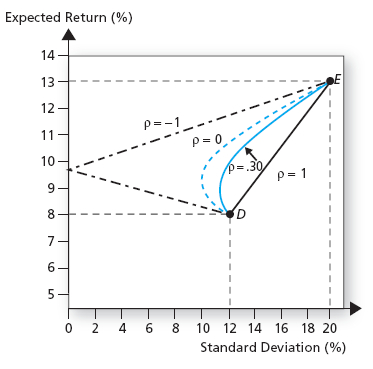
\includegraphics[width=6in]{pg205_1.jpg}


\subsection{Portfolio Frontier}
\label{portfolioOpt:portfolio-frontier}
The lines in the figure above are known as \emph{portfolio opportunity
sets} or \emph{portfolio frontiers}.
\begin{itemize}
\item {} 
Since individuals prefer less risk and greater return, frontiers
that are bowed to the northwest are better.

\end{itemize}
\begin{itemize}
\item {} 
Clearly, the frontiers are better for smaller values of
$\rho_{de}$.

\end{itemize}


\subsection{Portfolios of Three Assets}
\label{portfolioOpt:portfolios-of-three-assets}
Assume you can invest your money in three assets:
\begin{itemize}
\item {} 
Two risky assets.

\end{itemize}
\begin{itemize}
\item {} 
A risk-free asset.

\end{itemize}

The portfolio frontier now consists of
\begin{itemize}
\item {} 
The curved frontier between the two risky assets. We will call this
the \emph{risky frontier}.

\end{itemize}
\begin{itemize}
\item {} 
Every capital allocation line (CAL) connecting the risk-free to a
portfolio on the risky frontier.

\end{itemize}
\begin{itemize}
\item {} 
Steeper CALs are better since they offer portfolios of equivalent
expected return with lower standard deviation.

\end{itemize}


\subsection{Efficient Frontier}
\label{portfolioOpt:efficient-frontier}
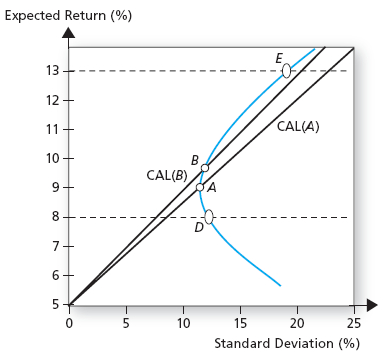
\includegraphics[width=6in]{pg206_1.jpg}


\subsection{Optimal CAL}
\label{portfolioOpt:optimal-cal}
The optimal CAL is the steepest possible line that intersects both the
risk-free asset and a portfolio on the risky frontier.
\begin{itemize}
\item {} 
The slope of the CAL is the Sharpe Ratio of the risky portfolio it
intersects.

\end{itemize}
\begin{itemize}
\item {} 
So the investor's optimization problem is

\end{itemize}
\begin{gather}
\begin{split}\max_{\omega} SR_p = \frac{\mu_p - r_f}{\sigma_p} \quad \text{subject to}\end{split}\notag
\end{gather}\begin{gather}
\begin{split}\mu_p = \omega_d \mu_d + (1-\omega_d) \mu_e\end{split}\notag
\end{gather}\begin{gather}
\begin{split}\sigma_p = \sqrt{\omega^2_d \sigma^2_d + (1-\omega_d)^2
\sigma^2_e + 2 \omega_d (1-\omega_d) \rho_{de} \sigma_d
\sigma_e}.\end{split}\notag
\end{gather}

\subsection{Optimal CAL}
\label{portfolioOpt:id6}
To solve the problem we
\begin{itemize}
\item {} 
Substitute the constraints.

\end{itemize}
\begin{itemize}
\item {} 
Take the derivative with respect to $\omega_d$ and set the
derivative equal to zero.

\end{itemize}
\begin{itemize}
\item {} 
Perform some tedious algebra.

\end{itemize}


\subsection{Optimal CAL}
\label{portfolioOpt:id7}
The solution is
\begin{gather}
\begin{split}\omega_d^* & = \frac{rp_d \sigma^2_e - rp_e
\rho_{de} \sigma_d \sigma_e}{rp_e \sigma^2_d +
rp_d \sigma^2_e - (rp_e + rp_d) \rho_{de}
\sigma_d \sigma_e}.\end{split}\notag
\end{gather}\begin{itemize}
\item {} 
$rp_d = \mu_d - r_f$ and $rp_e = \mu_e - r_f$.

\end{itemize}
\begin{itemize}
\item {} 
The optimal portfolio $T$ is known as the \emph{tangency
portfolio}.

\end{itemize}


\subsection{Tangeny Portfolio}
\label{portfolioOpt:tangeny-portfolio}
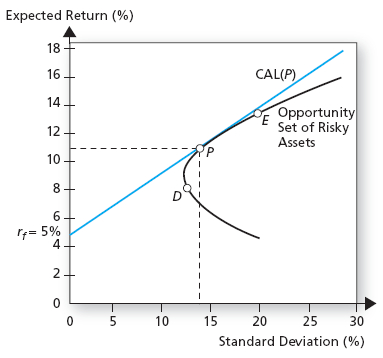
\includegraphics[width=6in]{pg208_1.jpg}


\subsection{Optimal CAL}
\label{portfolioOpt:id8}
The optimal CAL is the investor's efficient choice set, since it
offers minimal variance portfolios for every choice of expected
return.
\begin{itemize}
\item {} 
We have said nothing about which portfolio the investor will
actually consume; we have only identified the set from which the
investor will choose.

\end{itemize}
\begin{itemize}
\item {} 
We must combine the optimal CAL with a specification of preferences
to determine the investor's actual choice.

\end{itemize}
\begin{itemize}
\item {} 
The portfolio choice problem with three assets now reduces to the
simple problem of choosing between one risky asset (the tangency
portfolio) and the risk-free asset.

\end{itemize}


\subsection{Investor Choice}
\label{portfolioOpt:investor-choice}
Let's assume again that agents' utility is given by
\begin{gather}
\begin{split}U(\mu, \sigma) & = \mu - \frac{1}{2} \gamma \sigma^2.\end{split}\notag
\end{gather}
Recall that when allocating wealth between a risky asset $P$ and
a risk-free asset, the optimal portfolio weight, $\tau$, is
\begin{gather}
\begin{split}\tau & = \frac{\mu_p - r_f}{\gamma \sigma^2_p}.\end{split}\notag
\end{gather}

\subsection{Investor Choice}
\label{portfolioOpt:id9}
If the agent invests in the tangency portfolio $T$ and the
risk-free,
\begin{gather}
\begin{split}\tau = \frac{\mu_T - r_f}{\gamma  \sigma^2_T}.\end{split}\notag
\end{gather}\begin{itemize}
\item {} 
Given that the tangency portfolio is a weighted average of assets
$D$ and $E$, with optimal weight $\omega_d^*$

\end{itemize}
\begin{gather}
\begin{split}w_d & = \tau \omega_d^* \\
w_e & = \tau (1-\omega_d^*).\end{split}\notag
\end{gather}

\section{Portfolio Optimization with Many Risky Assets}
\label{multiAssetOpt:portfolio-optimization-with-many-risky-assets}\label{multiAssetOpt::doc}

\subsection{Portfolio Returns}
\label{multiAssetOpt:portfolio-returns}
Suppose you can now invest in an arbitrary number ($N$) of risky
assets.
\begin{itemize}
\item {} 
Index the assets by $i = 1, \ldots, N$.

\end{itemize}
\begin{itemize}
\item {} 
Let $\omega_i$ be the fraction of income invested in asset $i$.

\end{itemize}
\begin{itemize}
\item {} 
We will always assume that $\sum_{i=1}^N \omega_i = 1$.

\end{itemize}
\begin{itemize}
\item {} 
We will denote the return to asset $i$ by $r_i$.

\end{itemize}
\begin{itemize}
\item {} 
The portfolio return is expressed as

\end{itemize}
\begin{gather}
\begin{split}r_p = \sum_{i=1}^N \omega_i r_i.\end{split}\notag
\end{gather}

\subsection{Portfolio Moments}
\label{multiAssetOpt:portfolio-moments}
From the properties of expectation and variance, we can compute the
mean and variance of the portfolio return.
\begin{itemize}
\item {} 
Recognize that the $N$ asset returns, $r_i$, are random
variables.

\end{itemize}
\begin{itemize}
\item {} 
Denote the means of $r_i$ as $\mu_i$.

\end{itemize}


\subsection{Portfolio Moments}
\label{multiAssetOpt:id1}\begin{itemize}
\item {} 
The $N \times N$ covariance matrix of the returns contains the
variances, $\sigma^2_i$, and covariances, $Cov(r_i,
r_j) = \sigma_{ij}$:

\end{itemize}
\begin{gather}
\begin{split}\Sigma_P & = \left[\begin{array}{cccc} \sigma^2_1 &
\sigma_{12} & \cdots & \sigma_{1N} \\ \sigma_{21} &
\sigma^2_2 & \cdots & \sigma_{2N} \\ \vdots & \vdots &
\ddots & \vdots \\ \sigma_{N1} & \sigma_{N2} & \cdots &
\sigma^2_N \end{array}\right]\end{split}\notag
\end{gather}

\subsection{Portfolio Moments}
\label{multiAssetOpt:id2}
Thus resulting moments of the portfolio are
\begin{gather}
\begin{split}\mu_p & = \sum_{i=1}^N \omega_i \mu_i \\\end{split}\notag
\end{gather}\begin{gather}
\begin{split}\sigma^2_p & = \sum_{i=1}^N \omega^2_i \sigma^2_i +
2 \sum_{i=1}^{N-1} \sum_{j=i+1}^N \omega_i \omega_j \sigma_{ij}.\end{split}\notag
\end{gather}
What are other ways to express $\sigma^2_p$?


\subsection{Optimization: Risky MV Frontier}
\label{multiAssetOpt:optimization-risky-mv-frontier}
To determine the set of efficient risky portfolios (the risky
frontier), the investor solves
\begin{gather}
\begin{split}\min_{\{\omega_i\}_{i=1}^{N-1}} \sigma^2_P =
\sum_{i=1}^N \omega^2_i \sigma^2_i + 2 \sum_{i=1}^{N-1}
\sum_{j=i+1}^N \omega_i \omega_j \sigma_{ij}\end{split}\notag
\end{gather}
subject to
\begin{gather}
\begin{split}\mu_p = \sum_{i=1}^N \omega_i \mu_i\end{split}\notag
\end{gather}
where $\mu_p$ is some prespecified value of the portfolio mean
return.


\subsection{Optimization: Risky MV Frontier}
\label{multiAssetOpt:id3}
Note that
\begin{itemize}
\item {} 
The optimization problem has $N-1$ choice variables:
$\{\omega_i\}_{i=1}^{N-1}$.

\end{itemize}
\begin{itemize}
\item {} 
$\omega_N$ is not a choice variable because it is found from
the constraint: $\omega_N = 1 - \sum_{i=1}^{N-1} \omega_i$.

\end{itemize}
\begin{itemize}
\item {} 
This is a challenging problem that is only tractable with linear
algebra (we won't solve it).

\end{itemize}


\subsection{Risky Minimum-Variance Frontier}
\label{multiAssetOpt:risky-minimum-variance-frontier}
$\qquad$

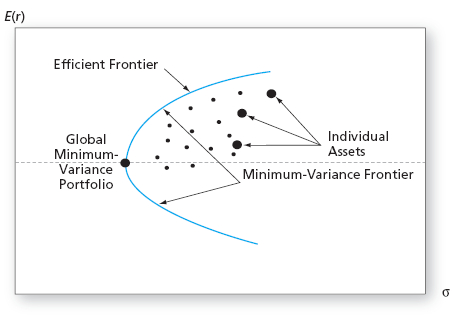
\includegraphics[width=6in]{pg211_1.jpg}


\subsection{Risky Minimum-Variance Frontier}
\label{multiAssetOpt:id4}
The frontier generated by multiple risky assets is known as the risky
minimum-variance (MV) frontier.
\begin{itemize}
\item {} 
The lower portion of the frontier is inefficient since a higher mean
portfolio exists with the same volatility on the upper portion of
the frontier.

\end{itemize}
\begin{itemize}
\item {} 
The efficient MV frontier is generated by allowing investment in a
risk-free asset and finding the CAL which is tangent to the risky
efficient MV frontier.

\end{itemize}


\subsection{Efficient Minimum-Variance Frontier}
\label{multiAssetOpt:efficient-minimum-variance-frontier}
$\qquad$

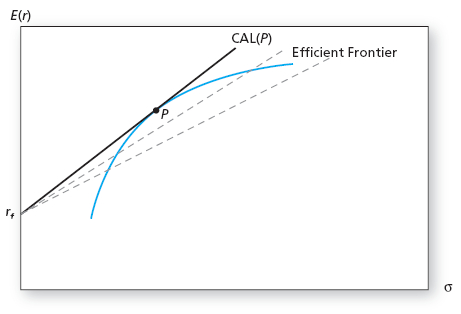
\includegraphics[width=6in]{pg212_2.jpg}


\subsection{Optimization: Efficient MV Frontier}
\label{multiAssetOpt:optimization-efficient-mv-frontier}
To determine the tangency portfolio, the investor solves the same
problem as before
\begin{gather}
\begin{split}\max_{\mu_p, \sigma_p} SR_p = \frac{\mu_p - r_f}{\sigma_p}\end{split}\notag
\end{gather}
subject to
\begin{gather}
\begin{split}\mu_p = \sum_{i=1}^N \omega_i \mu_i\end{split}\notag
\end{gather}\begin{gather}
\begin{split}\sigma_p = \sqrt{\sum_{i=1}^N \omega^2_i \sigma^2_i + 2
\sum_{i=1}^{N-1} \sum_{j=i+1}^N \omega_i \omega_j \sigma_{ij}}.\end{split}\notag
\end{gather}

\subsection{Optimization: Investor Choice}
\label{multiAssetOpt:optimization-investor-choice}
So far we have specified two optimization problems:
\begin{enumerate}
\item {} 
To determine the risky minimum-variance frontier by minimizing
variance subject to a particular expected return.

\end{enumerate}
\begin{enumerate}
\setcounter{enumi}{1}
\item {} 
To determine the tangency portfolio, by maximizing the Sharpe
Ratio subject to constraints on the mean and standard
deviation.

\end{enumerate}

Neither of these made use of preferences.  A final optimization
problem would be the same as before:
\begin{enumerate}
\setcounter{enumi}{2}
\item {} 
Maximize utility, $U(\mu_p, \sigma_p)$, subject to investing
in the tangency portfolio and a risk-free asset.

\end{enumerate}


\subsection{Estimation}
\label{multiAssetOpt:estimation}
In practice we must estimate $\mu_i$, $\sigma^2_i$ and
$\sigma_{ij}$ for $i=1,\ldots,N$ and $j=i+1,\ldots,N$.
\begin{itemize}
\item {} 
A total of $N$ estimates of means.

\end{itemize}
\begin{itemize}
\item {} 
How many variances and covariances must we estimate?

\end{itemize}
\begin{itemize}
\item {} 
A total of $N$ elements on the diagonal (variances).

\end{itemize}
\begin{itemize}
\item {} 
All of the elements above \emph{or} below the diagonal (\emph{not both}
because of symmetry).

\end{itemize}


\subsection{Estimation}
\label{multiAssetOpt:id5}\begin{itemize}
\item {} 
The resulting number of variance and covariance estimates is

\end{itemize}
\begin{gather}
\begin{split}N + (N-1) + (N-2) + \ldots + 2 + 1 & = \sum_{i=1}^N i =
\frac{N(N+1)}{2}.\end{split}\notag
\end{gather}

\subsection{Estimation}
\label{multiAssetOpt:id6}
The total number of estimates is
\begin{gather}
\begin{split}N + \frac{N(N+1)}{2} & = \frac{N(N+3)}{2}.\end{split}\notag
\end{gather}\begin{itemize}
\item {} 
As an example, a portfolio of 50 stocks requires $\frac{50
\times 53}{2} = 1325$ estimates.

\end{itemize}
\begin{itemize}
\item {} 
The models of subsequent lectures will reduce this estimation
burden.

\end{itemize}


\subsection{Portfolio Optimization Recipe}
\label{multiAssetOpt:portfolio-optimization-recipe}
For an arbitrary number, $N$, of risky assets:
\begin{enumerate}
\item {} 
Specify (estimate) the return characteristics of all securities
(means, variances and covariances).

\end{enumerate}
\begin{enumerate}
\setcounter{enumi}{1}
\item {} 
Establish the optimal risky portfolio.

\end{enumerate}
\begin{quote}
\begin{itemize}
\item {} 
Calculate the weights for the tangency portfolio.

\end{itemize}
\begin{itemize}
\item {} 
Compute mean and std. deviation of the tangency portfolio.

\end{itemize}
\end{quote}


\subsection{Portfolio Optimization Recipe}
\label{multiAssetOpt:id7}\begin{enumerate}
\setcounter{enumi}{2}
\item {} 
Allocate funds between the optimal risky portfolio and the
risk-free asset.

\end{enumerate}
\begin{quote}
\begin{itemize}
\item {} 
Calculate the fraction of the complete portfolio allocated to the
tangency portfolio and to the risk-free asset.

\end{itemize}
\begin{itemize}
\item {} 
Calculate the share of the complete portfolio invested in each
asset of the tangency portfolio.

\end{itemize}
\end{quote}


\subsection{Separation Property}
\label{multiAssetOpt:separation-property}
All investors hold some combination of the same two assets: the
risk-free asset and the tangency portfolio.
\begin{itemize}
\item {} 
The optimal risky (tangency portfolio) is the same for all
investors, regardless of preferences.

\end{itemize}
\begin{itemize}
\item {} 
The tangency portfolio is simply determined by estimation and a
mathematical formula.

\end{itemize}
\begin{itemize}
\item {} 
Individual preferences determine the exact proportions of wealth
each investor will allocate to the two assets.

\end{itemize}
\begin{itemize}
\item {} 
This is known as \emph{The Separation Property} (or \emph{Two Fund
Separation}).

\end{itemize}


\subsection{Separation Property}
\label{multiAssetOpt:id8}
The separation property implies that portfolio choice can be separated
into two independent steps:
\begin{itemize}
\item {} 
Determining the optimal risky portfolio (preference independent).

\end{itemize}
\begin{itemize}
\item {} 
Deciding what proportion of wealth to invest in the risk-free asset
and the tangency portfolio (preference dependent).

\end{itemize}


\subsection{Separation Property}
\label{multiAssetOpt:id9}
The separation property will not hold if
\begin{itemize}
\item {} 
Individuals produce different estimates of asset return
characteristics (since differing estimates will result in different
tangency portfolios).

\end{itemize}
\begin{itemize}
\item {} 
Individuals face different constraints (short-sale, tax, etc.).

\end{itemize}


\subsection{The Power of Diversification}
\label{multiAssetOpt:the-power-of-diversification}
Let's formalize the benefits of diversification.  The variance of a
portfolio of $N$ risky assets is
\begin{gather}
\begin{split}\sigma^2_p & = \sum_{i=1}^N \sum_{j=1}^N \omega_i \omega_j
\sigma_{ij} = \sum_{i=1}^N \omega^2_i \sigma^2_i + 2
\sum_{i=1}^{N-1} \sum_{j=i+1}^N \omega_i \omega_j \sigma_{ij}.\end{split}\notag
\end{gather}
In the case of an equally weighted portfolio,
\begin{gather}
\begin{split}\sigma^2_p & = \frac{1}{N^2} \sum_{i=1}^N \sigma^2_i
+ \frac{2}{N^2} \sum_{i=1}^{N-1} \sum_{j=i+1}^N \sigma_{ij} \\
& = \frac{1}{N} \overline{Var} + \frac{N-1}{N}
\overline{Cov}.\end{split}\notag
\end{gather}

\subsection{The Power of Diversification}
\label{multiAssetOpt:id10}
Where
\begin{gather}
\begin{split}\overline{Var} & = \frac{1}{N} \sum_{i=1}^N \sigma^2_i\end{split}\notag
\end{gather}
and
\begin{gather}
\begin{split}\overline{Cov} & = \frac{2}{N(N-1)} \sum_{i=1}^{N-1}
\sum_{j=i+1}^N \sigma_{ij}.\end{split}\notag
\end{gather}
These are the average variance and covariance.


\subsection{The Power of Diversification}
\label{multiAssetOpt:id11}
The limit of portfolio variance is
\begin{gather}
\begin{split}\lim_{N \to \infty} \sigma^2_p & = \lim_{N \to \infty} \frac{1}{N}
\overline{Var} + \lim_{N \to \infty} \frac{N-1}{N}
\overline{Cov} = \overline{Cov}.\end{split}\notag
\end{gather}\begin{itemize}
\item {} 
If the assets in the portfolio are uncorrelated or not correlated
\emph{on average} ($\overline{Cov} = 0$), there is no limit to
diversification: $\sigma^2_p = 0$.

\end{itemize}
\begin{itemize}
\item {} 
If there are systemic sources of risk that affect all assets
($\overline{Cov} > 0$) there will be a lower bound on ability
to diversify: $\sigma^2_p > 0$.

\end{itemize}


\chapter{Index Models}
\label{indexModels::doc}\label{indexModels:index-models}

\section{Motivation}
\label{indexModels:motivation}
Recall that for portfolio optimization with $N$ assets we must
estimate all means, variances and covariances:
\begin{gather}
\begin{split}\# \,\, \text{of estimates} & = \frac{N(N+3)}{2}.\end{split}\notag
\end{gather}
Suppose you have a dataset consisting of 5 years of monthly returns
for each asset (i.e. 60 observations per asset):

\begin{tabulary}{\linewidth}{|L|L|L|L|L|}
\hline
\textsf{\relax 
$N$
} & \textsf{\relax 
50
} & \textsf{\relax 
100
} & \textsf{\relax 
1000
} & \textsf{\relax 
3000
}\\
\hline
\# Estimates
 & 
1325
 & 
5150
 & 
501,500
 & 
4,504,500
\\

Data
 & 
3000
 & 
6000
 & 
60,000
 & 
180,000
\\
\hline\end{tabulary}


Note: it is impossible to estimate $P$ parameters with $N$
data observations if $N < P$.


\section{Motivation}
\label{indexModels:id1}
The return to an asset can \emph{always} be decomposed into two parts:
\begin{gather}
\begin{split}r_i & = E[r_i] + \epsilon_i = \mu_i + \epsilon_i,\end{split}\notag
\end{gather}
where $\epsilon_i$ has zero mean ($\mu_{\epsilon_i} = 0$)
and standard deviation $\sigma_{\epsilon_i}$.
\begin{itemize}
\item {} 
The first term of the equation above is the expected return.

\end{itemize}
\begin{itemize}
\item {} 
The second term is the unexpected, or unanticipated return (also
referred to as a shock).

\end{itemize}
\begin{itemize}
\item {} 
This decomposition is not dependent on a model or special
assumptions.

\end{itemize}


\section{Single-Factor Model}
\label{indexModels:single-factor-model}
Suppose there is a market factor $m$ that influences the returns
to all firms.
\begin{itemize}
\item {} 
Assume we can further decompose the shock, $\epsilon_i$, into
two parts:

\end{itemize}
\begin{gather}
\begin{split}\epsilon_i = \beta_i m + \varepsilon_i.\end{split}\notag
\end{gather}

\section{Single-Factor Model}
\label{indexModels:id2}
In this case the return can be written as a single-factor model:
\phantomsection\label{indexModels:equation-sfm}\begin{gather}
\begin{split}r_i & = \mu_i + \beta_i m + \varepsilon_i.\end{split}\label{indexModels-sfm}\\\begin{split}\end{split}\notag
\end{gather}\begin{itemize}
\item {} 
$m$ and $\varepsilon_i$ have means $\mu_m = \mu_{\varepsilon_i}
= 0$, standard deviations $\sigma_m$ and
$\sigma_{\varepsilon_i}$, and are uncorrelated ($Cov(m, \varepsilon_i) = 0$).

\end{itemize}
\begin{itemize}
\item {} 
$\epsilon_i$ is still unanticipated since $\mu_{\epsilon_i} = \mu_m + \mu_{\varepsilon_i} = 0$.

\end{itemize}
\begin{itemize}
\item {} 
$\beta_i$ is a measure of the sensitivity of $r_i$ to $m$.

\end{itemize}


\section{Decomposing Risk}
\label{indexModels:decomposing-risk}
We can now compute variances using the model:
\begin{gather}
\begin{split}\sigma^2_i & \equiv Var(r_i) = Var(\mu_i + \beta_i m +
\varepsilon_i) \qquad\end{split}\notag
\end{gather}\begin{gather}
\begin{split}& \qquad = \beta^2_i Var(m) + Var(\varepsilon_i) + 2\beta_iCov(m,\varepsilon_i)\end{split}\notag
\end{gather}\begin{gather}
\begin{split}& = \beta^2_i \sigma^2_m + \sigma^2_{\varepsilon_i}. \qquad \qquad
\qquad \quad \,\end{split}\notag
\end{gather}\begin{itemize}
\item {} 
We made use of $Var(\mu_i) = 0$ and $Cov(m,\varepsilon_i) = 0$.

\end{itemize}
\begin{itemize}
\item {} 
$Var(r_i)$ arises from two separate sources.
\begin{itemize}
\item {} 
$\beta^2_i \sigma^2_m$: risk due to $m$. Since this is common to
all assets, it is the systematic component.

\end{itemize}
\begin{itemize}
\item {} 
$\sigma^2_{\varepsilon_i}$: idiosyncratic component specific to each
asset.

\end{itemize}

\end{itemize}


\section{Decomposing Risk}
\label{indexModels:id3}
We can use the model to compute covariances between assets:
\begin{gather}
\begin{split}Cov(r_i,r_j) & = Cov(\mu_i + \beta_i m + \varepsilon_i, \mu_j + \beta_j m + \varepsilon_j)\end{split}\notag
\end{gather}\begin{gather}
\begin{split}& = \beta_i \beta_j Cov(m,m) \qquad \quad\end{split}\notag
\end{gather}\begin{gather}
\begin{split}& = \beta_i \beta_j \sigma^2_m. \qquad \qquad \quad \enspace\end{split}\notag
\end{gather}\begin{itemize}
\item {} 
$Var(\mu_i) = Var(\mu_j) = Cov(\mu_i,\mu_j) = 0$, since $\mu_i$
and $\mu_j$ are constants.

\end{itemize}
\begin{itemize}
\item {} 
We assumed $Cov(\varepsilon_i, \varepsilon_j) = 0$.

\end{itemize}
\begin{itemize}
\item {} 
Intuitively, unanticipated shocks to different assets shouldn't be
correlated.

\end{itemize}


\section{Using an Index as a Factor}
\label{indexModels:using-an-index-as-a-factor}
So what \emph{is} $m$?
\begin{itemize}
\item {} 
We would like to find a macroeconomic variable correlated with all
assets.

\end{itemize}
\begin{itemize}
\item {} 
It is common to use a market index portfolio, such as the S\&P 500
(we expect the return of a broad index to be correlated with
individual assets).

\end{itemize}


\section{Using an Index as a Factor}
\label{indexModels:id4}
In particular, let's use $m = r_m - \mu_m$, where $r_m$ is
the return to the S\&P 500 ($m$ stands for market).
\begin{itemize}
\item {} 
In this case

\end{itemize}
\begin{gather}
\begin{split}E[m] & = E[r_m - \mu_m] \quad\end{split}\notag
\end{gather}\begin{gather}
\begin{split}& \quad = E[r_m] - \mu_m \,\end{split}\notag
\end{gather}\begin{gather}
\begin{split}& = \mu_m - \mu_m \,\end{split}\notag
\end{gather}\begin{gather}
\begin{split}& = 0. \qquad \enspace\end{split}\notag
\end{gather}\begin{itemize}
\item {} 
So our assumption of $E[m] = 0$ is satisfied.

\end{itemize}


\section{Single-Index Model}
\label{indexModels:single-index-model}
Substituting this factor into the single-factor model of
Equation \eqref{indexModels-sfm}:
\begin{gather}
\begin{split}r_i & = \mu_i + \beta_i (r_m - \mu_m) + \varepsilon_i.\end{split}\notag
\end{gather}
We then manipulate the equation:
\begin{gather}
\begin{split}r_i & = r_f - r_f + \mu_i + \beta_i(r_m - r_f + r_f - \mu_m) +
\varepsilon_i \qquad \quad\end{split}\notag
\end{gather}\begin{gather}
\begin{split}& = r_f + \underbrace{(\mu_i - r_f) - \beta_i (\mu_m -
r_f)}_{\alpha_i} + \beta_i (r_m - r_f) + \varepsilon_i \,\end{split}\notag
\end{gather}\phantomsection\label{indexModels:equation-sim}\begin{gather}
\begin{split}\Rightarrow r_{i,e} = \alpha_i + \beta_i r_{m,i} + \varepsilon_i.\end{split}\label{indexModels-sim}\\\begin{split}\end{split}\notag
\end{gather}

\section{Single-Index Model}
\label{indexModels:id5}
Equation \eqref{indexModels-sim} is the single-index model.
\begin{itemize}
\item {} 
Note: $\alpha_i = rp_i - \beta_i rp_m$.

\end{itemize}


\section{Expected Return-Beta Relationship}
\label{indexModels:expected-return-beta-relationship}
Taking expectations of Equation \eqref{indexModels-sim}, we find
\begin{gather}
\begin{split}rp_i & = \alpha_i + \beta_i rp_m,\end{split}\notag
\end{gather}
since $E[\varepsilon_i] = 0$.
\begin{itemize}
\item {} 
$\beta_i$ is known as the security \emph{Beta} and is a measure of
the sensitivity of asset $i$ to the market index.

\end{itemize}
\begin{itemize}
\item {} 
$\beta_i rp_m$ is the systematic risk premium, since it is the
premium one could expect for taking on systematic risk.

\end{itemize}
\begin{itemize}
\item {} 
$\alpha_i$ is the non-market premium. It is the risk premium
expected above that provided by the market.

\end{itemize}

In equilibrium we expect $\alpha_i = 0$.


\section{Why $\alpha$ Must Be Zero}
\label{indexModels:why-must-be-zero}
Why do we expect $\alpha_i = 0$?
\begin{itemize}
\item {} 
Suppose $\alpha_i > 0$.

\end{itemize}
\begin{itemize}
\item {} 
We expect individuals to buy more of asset $i$, putting more
weight on it in their individual portfolios relative to the market
portfolio.

\end{itemize}
\begin{itemize}
\item {} 
If everyone did this, the market portfolio would put higher weight
on asset $i$.
\begin{itemize}
\item {} 
\emph{Everyone} deviates from the market portfolio by holding more of
asset $i$.

\end{itemize}
\begin{itemize}
\item {} 
But since \emph{everyone} constitutes the market, the market portfolio
shifts by the exact amount that they want to hold asset $i$.

\end{itemize}

\end{itemize}


\section{Single-Index Regression}
\label{indexModels:single-index-regression}
We express the single-index model as a regression:
\begin{gather}
\begin{split}r_{i,e}(t) & = \alpha_i + \beta_i r_{m,e}(t) + \varepsilon_i(t),\end{split}\notag
\end{gather}
where the $t$ denotes that the relationship must hold for all
observations through time.
\begin{itemize}
\item {} 
We estimate the model by collecting historical
observations for $r_m$, $r_i$ and $r_f$ and then
computing the regression  estimates for $\alpha_i$
and $\beta_i$.

\end{itemize}


\section{Security Characteristic Line}
\label{indexModels:security-characteristic-line}
The regression estimates of $\alpha_i$ and $\beta_i$ are denoted by
$\hat{\alpha}_i$ and $\hat{\beta}_i$.
\begin{itemize}
\item {} 
The \emph{fitted values} of the regression are

\end{itemize}
\phantomsection\label{indexModels:equation-scl}\begin{gather}
\begin{split}\hat{r}_{i,e}(t) & = \hat{\alpha}_i + \hat{\beta}_i r_{m,e}(t).\end{split}\label{indexModels-scl}\\\begin{split}\end{split}\notag
\end{gather}\begin{itemize}
\item {} 
$\hat{r}_{i,e}(t)$ are the values of the regression line.

\end{itemize}
\begin{itemize}
\item {} 
They are the values we \emph{expect} $r_{i,e}$ to take for given
values of $r_{m,e}$.

\end{itemize}


\section{Security Characteristic Line}
\label{indexModels:id6}\begin{itemize}
\item {} 
Residuals are not included since they are \emph{unexpected} (deviations
from the line).

\end{itemize}
\begin{itemize}
\item {} 
Equation \eqref{indexModels-scl} is known as the \emph{Security Characteristic Line} or
SCL.

\end{itemize}


\section{Advantages of the Model}
\label{indexModels:advantages-of-the-model}
Suppose we want to use the Index Model to produce the estimates
required for portfolio optimization.
\begin{itemize}
\item {} 
Assume there are $N$ assets in the portfolio.

\end{itemize}
\begin{itemize}
\item {} 
From the model,

\end{itemize}
\begin{gather}
\begin{split}\mu_{i,e} & = \alpha_i + \beta_i \mu_{m,e}\end{split}\notag
\end{gather}\begin{gather}
\begin{split}\sigma^2_i & = \beta^2_i \sigma^2_m + \sigma^2_{\varepsilon_i}\end{split}\notag
\end{gather}
and
\begin{gather}
\begin{split}\sigma_{ij} & = \beta_i \beta_j \sigma^2_m.\end{split}\notag
\end{gather}

\section{Advantages of the Model}
\label{indexModels:id7}
Let's count the number of parameters we must estimate.
\begin{itemize}
\item {} 
$N$ estimates of $\alpha_i$.

\end{itemize}
\begin{itemize}
\item {} 
$N$ estimates of $\beta_i$.

\end{itemize}
\begin{itemize}
\item {} 
$N$ estimates of $\sigma^2_{\varepsilon_i}$.

\end{itemize}
\begin{itemize}
\item {} 
One estimate of $\mu_m$.

\end{itemize}
\begin{itemize}
\item {} 
One estimate of $\sigma_m$.

\end{itemize}


\section{Advantages of the Model}
\label{indexModels:id8}
That's a total of $3N+2$ estimates.
\begin{itemize}
\item {} 
We'll see this is much better than $\frac{N(N+3)}{2}$
estimates without the model.

\end{itemize}


\section{Advantages of the Model}
\label{indexModels:id9}
Suppose you have a dataset consisting of 5 years of monthly returns
for each asset (i.e. 60 observations per asset):

\begin{tabulary}{\linewidth}{|L|L|L|L|L|}
\hline
\textsf{\relax 
$N$
} & \textsf{\relax 
50
} & \textsf{\relax 
100
} & \textsf{\relax 
1000
} & \textsf{\relax 
3000
}\\
\hline
\# Estimates No Model
 & 
1325
 & 
5150
 & 
501,500
 & 
4,504,500
\\

\# Estimates Index Model
 & 
152
 & 
302
 & 
3002
 & 
9002
\\

Data
 & 
3000
 & 
6000
 & 
60,000
 & 
180,000
\\
\hline\end{tabulary}


Clearly estimation is much more reasonable with the single-index model
for large $N$.


\section{Cost of the Model}
\label{indexModels:cost-of-the-model}
The index model restricts the relationship among the asset variances
and covariances to be of a specific form.
\begin{itemize}
\item {} 
It is precisely this imposed structure that relieves us of the
estimation burden.

\end{itemize}
\begin{itemize}
\item {} 
However, it oversimplifies the true nature of the world.

\end{itemize}
\begin{itemize}
\item {} 
For example, it dichotomizes security risk into two components:
market and asset specific.

\end{itemize}
\begin{itemize}
\item {} 
But neglects to account for industry specific risk, etc.

\end{itemize}
\begin{itemize}
\item {} 
In this sense, the model may fail to capture important aspects of
market.

\end{itemize}


\section{Index Model Portfolios}
\label{indexModels:index-model-portfolios}
Suppose you hold a portfolio of $N$ assets with
weights $\omega_i$, $i=1,\ldots,N$.
\begin{itemize}
\item {} 
Then

\end{itemize}
\begin{gather}
\begin{split}r_{p,e} & = \sum_{i=1}^N \omega_i r_{i,e} = \sum_{i=1}^N \omega_i
(\alpha_i + \beta_i r_{m,e} + \varepsilon_i) \qquad\end{split}\notag
\end{gather}\begin{gather}
\begin{split}& \,= \underbrace{\sum_{i=1}^N \omega_i \alpha_i}_{\alpha_p} +
\underbrace{\left(\sum_{i=1}^N \omega_i \beta_i \right)}_{\beta_p}
r_{m,e} + \underbrace{\sum_{i=1}^N \omega_i \varepsilon_i}_{\varepsilon_p}\end{split}\notag
\end{gather}\begin{gather}
\begin{split}& = \alpha_p + \beta_p r_{m,e} + \varepsilon_p. \qquad \qquad
\qquad \quad\end{split}\notag
\end{gather}

\section{Index Model Portfolio Coefficients}
\label{indexModels:index-model-portfolio-coefficients}
The mathematics highlight some very nice results.
\begin{itemize}
\item {} 
$\alpha_p$: The non-market return of the portfolio is a
weighted average of the non-market returns of individual assets.

\end{itemize}
\begin{itemize}
\item {} 
$\beta_p$: The sensitivity of the portfolio to the market
excess return is a weighted average of the sensitivities of
individual assets.

\end{itemize}
\begin{itemize}
\item {} 
$\varepsilon_p$: The portfolio shock is a weighted average of
individual shocks.

\end{itemize}


\section{Index Model Portfolio Risk}
\label{indexModels:index-model-portfolio-risk}
Since the portfolio is described by a single index model, its risk can
be decomposed as
\begin{gather}
\begin{split}\sigma^2_p & = \beta^2_p \sigma^2_m + \sigma^2_{\varepsilon_p}.\end{split}\notag
\end{gather}
Note that,
\begin{gather}
\begin{split}\beta^2_p & = \left(\sum_{i=1}^N \omega_i \beta_i\right)^2\end{split}\notag
\end{gather}
\emph{not}
\begin{gather}
\begin{split}\beta^2_p & = \sum_{i=1}^N \omega^2_i \beta^2_i.\end{split}\notag
\end{gather}

\section{Index Model Portfolio Risk}
\label{indexModels:id10}
The variance of $\varepsilon_p$ can be written as
\phantomsection\label{indexModels:equation-simsigeps1}\begin{gather}
\begin{split}\sigma^2_{\varepsilon_p} & \equiv Var(\varepsilon_p) =
        Var\left(\sum_{i=1}^N \omega_i \varepsilon_i \right)\end{split}\label{indexModels-simsigeps1}\\\begin{split}\end{split}\notag
\end{gather}\phantomsection\label{indexModels:equation-simsigeps2}\begin{gather}
\begin{split}& = \sum_{i=1}^N \omega^2_i Var(\varepsilon_i) \qquad \quad \enspace\end{split}\label{indexModels-simsigeps2}\\\begin{split}\end{split}\notag
\end{gather}\phantomsection\label{indexModels:equation-simsigeps3}\begin{gather}
\begin{split}& = \sum_{i=1}^N \omega^2_i \sigma^2_{\varepsilon_i} \qquad
        \qquad \quad\end{split}\label{indexModels-simsigeps3}\\\begin{split}\end{split}\notag
\end{gather}
Equation \eqref{indexModels-simsigeps2} follows from Equation \eqref{indexModels-simsigeps1}
because we assume that $Cov(\varepsilon_i, \varepsilon_j) = 0$ for $i
\neq j$.


\section{Index Model Diversification}
\label{indexModels:index-model-diversification}
In the special case of an equally-weighted portfolio
\begin{gather}
\begin{split}\sigma^2_{\varepsilon_p} = \frac{1}{N^2} \sum_{i=1}^N \sigma^2_{\varepsilon_i} = \frac{1}{N} \overline{\sigma^2_{\varepsilon_p}},\end{split}\notag
\end{gather}
where
\begin{gather}
\begin{split}\overline{\sigma^2_{\varepsilon_p}} = \frac{1}{N} \sum_{i=1}^N \sigma^2_{\varepsilon_i}.\end{split}\notag
\end{gather}
Clearly,
\begin{gather}
\begin{split}\lim_{N \to \infty} \overline{\sigma^2_{\varepsilon_p}} & = 0.\end{split}\notag
\end{gather}

\section{Index Model Diversification}
\label{indexModels:id11}
Recall
\begin{gather}
\begin{split}\sigma^2_p & = \beta^2_p \sigma^2_m + \sigma^2_{\varepsilon_p}.\end{split}\notag
\end{gather}
Thus,
\begin{gather}
\begin{split}\lim_{N \to \infty} \sigma^2_p & = \lim_{N \to \infty} \beta^2_p
\sigma^2_m + \lim_{N \to \infty} \sigma^2_{\varepsilon_p}\end{split}\notag
\end{gather}\begin{gather}
\begin{split}& = \beta^2_p \sigma^2_m.\end{split}\notag
\end{gather}

\section{Index Model Diversification}
\label{indexModels:id12}
$\qquad$

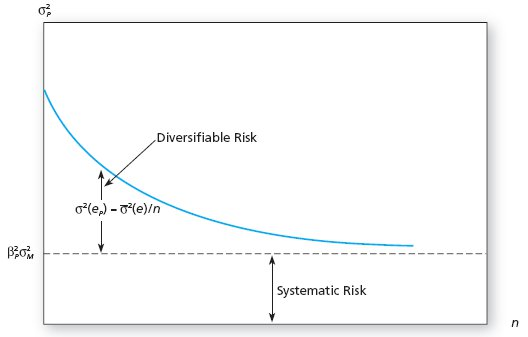
\includegraphics[width=6in]{pg254_1.jpg}


\section{Index Model Example}
\label{indexModels:index-model-example}
Let's estimate an index model.
\begin{itemize}
\item {} 
Use SPY (S\&P 500 SPDR) as a surrogate for market returns.

\end{itemize}
\begin{itemize}
\item {} 
Estimate the model for SWY (Safeway).

\end{itemize}
\begin{itemize}
\item {} 
Download 5 years of monthly data from Yahoo Finance, between 1 Jan
2007 and 31 Dec 2012.

\end{itemize}
\begin{itemize}
\item {} 
Use adjusted closing prices to compute returns.

\end{itemize}
\begin{itemize}
\item {} 
Estimate the regression.

\end{itemize}


\section{Index Model Example}
\label{indexModels:id13}
$\qquad$

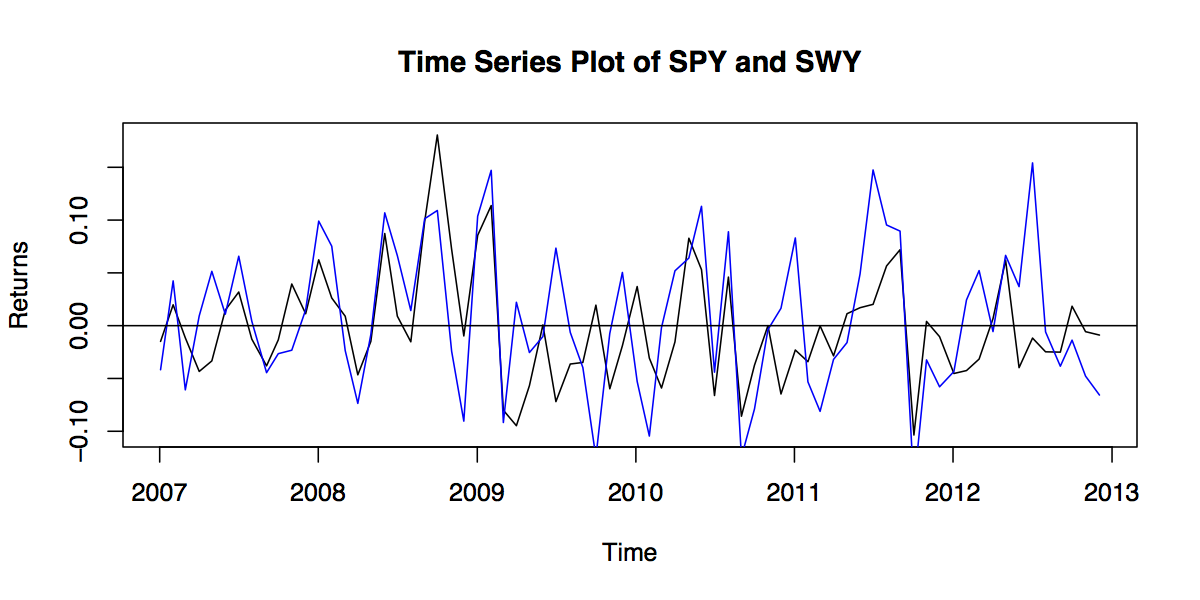
\includegraphics[width=6in]{spy-swy-tsplot.png}


\section{Index Model Example}
\label{indexModels:id14}
\begin{tabulary}{\linewidth}{|L|L|L|L|}
\hline
\textsf{\relax 
Parameter
} & \textsf{\relax 
Estimate
} & \textsf{\relax 
Standard Error
} & \textsf{\relax 
P-Value
}\\
\hline
$\alpha$
 & 
0.003903
 & 
0.007387
 & 
0.599
\\

$\beta$
 & 
0.7620
 & 
0.1319
 & 
1.92e-07
\\
\hline\end{tabulary}


The Adjusted $R^2$ is 0.3133.


\section{Index Model Example}
\label{indexModels:id15}
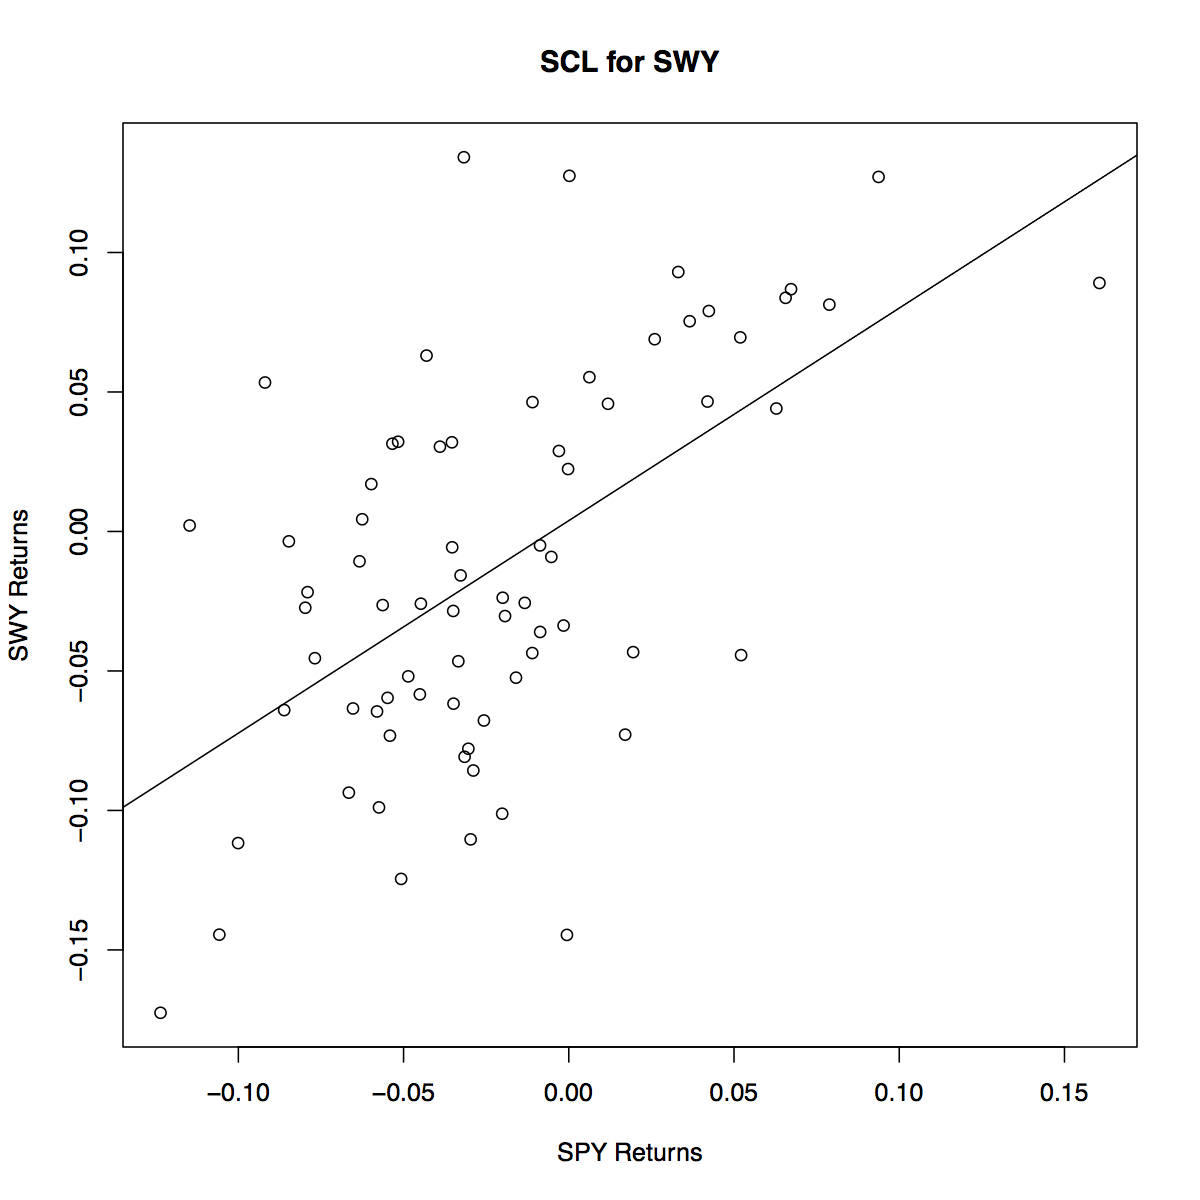
\includegraphics[width=6in]{spy-swy-reg.png}


\chapter{Bonds}
\label{bonds::doc}\label{bonds:bonds}
Contents:


\section{Bond Prices and Yields}
\label{bondPrices:bond-prices-and-yields}\label{bondPrices::doc}

\subsection{Bond Basics}
\label{bondPrices:bond-basics}
A bond is a financial asset used to facilitate borrowing and lending.
\begin{itemize}
\item {} 
A borrower has an obligation to make pre-specified payments to the
lender on specific dates.

\end{itemize}
\begin{itemize}
\item {} 
Bonds are generally referred to as fixed-income securities.
\begin{itemize}
\item {} 
Historically, their payments have been  fixed.

\end{itemize}
\begin{itemize}
\item {} 
In general, they can have variable payments, but those payments
are determined by a formula.

\end{itemize}

\end{itemize}
\begin{itemize}
\item {} 
At the end of the bond's maturity, the borrower pays the \emph{face
value}, or \emph{par value} of the bond to the lender.

\end{itemize}


\subsection{Coupons}
\label{bondPrices:coupons}
Typical coupon bonds require the borrower to make semiannual coupon
payments to the lender.
\begin{itemize}
\item {} 
The coupon rate is the total annual amount paid in coupons divided
by the face value.

\end{itemize}
\begin{itemize}
\item {} 
Zero-coupon bonds pay no coupons - they simply pay the face value at
maturity.

\end{itemize}
\begin{itemize}
\item {} 
The only way for such assets to be marketable is for their sale
value to be below the face value.

\end{itemize}


\subsection{Bond Example}
\label{bondPrices:bond-example}
Suppose a semiannual coupon bond has a face value of \$1000 and a
coupon rate of 8\%.
\begin{itemize}
\item {} 
The total amount of coupons paid annually is

\end{itemize}
\begin{gather}
\begin{split}0.08*\$1000 = \$80.\end{split}\notag\\\begin{split}\end{split}\notag
\end{gather}\begin{itemize}
\item {} 
Since coupons are paid semiannually, this amount is divided by two.

\end{itemize}
\begin{itemize}
\item {} 
So a \$40 coupon is paid every six months and \$1000 is paid at
maturity.

\end{itemize}


\subsection{Government Bonds}
\label{bondPrices:government-bonds}
U.S. Government debt assets fall into three categories.
\begin{itemize}
\item {} 
Treasury bills (T-bills). These pay no coupons and mature in one
year or less from the time of issue.

\end{itemize}
\begin{itemize}
\item {} 
Treasury notes. These typically pay semiannual coupons and mature in
2 to 10 years from the time of issue (typical maturities are 2, 5
and 10 years).

\end{itemize}
\begin{itemize}
\item {} 
Treasury bonds. These typically pay semiannual coupons and mature
between 10 to 30 years from the time of issue.

\end{itemize}


\subsection{Government Bonds}
\label{bondPrices:id1}
$\qquad$

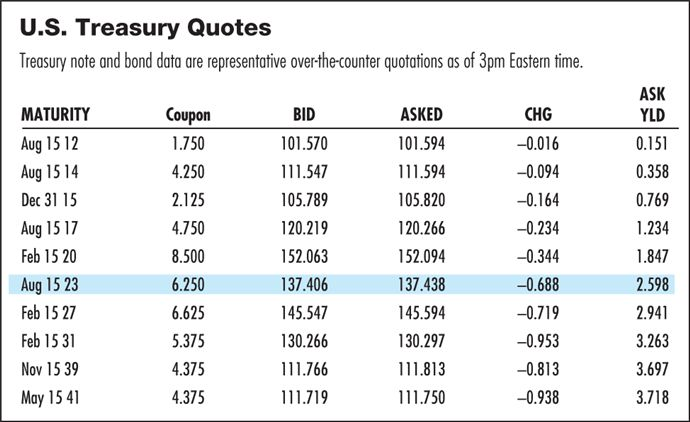
\includegraphics[width=6in]{bod34698_1001_lg.jpg}


\subsection{Corporate Bonds}
\label{bondPrices:corporate-bonds}
U.S. corporations also issue bonds in order to borrow money. These
debt instruments are generally quite similar to their government
counterparts.
\begin{gather}
\begin{split}\qquad\end{split}\notag\\\begin{split}\end{split}\notag
\end{gather}
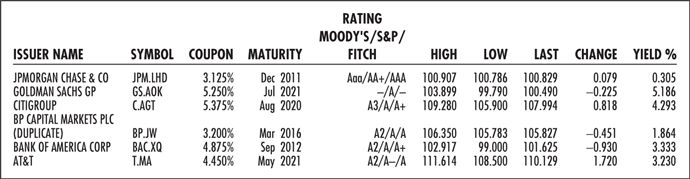
\includegraphics[width=6in]{bod34698_1002_lg.jpg}


\subsection{Treasury Inflation Protected Securities}
\label{bondPrices:treasury-inflation-protected-securities}
Typical bonds offer nominal returns that don't account for inflation.
\begin{itemize}
\item {} 
TIPS are bonds whose face values (and hence their coupons) are
indexed to the general level of prices.

\end{itemize}
\begin{itemize}
\item {} 
If inflation is equal to 2\% over the course of a year, the face
value of the bond will also rise by 2\%.

\end{itemize}
\begin{itemize}
\item {} 
The result is a bond with no inflation risk and which should offer a
rate of return that is equal to the real, risk-free rate.

\end{itemize}


\subsection{TIPS Example}
\label{bondPrices:tips-example}
Consider the following bond.
\begin{itemize}
\item {} 
Face value = \$1000.

\end{itemize}
\begin{itemize}
\item {} 
Coupon rate = 4\%.

\end{itemize}
\begin{itemize}
\item {} 
Annual coupon, with three years to maturity.

\end{itemize}
\begin{itemize}
\item {} 
Inflation will be 2\%, 3\% and 1\% for the next three years.

\end{itemize}


\subsection{TIPS Example}
\label{bondPrices:id2}
$\qquad$

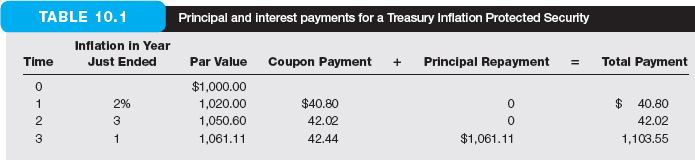
\includegraphics[width=6in]{table10_1_lg.jpg}


\subsection{TIPS Example}
\label{bondPrices:id3}
We can compute the nominal and real rates of return.
\begin{gather}
\begin{split}r_{nom} & = \frac{\text{Interest} + \text{Price
Appreciation}}{\text{Initial Price}}\end{split}\notag
\end{gather}\begin{gather}
\begin{split}& = \frac{40.80 + 20}{1000} \qquad \qquad \enspace \;\end{split}\notag
\end{gather}\begin{gather}
\begin{split}& = 0.0608 \qquad \qquad \quad \quad \; \,\end{split}\notag
\end{gather}

\subsection{TIPS Example}
\label{bondPrices:id4}\begin{gather}
\begin{split}r_{real} & = \frac{1+\text{Nominal Return}}{1+\text{Inflation}} - 1\end{split}\notag
\end{gather}\begin{gather}
\begin{split}& = \frac{1.0608}{1.02} - 1 \qquad \quad \:\end{split}\notag
\end{gather}\begin{gather}
\begin{split}& = 0.04. \qquad \qquad \quad \enspace\end{split}\notag
\end{gather}

\subsection{TIPS Example}
\label{bondPrices:id5}
The real rate of return is simply equal to the coupon rate.
\begin{itemize}
\item {} 
Inflation has been eliminated since the bond's face value has
implicitly incorporated it into the value by tying its face value to
increases in prices.

\end{itemize}


\subsection{STRIPS}
\label{bondPrices:strips}
STRIPS stands for ``Separate Trading of Registered Interest and
Principle of Securities''.
\begin{itemize}
\item {} 
It is a U.S. Treasury program which identifies bond payments as a
separate securities.

\end{itemize}
\begin{itemize}
\item {} 
A coupon paying bond can be ``stripped'' into multiple assets - each
coupon and the face value being marketed as individual zero-coupon
bonds.
\begin{itemize}
\item {} 
A 10 year, semiannual bond is comprised of 20 coupon payments and
a final payment of the face value.

\end{itemize}
\begin{itemize}
\item {} 
It could be stripped into 21 separate, zero-coupon assets with
varying maturities.

\end{itemize}

\end{itemize}


\subsection{Discounting Cash Flows}
\label{bondPrices:discounting-cash-flows}
A bond's value should be equal to the net present value of its cash flows.
\begin{itemize}
\item {} 
Each payment should be discounted by the product of interest rates
over the period of interest.

\end{itemize}
\begin{itemize}
\item {} 
For a coupon payment in four years

\end{itemize}
\begin{gather}
\begin{split}PV & = \frac{C}{(1+r_1)(1+r_2)(1+r_3)(1+r_4)}.\end{split}\notag
\end{gather}\begin{itemize}
\item {} 
$r_i$ is the interest rate over year $i$.

\end{itemize}


\subsection{Discounting Cash Flows}
\label{bondPrices:id6}
Assuming the interest rate is constant over all periods ($r_i =
r, \forall i$)
\begin{gather}
\begin{split}PV & = \frac{C}{(1+r)^4}.\end{split}\notag
\end{gather}

\subsection{Geometric Series}
\label{bondPrices:geometric-series}
The following mathematical result will be useful for deriving the
value of a bond:
\begin{itemize}
\item {} 
For $|x| < 1$,

\end{itemize}
\begin{gather}
\begin{split}\sum_{i=0}^{\infty} a \, x^i & = \frac{a}{1-x}.\end{split}\notag
\end{gather}

\subsection{Bond Pricing}
\label{bondPrices:bond-pricing}
Let $F$ = Face Value, $C$ = Coupon Payment and $V$ =
Bond Value.
\begin{itemize}
\item {} 
Then,

\end{itemize}
\begin{gather}
\begin{split}V & = \frac{C}{1+r} + \frac{C}{(1+r)^2} + \frac{C}{(1+r)^3} +
\ldots + \frac{C}{(1+r)^T} + \frac{F}{(1+r)^T}\end{split}\notag
\end{gather}\begin{gather}
\begin{split}& = \sum_{i=1}^T \frac{C}{(1+r)^i} + \frac{F}{(1+r)^T} \qquad
\qquad \qquad \qquad \qquad \quad \enspace \,\end{split}\notag
\end{gather}\begin{gather}
\begin{split}& = \sum_{i=1}^{\infty} \frac{C}{(1+r)^i} - \sum_{i=T+1}^{\infty}
\frac{C}{(1+r)^i} + \frac{F}{(1+r)^T} \qquad \qquad \quad \enspace\end{split}\notag
\end{gather}

\subsection{Bond Pricing}
\label{bondPrices:id7}\begin{gather}
\begin{split}& = \sum_{i=1}^{\infty} \frac{C}{(1+r)^i} - \frac{1}{(1+r)^T}
\sum_{i=1}^{\infty} \frac{C}{(1+r)^i} + \frac{F}{(1+r)^T} \qquad\end{split}\notag
\end{gather}\begin{gather}
\begin{split}\hspace{0.25in} & = \left(\sum_{i=1}^{\infty}
\frac{C}{(1+r)^i}\right) \left(1 - \frac{1}{(1+r)^T}\right) +
\frac{F}{(1+r)^T} \qquad \qquad \,\end{split}\notag
\end{gather}\begin{gather}
\begin{split}& = \frac{C}{1+r} \left(\sum_{i=0}^{\infty}
\frac{1}{(1+r)^i}\right) \left(1 - \frac{1}{(1+r)^T}\right) +
\frac{F}{(1+r)^T} \, \,\end{split}\notag
\end{gather}\begin{gather}
\begin{split}& = \frac{C}{1+r} \left(\frac{1}{1-\frac{1}{1+r}}\right) \left(1 -
\frac{1}{(1+r)^T}\right) + \frac{F}{(1+r)^T} \qquad \,\end{split}\notag
\end{gather}

\subsection{Bond Pricing}
\label{bondPrices:id8}\begin{gather}
\begin{split}& = \frac{C}{1+r} \left(\frac{1}{\frac{1+r-1}{1+r}}\right)
\left(1 - \frac{1}{(1+r)^T}\right) + \frac{F}{(1+r)^T} \; \;\end{split}\notag
\end{gather}\begin{gather}
\begin{split}\hspace{0.25in} & = \frac{C}{1+r} \frac{1+r}{r} \left(1 -
\frac{1}{(1+r)^T}\right) + \frac{F}{(1+r)^T} \qquad \;\end{split}\notag
\end{gather}\begin{gather}
\begin{split}& = \frac{C}{r} \left(1 - \frac{1}{(1+r)^T}\right) +
\frac{F}{(1+r)^T}. \qquad \qquad\end{split}\notag
\end{gather}
We made use of the geometric series result,
recognizing $0 < x = \frac{1}{1+r} < 1$.


\subsection{Bond Value Formula}
\label{bondPrices:bond-value-formula}
The bond price formula can be decomposed as
\phantomsection\label{bondPrices:equation-bondprice}\begin{gather}
\begin{split}V & = \frac{C}{r} \left(1 - \frac{1}{(1+r)^T}\right) +
\frac{F}{(1+r)^T} \qquad \qquad \quad \enspace\end{split}\label{bondPrices-bondprice}\\\begin{split}\end{split}\notag
\end{gather}\begin{gather}
\begin{split}& = C \times \underbrace{\left[\frac{1}{r} \left(1 -
\frac{1}{(1+r)^T}\right)\right]}_{\text{Annuity factor}(r,T)} + F
\times \underbrace{\left[\frac{1}{(1+r)^T}\right]}_{\text{PV
factor}(r,T)}.\end{split}\notag
\end{gather}\begin{itemize}
\item {} 
$\text{Annuity factor}(r,T)$ is the present value of a \$1
annuity that lasts for $T$ periods with interest rate
$r$.

\end{itemize}
\begin{itemize}
\item {} 
$\text{PV factor}(r,T)$ is the present value of \$1 paid in
$T$ periods.

\end{itemize}


\subsection{Value vs. Price}
\label{bondPrices:value-vs-price}
So far we have only computed the \emph{present value} of the bond.
\begin{itemize}
\item {} 
What is its price?

\end{itemize}
\begin{itemize}
\item {} 
The bond price should be equal to the present value of payments.

\end{itemize}
\begin{itemize}
\item {} 
If the price was lower, you could buy the bond for $P < V$ and
receive the promised cash flow: your net gain would be $V -
P$.

\end{itemize}
\begin{itemize}
\item {} 
If the price was higher, you could short the bond for $P > V$
and pay the promised cash flow: your net gain would be $P -
V$.

\end{itemize}


\subsection{Bond Pricing Example}
\label{bondPrices:bond-pricing-example}
Consider a bond with the following characteristics.
\begin{itemize}
\item {} 
$F = \$1000$.

\end{itemize}
\begin{itemize}
\item {} 
30 years to maturity.

\end{itemize}
\begin{itemize}
\item {} 
8\% coupon rate.

\end{itemize}
\begin{itemize}
\item {} 
Semiannual coupons.

\end{itemize}

Suppose the nominal interest rate is constant at 8\% for the next 30
years.  Note that
\begin{itemize}
\item {} 
The coupon payment is \$40 every six months.

\end{itemize}
\begin{itemize}
\item {} 
There are 60, six-month time periods.

\end{itemize}


\subsection{Bond Pricing Example}
\label{bondPrices:id9}
The bond price is
\begin{gather}
\begin{split}P & = \frac{\$40}{0.04}\left(1 - \frac{1}{1.04^{60}}\right) +
\frac{\$1000}{1.04^{60}} = \$1000.\end{split}\notag
\end{gather}\begin{itemize}
\item {} 
If the annual interest rate equals the coupon rate, $P = F$.

\end{itemize}

If $r = 0.10$, then
\begin{gather}
\begin{split}P & = \frac{\$40}{0.05}\left(1 - \frac{1}{1.05^{60}}\right) +
\frac{\$1000}{1.05^{60}} = \$810.71.\end{split}\notag
\end{gather}

\subsection{Prices and Yields}
\label{bondPrices:prices-and-yields}
The return for holding a bond is typically referred to as a \emph{yield}.
\begin{itemize}
\item {} 
A central feature of bonds is that prices and yields are negatively
related.

\end{itemize}
\begin{itemize}
\item {} 
Since a bond promises a fixed payment at maturity, you want to
purchase for a very low price.

\end{itemize}


\subsection{Prices and Yields}
\label{bondPrices:id10}
Think of a zero-coupon bond that costs $P$ and pays $F$ at
maturity.
\begin{itemize}
\item {} 
The yield, $y$, is the value such that $P \times (1+y) = F$:

\end{itemize}
\begin{gather}
\begin{split}y & = \frac{F}{P} - 1.\end{split}\notag
\end{gather}\begin{itemize}
\item {} 
Note that $y$ is a net return (not gross).

\end{itemize}
\begin{itemize}
\item {} 
Since the bond price is in the denominator, $y$ and $P$
have an inverse relationship: higher prices mean lower yields.

\end{itemize}
\begin{itemize}
\item {} 
This relationship holds for coupon bonds as well (as seen in the
bond pricing formula in Equation \eqref{bondPrices-bondprice}).

\end{itemize}


\subsection{Prices and Yields}
\label{bondPrices:id11}
Consider a zero-coupon bond with a face value of \$1000 and one period
until maturity.
\begin{itemize}
\item {} 
If $P = \$990$, the yield is

\end{itemize}
\begin{gather}
\begin{split}y & = \frac{\$1000}{\$990} - 1 = 0.01010.\end{split}\notag
\end{gather}\begin{itemize}
\item {} 
If $P = \$995$, the yield is

\end{itemize}
\begin{gather}
\begin{split}y & = \frac{\$1000}{\$995} - 1 = 0.005025.\end{split}\notag
\end{gather}

\subsection{Coupon Rate and Yield}
\label{bondPrices:coupon-rate-and-yield}
We saw above that if the market interest rate $r$ is equal to
the coupon rate, $P = F$.
\begin{itemize}
\item {} 
Consider two competing investments: put your money in a savings
account that pays $r$ each period, or buy a bond.

\end{itemize}
\begin{itemize}
\item {} 
If the coupon rate is exactly equal to $r$, then the bond
exactly compensates you for market return and does not need to
provide price appreciation.

\end{itemize}


\subsection{Coupon Rate and Yield}
\label{bondPrices:id12}\begin{itemize}
\item {} 
If the coupon rate is less than $r$, the bond does not
compensate you enough - to be competitive, it must sell at a
discount (less than the face value).

\end{itemize}
\begin{itemize}
\item {} 
If the coupon rate is greater than $r$, the bond
overcompensates you - to be competitive, it can sell at a premium
(more than the face value).

\end{itemize}


\subsection{Coupon Rate and Yield}
\label{bondPrices:id13}
Why would a borrower sell a bond at a discount when $r$ is
greater than the coupon rate?
\begin{itemize}
\item {} 
Because nobody would buy the bond unless the price formula holds.

\end{itemize}


\subsection{Coupon Rate and Yield}
\label{bondPrices:id14}
Later, the bond price will fluctuate on the secondary market.
\begin{itemize}
\item {} 
If the market rate rises, investors will sell the bond (because of
its low coupon).
\begin{itemize}
\item {} 
The price will fall until the overall return is commensurate with
the market return.

\end{itemize}

\end{itemize}
\begin{itemize}
\item {} 
If the market rate falls, investors will buy the bond
(because of its high coupon).
\begin{itemize}
\item {} 
The price will rise until the overall return is commensurate with
the market return.

\end{itemize}

\end{itemize}


\subsection{Interest Rate Risk}
\label{bondPrices:interest-rate-risk}
Unfortunately, interest rates don't remain constant.
\begin{itemize}
\item {} 
Suppose you purchase a bond for the face value when the coupon rate
and market interest rates are equal.

\end{itemize}
\begin{itemize}
\item {} 
If the market rate suddenly rises, you will have your money tied up
in an investment paying a rate that is too low (opportunity cost).

\end{itemize}
\begin{itemize}
\item {} 
If you sell the bond on the secondary market, the price will be
lower than the face (your purchase price) because $r$ is
greater than the coupon rate.

\end{itemize}


\subsection{Interest Rate Risk}
\label{bondPrices:id15}
The opposite would be true if the market rate falls.
\begin{itemize}
\item {} 
As a result, bond holders are subject to interest rate fluctuations,
or interest rate risk.

\end{itemize}


\subsection{Maturity Risk}
\label{bondPrices:maturity-risk}
Interest rate risk is exacerbated over longer maturities.
\begin{itemize}
\item {} 
Suppose the market interest rate moves after you purchase two bonds
with 10 and 30 years to maturity.

\end{itemize}
\begin{itemize}
\item {} 
If the market rate rises you will suffer a greater loss on the 30
year bond since your money is tied to it for a longer period.

\end{itemize}
\begin{itemize}
\item {} 
As a result, prices of longer maturity bonds are more sensitive to
interest rate movements.

\end{itemize}


\subsection{Maturity Risk}
\label{bondPrices:id16}
$\qquad$

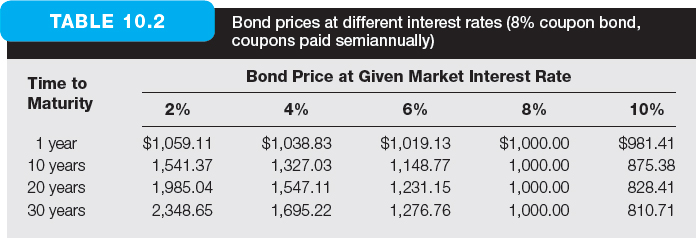
\includegraphics[width=6in]{table10_2_lg.jpg}


\subsection{Bond Prices Over Time}
\label{bondPrices:bond-prices-over-time}
As a bond approaches maturity, its price will approach the face
value.
\begin{itemize}
\item {} 
Fewer payments are subject to interest rate fluctuations.

\end{itemize}
\begin{itemize}
\item {} 
This is true whether the bond sells at a premium or discount.

\end{itemize}


\subsection{Bond Prices Over Time}
\label{bondPrices:id17}
Consider buying a bond the day before maturity.
\begin{quote}
\begin{itemize}
\item {} 
If a coupon is paid at maturity, you only receive a prorated share
of the coupon (one day's worth).

\end{itemize}
\begin{itemize}
\item {} 
Net of the prorated coupon, you should pay only the slightest
discount to face value.

\end{itemize}
\begin{itemize}
\item {} 
The slight discount arises because you can invest your money
overnight and earn a small amount of interest.

\end{itemize}
\end{quote}


\section{The Term Structure of Interest Rates}
\label{termStructure:the-term-structure-of-interest-rates}\label{termStructure::doc}

\subsection{Yield Curve}
\label{termStructure:yield-curve}
Bonds of different maturities often have different yields to maturity.
\begin{itemize}
\item {} 
The relationship between yield and maturity is summarized
graphically in the \emph{yield curve}.

\end{itemize}
\begin{itemize}
\item {} 
Consider several examples below.

\end{itemize}

$\qquad$

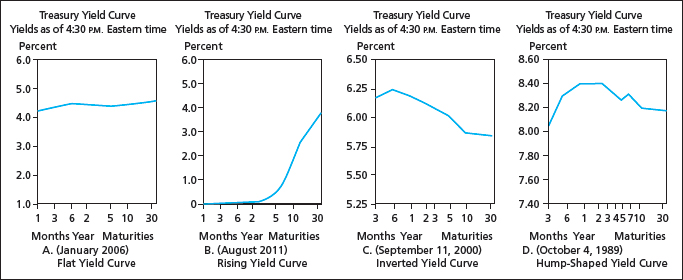
\includegraphics[width=6in]{bod34698_1012_lg.jpg}


\subsection{Yield Curve Slope}
\label{termStructure:yield-curve-slope}
An upward sloping yield curve is evidence that short-term interest
rates are going to rise.
\begin{itemize}
\item {} 
Consider two investment strategies.
\begin{itemize}
\item {} 
Buy and hold a two-year zero-coupon bond, offering 6\% return each
year.

\end{itemize}
\begin{itemize}
\item {} 
Buy a one-year bond today, offering a 5\% return over the coming
year, and roll the investment into another one-year zero-coupon
bond a year from now, offering an interest rate of $r_2$.

\end{itemize}
\begin{itemize}
\item {} 
These investments should be equivalent. Why?

\end{itemize}

\end{itemize}


\subsection{Yield Curve Slope}
\label{termStructure:id1}
Suppose you begin with \$890 to invest (the price of a two-year
zero-coupon bond with 6\% YTM.
\begin{itemize}
\item {} 
Equating the returns to each strategy gives:

\end{itemize}
\begin{gather}
\begin{split}\$890 \times (1.06)^2 & = \$890 \times (1.05) \times (1+r_2)\end{split}\notag
\end{gather}\begin{gather}
\begin{split}\Rightarrow 1 + r_2 & = \frac{1.06^2}{1.05} = 1.0701\end{split}\notag
\end{gather}\begin{gather}
\begin{split}\Rightarrow r_2 & = 0.0701.\end{split}\notag
\end{gather}

\subsection{Two Investment Strategies}
\label{termStructure:two-investment-strategies}
$\qquad$

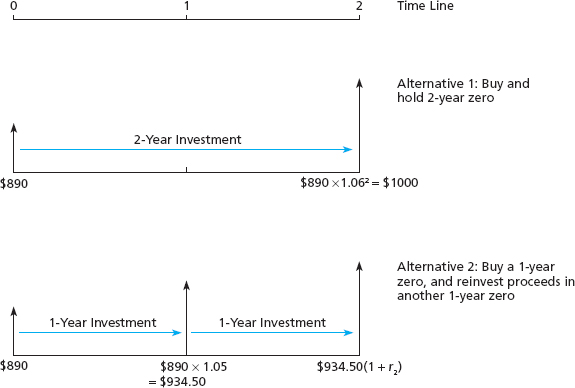
\includegraphics[width=6in]{pg484_1.jpg}


\subsection{Spot Rates and Short Rates}
\label{termStructure:spot-rates-and-short-rates}
We distinguish between two types of interest rates.
\begin{itemize}
\item {} 
Spot rate: the rate offered \emph{today} on zero-coupon bonds of
different maturities.
\begin{itemize}
\item {} 
In the previous example, the one-year spot rate is 5\% and the two
year spot rate is 6\%.

\end{itemize}

\end{itemize}
\begin{itemize}
\item {} 
Short rate: the rate for given time interval (one year) offered at
different points in time.
\begin{itemize}
\item {} 
In the previous example, the first-year short rate is 5\% (same as
the spot!) and the second-year short rate is 7.01\%.

\end{itemize}

\end{itemize}


\subsection{Spot Rates and Short Rates}
\label{termStructure:id2}
The spot rate for a given period should be the geometric average of
short rates over that interval.
\begin{itemize}
\item {} 
Let $y_2$ be the two-year spot rate.

\end{itemize}
\begin{itemize}
\item {} 
Let $r_1$ and $r_2$ be the first-year and second-year
short rates.

\end{itemize}
\begin{itemize}
\item {} 
Don't forget that $y_1 = r_1$.

\end{itemize}
\begin{gather}
\begin{split}(1+y_2)^2 & = (1+r_1)\times(1+r_2)\end{split}\notag
\end{gather}\begin{gather}
\begin{split}\Rightarrow 1+y_2 & = \sqrt{(1+r_1) \times (1+r_2)}.\end{split}\notag
\end{gather}

\subsection{Spot Rates and Short Rates}
\label{termStructure:id3}
So, if the yield curve slopes up ($y_2 > y_1 = r_1$), we
conclude that short-term rates will rise ($r_2 > r_1$).
\begin{itemize}
\item {} 
Reverse reasoning holds for a downward sloping yield curve.

\end{itemize}


\subsection{Spot Rate and Short Rate Example}
\label{termStructure:spot-rate-and-short-rate-example}
Assume the following spot rates and short rates:
\begin{itemize}
\item {} 
Spots: $y_1 = 0.05$, $y_2 = 0.06$ and $y_3 =
0.07$.

\end{itemize}
\begin{itemize}
\item {} 
Shorts: $r_1 = y_1$ and $r_2 = 0.0701$.

\end{itemize}
\begin{itemize}
\item {} 
What is the three-year short rate, $r_3$?

\end{itemize}


\subsection{Spot Rate and Short Rate Example}
\label{termStructure:id4}
Buying a three-year zero-coupon bond should be identical to buying a
two-year zero and rolling into a one-year zero.
\begin{gather}
\begin{split}(1+y_3)^3 & = (1+y_2)^2 \times (1+r_3)\end{split}\notag
\end{gather}\begin{gather}
\begin{split}\Rightarrow 1.07^3 & = 1.06^2 \times (1+r_3)\end{split}\notag
\end{gather}\begin{gather}
\begin{split}\Rightarrow r_3 & = \frac{1.07^3}{1.06^2} - 1 = 0.09025.\end{split}\notag
\end{gather}

\subsection{Spot Rate and Short Rate Example}
\label{termStructure:id5}
We know
\begin{gather}
\begin{split}(1+y_2)^2 & = (1+r_1) \times (1+r_2).\end{split}\notag
\end{gather}
So the full decomposition is
\begin{gather}
\begin{split}(1+y_3)^3 & = (1+y_2)^2 \times (1+r_3)\end{split}\notag
\end{gather}\begin{gather}
\begin{split}& = (1+r_1) \times (1+r_2) \times (1+r_3)\end{split}\notag
\end{gather}\begin{gather}
\begin{split}\Rightarrow 1.07^3 & = 1.05 \times 1.0701 \times 1.09025.\end{split}\notag
\end{gather}

\subsection{Spot Rate and Short Rate Example}
\label{termStructure:id6}
$\qquad$

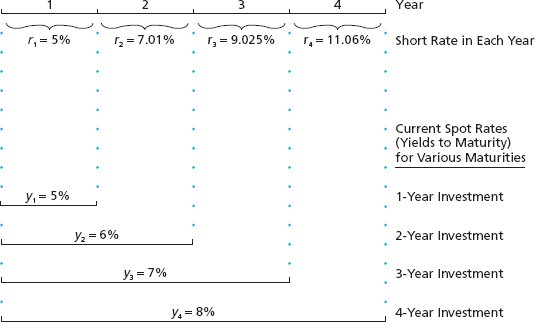
\includegraphics[width=6in]{pg486_3.jpg}


\subsection{General Short Rates}
\label{termStructure:general-short-rates}
We can generalize the previous results.
\begin{itemize}
\item {} 
Investing in an $n$ period zero-coupon bond should be the same
as investing in an $n-1$ zero and rolling into a one-period
zero at time $n-1$.

\end{itemize}
\begin{gather}
\begin{split}(1+y_n)^n & = (1+y_{n-1})^{n-1} \times (1+r_n)\end{split}\notag
\end{gather}\begin{gather}
\begin{split}\Rightarrow 1+r_n & = \frac{(1+y_n)^n}{(1+y_{n-1})^{n-1}}.\end{split}\notag
\end{gather}

\subsection{Forward Rates}
\label{termStructure:forward-rates}
In the development above, we assumed no uncertainty.
\begin{itemize}
\item {} 
All future rates were known at time zero.

\end{itemize}
\begin{itemize}
\item {} 
In reality, we don't have perfect knowledge of time $n$ short
rates at time zero.

\end{itemize}


\subsection{Forward Rates}
\label{termStructure:id7}
To distinguish between actual short rates that occur in the future, we
define the forward rate to be
\begin{gather}
\begin{split}\Rightarrow 1+f_n & = \frac{(1+y_n)^n}{(1+y_{n-1})^{n-1}}.\end{split}\notag
\end{gather}\begin{itemize}
\item {} 
The time $t=n$ forward rate is the break-even interest rate
that equates the returns of an n-period zero-coupon bond with an
$(n-1)$ -period zero rolled into a one-period zero.

\end{itemize}
\begin{itemize}
\item {} 
It may not be equal to the expected future short rate.

\end{itemize}


\subsection{Expectations Hypothesis}
\label{termStructure:expectations-hypothesis}
The \emph{Expectations Hypothesis} of the yield curve says that expected
short rates equal forward rates:
\begin{gather}
\begin{split}E[r_n] & = f_n\end{split}\notag
\end{gather}\begin{gather}
\begin{split}\Rightarrow (1+y_n)^n & = (1+y_{n-1})^{n-1}(1+E[r_n]).\end{split}\notag
\end{gather}\begin{itemize}
\item {} 
If the yield curve slopes upward, short rates are expected to rise:
$E[r_n] > E[r_{n-1}] > r_1 = y_1$.

\end{itemize}
\begin{itemize}
\item {} 
If the yield curve slopes downward, short rates are expected to
fall: $E[r_n] < E[r_{n-1}] < r_1 = y_1$.

\end{itemize}


\subsection{Liquidity Preference Theory}
\label{termStructure:liquidity-preference-theory}
According to the \emph{Liquidity Preference Theory} of the yield curve,
investors must be compensated for holding longer-term bonds.
\begin{itemize}
\item {} 
Longer-term bonds are subject to greater risk, and so investors
should demand a premium for holding them.

\end{itemize}
\begin{itemize}
\item {} 
In reality, a \emph{premium} means that investors will only buy them for
a lower price (which means greater yield).

\end{itemize}


\subsection{Liquidity Preference Theory}
\label{termStructure:id8}
The Liquidity Preference Theory can be expressed as forward rates
being equal to expected short rates plus a premium, $\phi$:
\begin{gather}
\begin{split}f_n & = E[r_n] + \phi\end{split}\notag
\end{gather}\begin{gather}
\begin{split}\Rightarrow (1+y_n)^n & = (1+y_{n-1})^{n-1}(1+E[r_n] + \phi).\end{split}\notag
\end{gather}\begin{itemize}
\item {} 
According to this theory, expected short rates \emph{can be} constant if
the yield curve is upward sloping.

\end{itemize}
\begin{itemize}
\item {} 
If the yield curve is downward sloping, expected short rates must be
falling. Why?

\end{itemize}


\subsection{Liquidity Preference Example}
\label{termStructure:liquidity-preference-example}
Suppose you buy a two-year bond and that
\begin{itemize}
\item {} 
Short rates for the next two years are constant at 8\%: $r_1 =
E[r_2] = 0.08$.

\end{itemize}
\begin{itemize}
\item {} 
The liquidity premium for year two is 1\%: $\phi = 0.01$.

\end{itemize}


\subsection{Liquidity Preference Example}
\label{termStructure:id9}
What is the yield to maturity of the two year bond?
\begin{gather}
\begin{split}(1+y_2)^2 & = (1+r_1)(1+f_2) \hspace{1.25in}\end{split}\notag
\end{gather}\begin{gather}
\begin{split}& = (1+r_1)(1+E[r_2]+\phi)\end{split}\notag
\end{gather}\begin{gather}
\begin{split}& = (1.08)(1.09) \hspace{0.8in}\end{split}\notag
\end{gather}\begin{gather}
\begin{split}\Rightarrow 1+y_2 & = \sqrt{1.08 \times 1.09} \hspace{1.4in}\end{split}\notag
\end{gather}\begin{gather}
\begin{split}& = 1.085. \hspace{1.2in}\end{split}\notag
\end{gather}\begin{itemize}
\item {} 
So the yield curve slopes up ($y_2 > y_1$) even though
expected short rates are constant.

\end{itemize}


\subsection{Expectations Hypothesis Example}
\label{termStructure:expectations-hypothesis-example}
However, if there is no liquidity premium
\begin{gather}
\begin{split}(1+y_2)^2 & = (1+r_1)(1+f_2) \hspace{0.95in}\end{split}\notag
\end{gather}\begin{gather}
\begin{split}& = (1+r_1)(1+E[r_2]) \hspace{0.02in}\end{split}\notag
\end{gather}\begin{gather}
\begin{split}& = (1.08)(1.08) \hspace{0.5in}\end{split}\notag
\end{gather}\begin{gather}
\begin{split}\Rightarrow 1+y_2 & = \sqrt{1.08 \times 1.08} \hspace{1.1in}\end{split}\notag
\end{gather}\begin{gather}
\begin{split}& = 1.08. \hspace{1in}\end{split}\notag
\end{gather}\begin{itemize}
\item {} 
Now the yield curve is flat.

\end{itemize}


\subsection{Implications of the Theories}
\label{termStructure:implications-of-the-theories}
The slope of the yield curve \emph{always} determines whether \emph{forward
rates} are rising or falling.
\begin{itemize}
\item {} 
$y_2 > y_1$ means $f_2 > f_1$ (by the definition of
forward rates!).

\end{itemize}
\begin{itemize}
\item {} 
If the Expectations Hypothesis holds, $E[r_2] = f_2$, so
$y_2 > y_1$ means $E[r_2] > r_1 = f_1 = y_1$.

\end{itemize}


\subsection{Implications of the Theories}
\label{termStructure:id10}\begin{itemize}
\item {} 
If the Liquidity Preference Theory holds, we have no guarantee that
$E[r_2] > r_1$ if $y_2 > y_1$.
\begin{itemize}
\item {} 
Short rates could be constant with a moderate liquidity premium.

\end{itemize}
\begin{itemize}
\item {} 
Short rates could be rising some, with a small liquidity premium.

\end{itemize}
\begin{itemize}
\item {} 
Short rates could be falling, with a large liquidity premium.

\end{itemize}
\begin{itemize}
\item {} 
What about if $y_2 < y_1$?

\end{itemize}

\end{itemize}


\subsection{Exp. Hypothesis vs. Liquidity Pref Theory}
\label{termStructure:exp-hypothesis-vs-liquidity-pref-theory}
$\qquad$

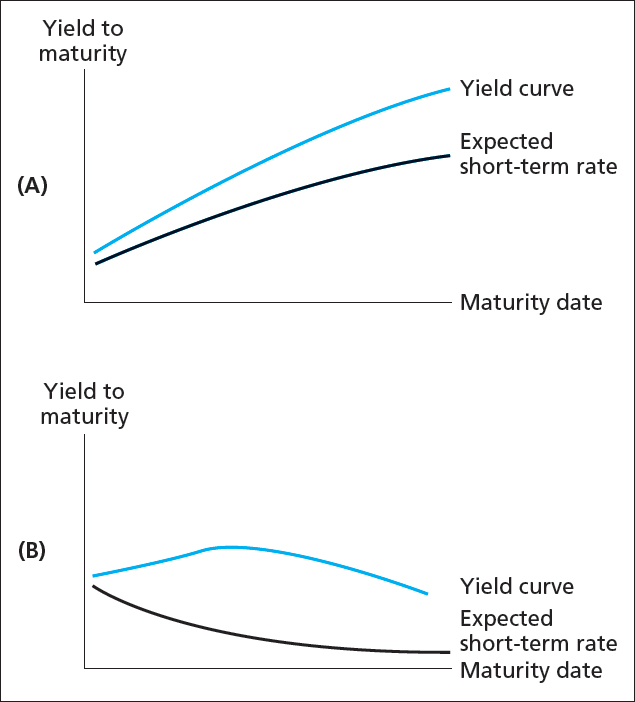
\includegraphics[width=6in]{bod34698_1014_lg.jpg}


\subsection{Historical Term Spread}
\label{termStructure:historical-term-spread}
$\qquad$

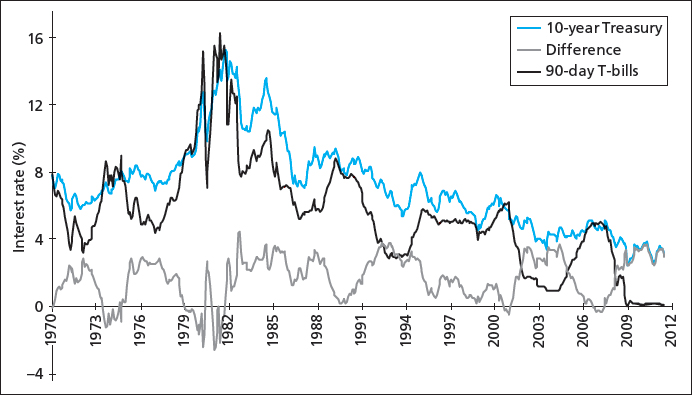
\includegraphics[width=6in]{bod34698_1015_lg.jpg}


\chapter{Options}
\label{options::doc}\label{options:options}

\section{Call Options}
\label{options:call-options}
A call option is a contract that allows the buyer the \emph{option} to
purchase an asset for a pre-specified price on or before a particular
date.  It has the following
ingredients:
\begin{itemize}
\item {} 
Underlying asset: The asset that may be bought or sold when the
option is exercised.

\end{itemize}
\begin{itemize}
\item {} 
Maturity (exercise) date: The date at which the contract expires.

\end{itemize}
\begin{itemize}
\item {} 
Strike price: The pre-specified price at which the underlying can be
purchased.

\end{itemize}


\section{Call Options}
\label{options:id1}
The buyer of the option is \emph{not obligated} to buy the underlying asset
at the strike price.
\begin{itemize}
\item {} 
The \emph{buyer} has the \emph{option} to buy.

\end{itemize}
\begin{itemize}
\item {} 
The \emph{seller} of the call option is \emph{obligated} to sell the
underlying if the buyer wants to exercise the option.

\end{itemize}
\begin{itemize}
\item {} 
If the price of the underlying asset is above the strike price on
the maturity date, the buyer will exercise. Why?

\end{itemize}
\begin{itemize}
\item {} 
If the price of the underlying asset is below the strike price on
the maturity date, the buyer will not exercise. Why?

\end{itemize}


\section{Call Options}
\label{options:id2}
The call option has no downside risk for the buyer.
\begin{itemize}
\item {} 
The buyer is better off if the underlying asset price rises.

\end{itemize}
\begin{itemize}
\item {} 
If the underlying asset price falls, the buyer doesn't lose
anything.

\end{itemize}


\section{Call Options}
\label{options:id3}
However, the seller of the option \emph{only} faces downside risk.
\begin{itemize}
\item {} 
The seller is worse off if the underlying asset price rises.

\end{itemize}
\begin{itemize}
\item {} 
If the underlying asset price falls, the seller doesn't gain
anything.

\end{itemize}

The seller must be compensated for taking the risk of having to sell
the underlying for a low price.
\begin{itemize}
\item {} 
The buyer pays a \emph{premium} to purchase the option contract.

\end{itemize}


\section{Call Option Example}
\label{options:call-option-example}
On March 8th 2013, stock for Chipotle Mexican Grill (CMG) sold for
\$321.84 and an option contract with a strike price of \$320.00 and
maturity date of March 15th 2013 cost \$5.30.
\begin{itemize}
\item {} 
If the price of Chipotle is less than \$320.00 on March 15th, the
option will not be exercised.

\end{itemize}
\begin{itemize}
\item {} 
If the price is \$325.00 on March 15th, the option holder (buyer)
will exercise the contract.

\end{itemize}
\begin{itemize}
\item {} 
The gain to the buyer will be \$5.00.

\end{itemize}


\section{Call Option Example}
\label{options:id4}\begin{itemize}
\item {} 
Remember that the contract cost \$5.30, so the buyer has a net loss
of \$0.30.

\end{itemize}
\begin{itemize}
\item {} 
If the price on March 15th is greater than \$325.30, the buyer will
have a net gain.

\end{itemize}


\section{Put Options}
\label{options:put-options}
A put option is a contract that allows the buyer the option to sell an
asset (the underlying) for a pre-specified price (the strike) on or
before a particular date (the maturity date).
\begin{itemize}
\item {} 
The buyer of the put benefits when the price of the underlying asset
falls below the strike.

\end{itemize}
\begin{itemize}
\item {} 
The buyer of the option can buy the asset at the market price and
sell it at the higher strike price (to the writer of the put
option).

\end{itemize}
\begin{itemize}
\item {} 
If the price of the asset rises above the strike, the buyer will not
exercise the option and has no downside loss.

\end{itemize}


\section{Put Options}
\label{options:id5}\begin{itemize}
\item {} 
The put is an \emph{option} (not an \emph{obligation}) for the buyer to sell
the asset at the strike price.

\end{itemize}
\begin{itemize}
\item {} 
The writer of the put is under \emph{obligation} to buy the asset
whenever the buyer chooses to exercise the option.

\end{itemize}


\section{Put Option Example}
\label{options:put-option-example}
Consider again Chipotle stock which sold for \$321.84 on March
8th 2013.
\begin{itemize}
\item {} 
A put option with a strike price of \$320.00 and a maturity date of
March 15th 2013 costs \$3.30.

\end{itemize}
\begin{itemize}
\item {} 
If the price of the stock is above \$320.00 on March 15th, the
option will not be exercised.

\end{itemize}


\section{Put Option Example}
\label{options:id6}\begin{itemize}
\item {} 
Suppose the price is below \$320.00 on March 15th: \$315.00.

\end{itemize}
\begin{itemize}
\item {} 
The buyer of the put will exercise the contract, buying the stock
for \$315.00 on the market and selling to the put writer for
\$320.00.

\end{itemize}
\begin{itemize}
\item {} 
The gross profit would be \$320.00 - \$315.00 = \$5.00.

\end{itemize}
\begin{itemize}
\item {} 
The net profit would be: \$5.00 - \$3.30.

\end{itemize}


\section{Moneyness}
\label{options:moneyness}
An option is
\begin{itemize}
\item {} 
\emph{In the money} when its strike price would produce profits for the
holder.

\end{itemize}
\begin{itemize}
\item {} 
\emph{Out of the money} when exercise would be unprofitable.

\end{itemize}
\begin{itemize}
\item {} 
\emph{At the money} when the strike price is equal to the asset price.

\end{itemize}

The moneyness can be determined at any time, as if the option were
exercised at that instant.


\section{American vs. European}
\label{options:american-vs-european}\begin{itemize}
\item {} 
An American option allows the buyer to exercise the contract on or
before the maturity date.

\end{itemize}
\begin{itemize}
\item {} 
A European option only allows exercise on the maturity date.

\end{itemize}
\begin{itemize}
\item {} 
Since an American option encompasses all of the possibilities of a
European option, it should always be more valuable and cost more.

\end{itemize}
\begin{itemize}
\item {} 
As the name denotes, virtually all options traded in the U.S. are of
the American flavor.

\end{itemize}


\section{Notation}
\label{options:notation}
We use the following notation:
\begin{gather}
\begin{split}T = \text{Maturity date}\end{split}\notag
\end{gather}\begin{gather}
\begin{split}S_t = \text{Underlying asset price at time } t\end{split}\notag
\end{gather}\begin{gather}
\begin{split}X = \text{Strike Price}\end{split}\notag
\end{gather}\begin{gather}
\begin{split}C_t = \text{Value of a call option at time } t\end{split}\notag
\end{gather}\begin{gather}
\begin{split}P_t = \text{Value of a put option at time } t\end{split}\notag
\end{gather}

\section{Call Option Payoff (Buyer)}
\label{options:call-option-payoff-buyer}
The payoff to a call option holder (buyer) at expiration is
\begin{gather}
\begin{split}C_T = \begin{cases} S_T - X, & \text{if  } S_T > X \\ 0, &
\text{if  } S_T \leq X. \end{cases}\end{split}\notag
\end{gather}\begin{itemize}
\item {} 
If the asset price is above the strike, the holder can buy the
underlying for $X$ and immediately sell it for $S_T$,
yielding a profit of $S_T-X$.

\end{itemize}
\begin{itemize}
\item {} 
If the asset price is below the strike, the option is worthless.

\end{itemize}


\section{Call Option Payoff (Buyer)}
\label{options:id7}
The payoffs above did not account for the cost of the option.
\begin{itemize}
\item {} 
If the option is purchased at time $t$ for a price of
$C_t$, the net payoff to the holder at expiration is

\end{itemize}
\begin{gather}
\begin{split}C_T = \begin{cases} S_T - X - C_t, & \text{if  } S_T > X \\ -C_t, &
\text{if  } S_T \leq X. \end{cases}\end{split}\notag
\end{gather}

\section{Call Option Payoff (Buyer}
\label{options:id8}
$\qquad$

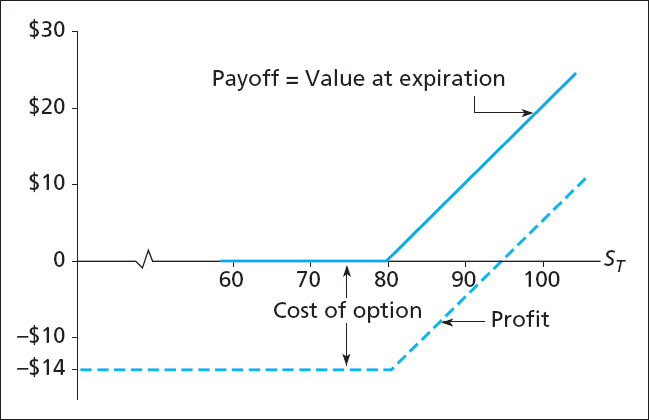
\includegraphics[width=6in]{bod34698_1502_lg.jpg}


\section{Call Option Payoff (Seller)}
\label{options:call-option-payoff-seller}
On the flip side, the gross payoff to the call option writer at
expiration is
\begin{gather}
\begin{split}C_T & = \begin{cases} X - S_T, & \text{if  } S_T > X
\\ 0, & \text{if  } S_T \leq X. \end{cases}\end{split}\notag
\end{gather}
The net payoff is
\begin{gather}
\begin{split}C_T & = \begin{cases} X - S_T + C_t, & \text{if  } S_T > X
\\ C_t, & \text{if  } S_T \leq X. \end{cases}\end{split}\notag
\end{gather}

\section{Call Option Payoff (Seller)}
\label{options:id9}
$\qquad$

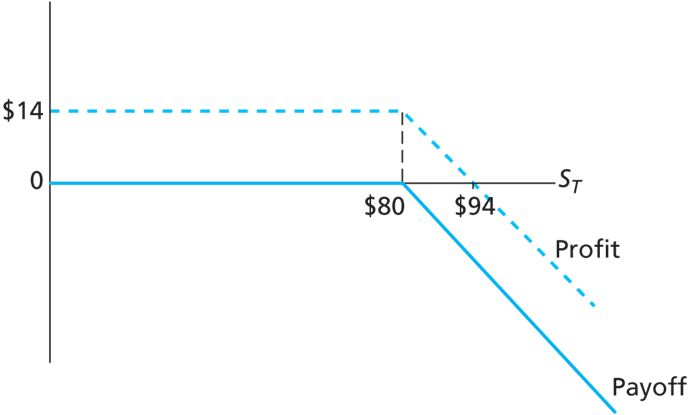
\includegraphics[width=6in]{bod34698_1503_lg.jpg}


\section{Put Option Payoff (Buyer)}
\label{options:put-option-payoff-buyer}
The gross payoff to put option holders at expiration is
\begin{gather}
\begin{split}P_T & = \begin{cases} 0, & \text{if  } S_T > X
\\ X - S_T, & \text{if  } S_T \leq X. \end{cases}\end{split}\notag
\end{gather}\begin{itemize}
\item {} 
If the underlying asset price is below the strike, the holder can
purchase it for $S_T$ and immediately resell for $X$,
yielding a profit of $X-S_T$.

\end{itemize}
\begin{itemize}
\item {} 
If the asset price is above the strike at expiration, the option is
worthless.

\end{itemize}


\section{Put Option Payoff (Buyer)}
\label{options:id10}
The \emph{net} payoff to put option holders is
\begin{gather}
\begin{split}P_T & = \begin{cases} -P_t, & \text{if  } S_T > X
\\ X - S_T - P_t, & \text{if  } S_T \leq X. \end{cases}\end{split}\notag
\end{gather}

\section{Put Option Payoff (Buyer)}
\label{options:id11}
$\qquad$

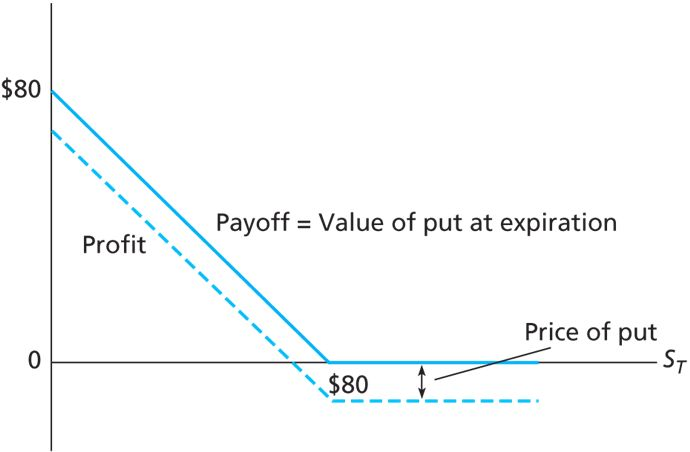
\includegraphics[width=6in]{bod34698_1504_lg.jpg}


\section{Speculation and Hedging}
\label{options:speculation-and-hedging}
Options can be used for both speculation and hedging.
\begin{itemize}
\item {} 
Suppose you have \$10,000 available for investment.

\end{itemize}
\begin{itemize}
\item {} 
A share of stock costs \$100.

\end{itemize}
\begin{itemize}
\item {} 
An option with a strike price of \$100 and six-month maturity costs
\$10.

\end{itemize}
\begin{itemize}
\item {} 
You can lend money (purchase the risk-free asset) at a rate of 3\%
for the next six months.

\end{itemize}


\section{Speculation and Hedging}
\label{options:id12}
Consider three strategies.
\begin{itemize}
\item {} 
Strategy A: Invest entirely in stock, buying 100 shares at the
current price of \$100.

\end{itemize}
\begin{itemize}
\item {} 
Strategy B: Invest entirely in at-the-money options, buying 10 call
contracts (each for 100 shares) selling for \$1000 a piece.

\end{itemize}
\begin{itemize}
\item {} 
Strategy C: Purchase 100 call options (1 contract) for \$1,000 and
invest the remaining \$9,000 in the risk-free asset, which will
yield a total of $\$9,000\times1.03 = \$9,270$ at the
end of the six months.

\end{itemize}


\section{Speculation and Hedging}
\label{options:id13}
The values of the three strategies are:

$\qquad$

{\hfill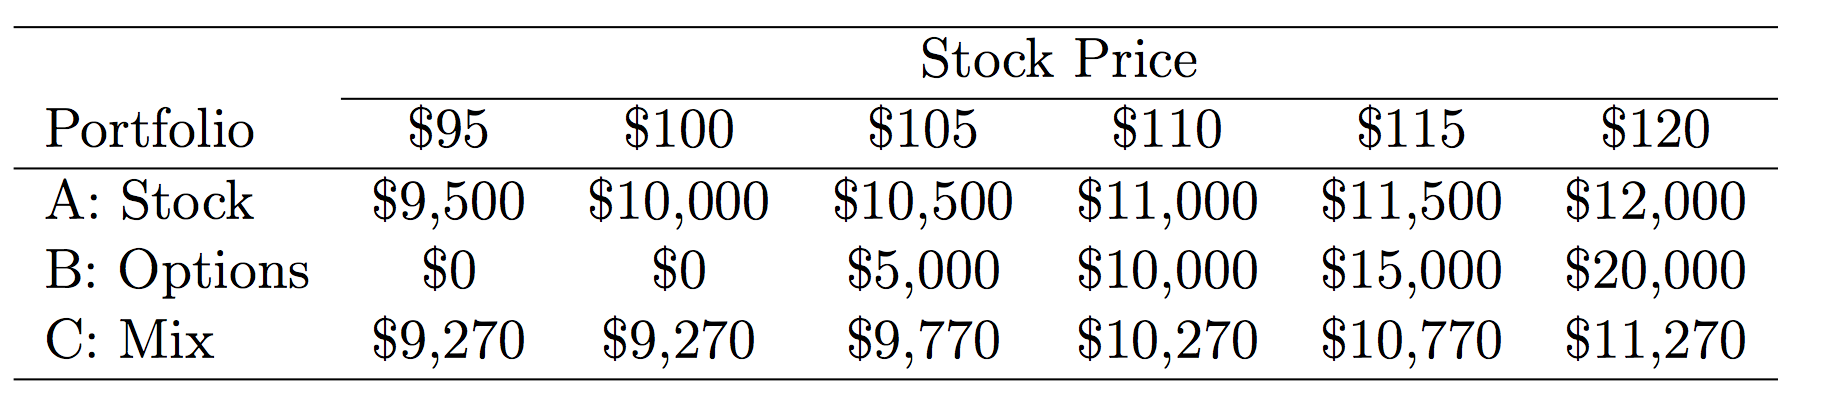
\includegraphics[width=8in]{table1.png}\hfill}


\section{Speculation and Hedging}
\label{options:id14}
The returns to the three strategies are:

$\qquad$

{\hfill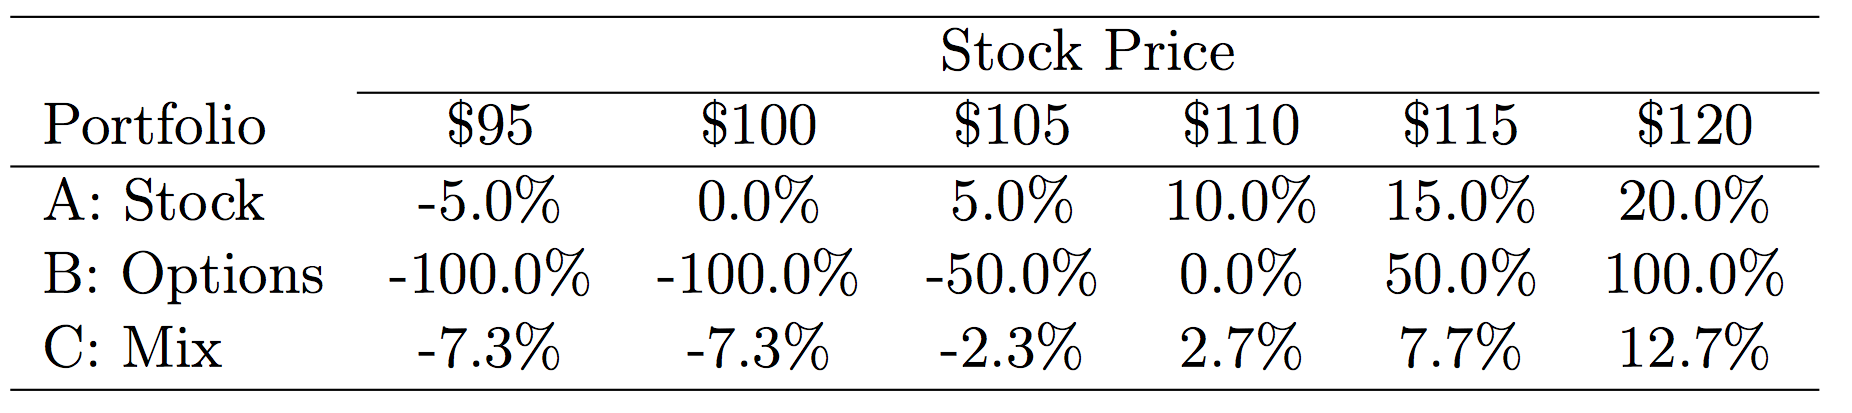
\includegraphics[width=8in]{table2.png}\hfill}


\section{Speculation and Hedging}
\label{options:id15}
From these tables we see two features of options.
\begin{itemize}
\item {} 
Options offer leverage.
\begin{itemize}
\item {} 
For the all-option portfolio, the return plummets to -100\% when
the stock price is below the strike.

\end{itemize}
\begin{itemize}
\item {} 
The return rockets to numbers that are much greater than simply
holding the stock when the stock price increases above the
strike.

\end{itemize}

\end{itemize}


\section{Speculation and Hedging}
\label{options:id16}\begin{itemize}
\item {} 
Options offer insurance.
\begin{itemize}
\item {} 
The mixed portfolio has limited downside loss: the investor can't
lose more than -7.3\%.

\end{itemize}
\begin{itemize}
\item {} 
It also has limited upside gains: if the stock price is above the
strike, its returns are always below the portfolio comprised of
only stock.

\end{itemize}

\end{itemize}


\section{Speculation and Hedging}
\label{options:id17}
$\qquad$

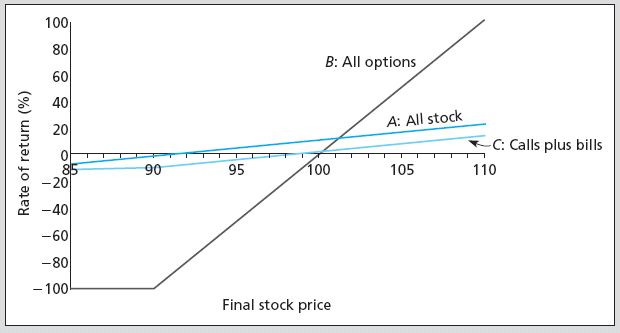
\includegraphics[width=6in]{bod34698_1505_lg.jpg}


\section{Protective Put}
\label{options:protective-put}
A protective put strategy consists of simultaneously purchasing a
share of stock and a put option on that stock.
\begin{itemize}
\item {} 
This limits the potential downside loss of the stock while leaving
the potential gains intact.

\end{itemize}

$\qquad$

{\hfill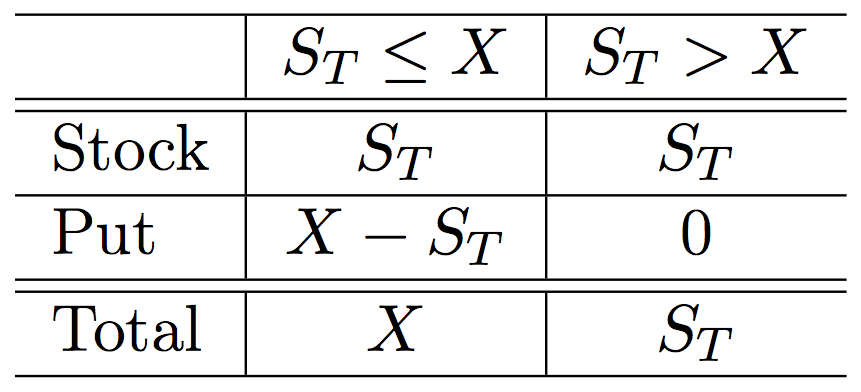
\includegraphics[width=4in]{table3.png}\hfill}


\section{Protective Put}
\label{options:id18}
The put acts as insurance against loss.
\begin{itemize}
\item {} 
Comparing the net payoff of the protective put with the strategy of
holding stock alone shows that the former comes at a cost.

\end{itemize}
\begin{itemize}
\item {} 
This is the insurance premium.

\end{itemize}


\section{Protective Put}
\label{options:id19}
$\qquad$

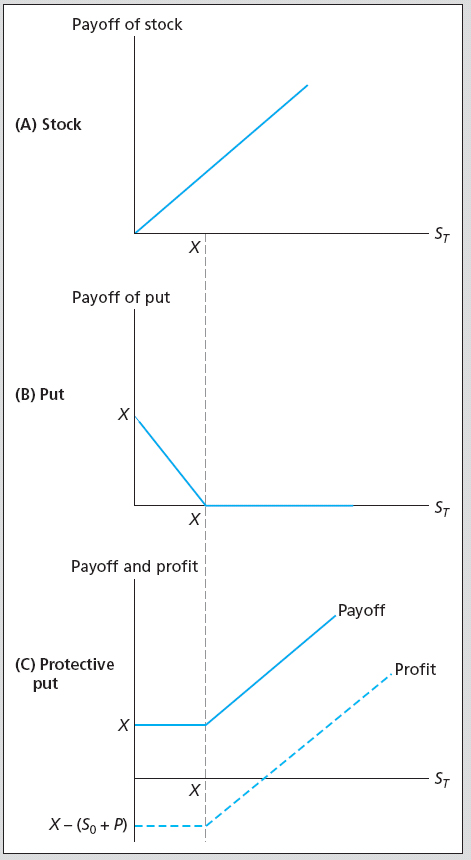
\includegraphics[width=4in]{bod34698_1506_lg.jpg}


\section{Protective Put}
\label{options:id20}
$\qquad$

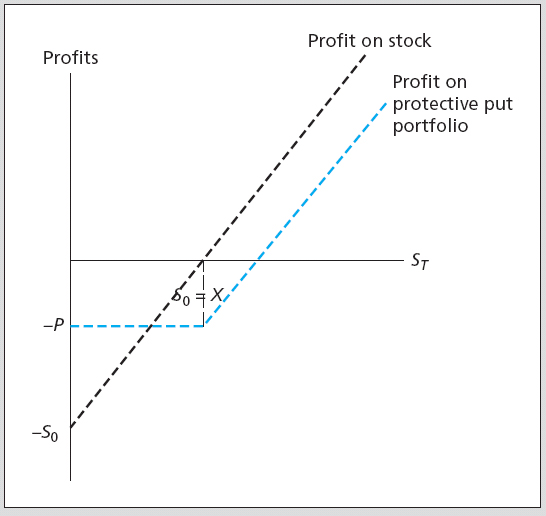
\includegraphics[width=5in]{bod34698_1507_lg.jpg}


\section{Covered Call}
\label{options:covered-call}
A covered call strategy consists of simultaneously purchasing a share
of stock and writing a call option on that stock.
\begin{itemize}
\item {} 
It doesn't eliminate downside loss (like the protective put).

\end{itemize}
\begin{itemize}
\item {} 
It covers the obligation to deliver the stock for less than its
market value if the stock price is above the strike.

\end{itemize}
\begin{itemize}
\item {} 
The call writer is charging a premium (the call price) in order to
forsake the upside gain of holding the stock.

\end{itemize}

{\hfill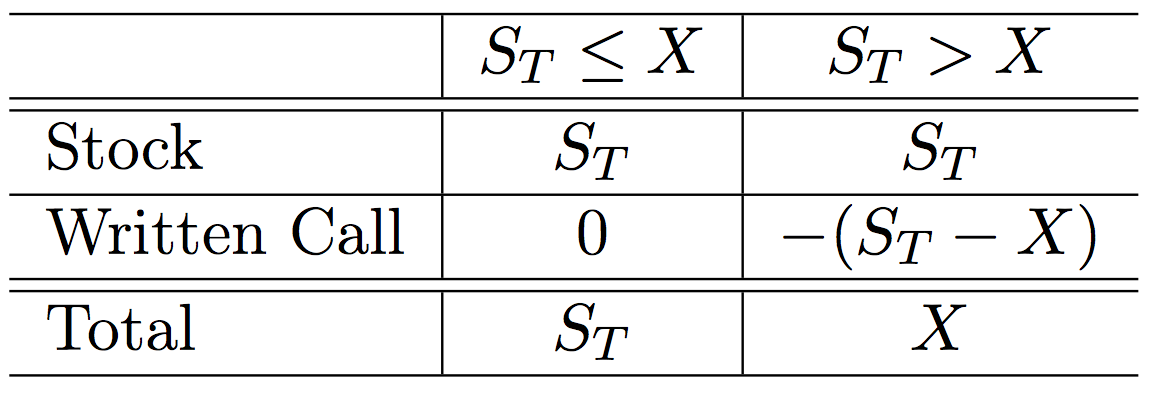
\includegraphics[width=5in]{table4.png}\hfill}


\section{Covered Call}
\label{options:id21}
$\qquad$

\includegraphics[width=4in]{bod34698_1508_lg.jpg}


\section{Straddle}
\label{options:straddle}
A straddle consists of purchasing call and put options for the same
asset and strike price.
\begin{itemize}
\item {} 
It is a bet on volatility.

\end{itemize}
\begin{itemize}
\item {} 
The straddle holder will earn (gross) positive returns if the stock
price moves up or down, but nothing if it remains at the strike.

\end{itemize}

$\qquad$

{\hfill\includegraphics[width=4in]{table5.png}\hfill}


\section{Straddle}
\label{options:id22}
So why doesn't everyone hold straddles?
\begin{itemize}
\item {} 
Because the investor must pay for both contracts.

\end{itemize}
\begin{itemize}
\item {} 
The investor doesn't earn a \emph{net} return unless the stock price
moves enough to compensate for the initial outlay.

\end{itemize}


\section{Straddle}
\label{options:id23}
$\qquad$

\includegraphics[width=4in]{bod34698_1509_lg.jpg}


\section{Spread}
\label{options:spread}
A spread is a combination of two or more options (both calls or both
puts) on the same stock with different strikes.
\begin{itemize}
\item {} 
Some of the options are purchased while others are sold.

\end{itemize}
\begin{itemize}
\item {} 
A money spread is the simultaneous purchase and sale of options with
different strikes.

\end{itemize}
\begin{itemize}
\item {} 
A time spread is the simultaneous purchase and sale of options with
different maturities.

\end{itemize}


\section{Bullish Spread}
\label{options:bullish-spread}
A bullish spread:

$\qquad$

{\hfill\includegraphics[width=7in]{table6.png}\hfill}


\section{Bullish Spread}
\label{options:id24}
$\qquad$

\includegraphics[width=4in]{bod34698_1510_lg.jpg}


\section{Collar}
\label{options:collar}
An example of a collar is the purchase of a protective put for one
strike price and the sale of a call option, on the same stock, for a
higher strike.
\begin{itemize}
\item {} 
This strategy eliminates downside losses below the strike of the put
and also upside gains beyond the strike of the call.

\end{itemize}
\begin{itemize}
\item {} 
In this case, the investor constrains gains and losses within a
region close to the current price of the stock.

\end{itemize}


\section{Protective Put Alternative}
\label{options:protective-put-alternative}
A protective put eliminates the downside loss of holding stock. We
could achieve this with an alternative strategy.
\begin{itemize}
\item {} 
Purchase a call option with strike price $X$.

\end{itemize}
\begin{itemize}
\item {} 
Purchase a T-bill (lend at the risk-free rate) with a face value
equal to the call strike price, $X$, and the same maturity
date as the call.

\end{itemize}

$\qquad$

{\hfill\includegraphics[width=4in]{table7.png}\hfill}


\section{Put Call Parity}
\label{options:put-call-parity}
The payoffs in the previous table are identical to those for the
protective put.
\begin{itemize}
\item {} 
Hence, the cost of the protective put strategy should be equal to
the cost of the call plus bonds strategy (why?!!!).

\end{itemize}
\begin{itemize}
\item {} 
This fact is known as the \emph{Put-Call Parity Relationship}.

\end{itemize}
\begin{itemize}
\item {} 
Mathematically, it can be expressed as:

\end{itemize}
\begin{gather}
\begin{split}C_0 + \frac{X}{1+r_f} & = S_0 + P_0.\end{split}\notag
\end{gather}\begin{itemize}
\item {} 
This relationship is very useful because it allows us to compute the
value of a call option if we know the price of the corresponding
put, and vice versa.

\end{itemize}


\section{Put Call Parity Example}
\label{options:put-call-parity-example}
Assume
\begin{itemize}
\item {} 
An asset currently sells for \$110.

\end{itemize}
\begin{itemize}
\item {} 
A call option with strike $X = \$105$ and 1-year maturity
sells for \$17.

\end{itemize}
\begin{itemize}
\item {} 
A put option with strike $X = \$105$ and 1-year maturity
sells for \$5.

\end{itemize}
\begin{itemize}
\item {} 
The risk-free interest rate is 5\% per year.

\end{itemize}
\begin{itemize}
\item {} 
Does the parity relationship hold?

\end{itemize}


\section{Put Call Parity Example}
\label{options:id25}\begin{gather}
\begin{split}C_0 + \frac{X}{1+r_f} & \stackrel{?}{=} S_0 + P_0.\end{split}\notag
\end{gather}\begin{gather}
\begin{split}\$117 = \$17 + \frac{\$105}{1.05} & \neq \$110 + \$5 = \$115.\end{split}\notag
\end{gather}\begin{itemize}
\item {} 
The relationship doesn't hold.

\end{itemize}
\begin{itemize}
\item {} 
How might an investor take advantage of the situation?

\end{itemize}


\section{Put Call Parity Example}
\label{options:id26}
$\qquad$

{\hfill\includegraphics[width=7in]{table8.png}\hfill}



\renewcommand{\indexname}{Index}
\printindex
\end{document}
